\chapter{Validación Experimental} % Main chapter title

\label{Chapter6}


En este capítulo se lleva a cabo la validación experimental, demostrando que controlando la diversidad en el espacio de las variables es una forma para mejorar los resultados obtenidos en comparación al estado-del-arte de MOEAs. 
%
Por lo tanto, únicamente son analizados los resultados más significativos y el resto puede ser consultado en el apéndice.
%
En la primera parte de este estudio experimental se analiza el comportamiento del VSD-MOEA junto con los algoritmos que pertenecen al estado-del-arte, adicionalmente se analiza la escalabilidad en el espacio de las variables de este conjunto.
%
En ese orden, se demuestra la estabilidad del VSD-MOEA con distintas configuraciones en el parámetro que indica el grado de diversidad inicial.
%
En la segunda parte, son analizados los resutados obtenidos por las propuestas basadas en descomposición, donde se discute el MOEA/D-EVSD que promueve la diversidad de forma implícita, y aparte se discuten los algoritmos MOEA/D-SEBV y VSD-MOEA/D que fomentan la diversidad explícitamente.
%
%
Finalmente, se examina el operador de cruce NRD-SBX comparado al clásico operador SBX.

%

\section{Esquema de validación experimental}

En esta sección se especifican los análisis estadísticos y configuraciones, que junto a los indicadores y superficies de cubrimiento (definidos en el capítulo \ref{Chapter1}) son utilizados para llevar a cabo la validación experimental.
%
Como parte de este proceso se utilizaron los algoritmos implementados en el jMetalcpp por \cite{Joel:jMetal}.
%
Además se seleccionaron los problemas de prueba WFG (\cite{Joel:WFG}), DTLZ (\cite{Joel:DTLZ_2}), UF (\cite{Joel:CEC2009}).
%

Dado que todos los optimizadores son estocásticos, cada ejecución se repitió $35$ veces con diferentes semillas en el generador de números aleatorios.
%
Los siguientes aspectos fueron comunes para todos los algoritmos: el criterio de parada se fijó a $250,000$ generaciones, el tamaño de población a $100$, el operador de cruce SBX o NRD-SBX se configuró con un índice de distribución igual a $20$ y la probabilidad de su uso fue de $0.9$, se utilizó la mutación polinomial con un índice de distribución igual a $50$ y su probabilidad se fijó a $1/n$, donde $n$ es el número de variables.
%
%
Además, para dos y tres objetivos los problemas WFG fueron configurados con $24$ parámetros, siendo $20$ de ellos parámetros de distancia, y $4$ de ellos parámetros de posición.
%
En los problemas de prueba DTLZ, el número de variables es asignado a $n = M + r -1$, donde $r=\{5,10,20\}$ para el DTLZ1, DTLZ2 - DTLZ6 y DTLZ7 respectivamente, como es sugerido por los autores \cite{Joel:DTLZ_2}.
%
Los problemas de prueba UF están compuestos de diez instancias, donde las primeras siete corresponden a dos objetivos y el resto a tres objetivos, además para todos los problemas el número de variables es asignado a $n=30$.
%
La parametrización específica de cada algoritmo es mostrado en la tabla \ref{tab:Parametrization}.
%

\begin{table}[h]
\centering
\caption{Parametrización}
\label{tab:Parametrization}
\begin{tabular}{l|l}
\hline
\textbf{Algoritmo} & \textbf{Configuración} \\ \hline
GDE3 & $CR = 0.9$ y $F = 0.5$ \\ \hline
SMS-EMOA& desplazamiento = 250 \\ \hline
MOMBI-II & $\epsilon = 1e-3$, $\alpha = 0.5$, tamaño del registro = $5$ generaciones \\ \hline
MOEA/D & \begin{tabular}[c]{@{}l@{}} tamaño de la vecindad $T = 20$, \\ max actualizaciones por sub-problema ($\eta_r$) = 2 y $\delta = 0.9$\end{tabular} \\ \hline
MOEA/D-EVSD & \begin{tabular}[c]{@{}l@{}} en la primer fase se utiliza un 80\% del total de generaciones, \\ en la segunda fase utiliza 20\% del total de generaciones,\\ $\alpha$ = 20 individuos, $T_{r,1}$ = 2, $T_{r,2}$ = 25 \end{tabular} \\ \hline
VSD-MOEA-SEBV  & $D_I=\sqrt{n}*0.2$, $CR = 0.9$, $F=0.5$, $T=10$ \\ \hline
VSD-MOEA/D & $D_I=\sqrt{n}*0.2$, $F = 0.5$, $T=10$ \\ \hline
VSD-MOEA & $D_I=\sqrt{n}*0.2$ \\ \hline
\end{tabular}
\end{table}

%
En orden para comparar estadísticamente los resultados de cada métrica (hipervolumen, IGD+, $\Delta_p$), y teniendo en cuenta el comportamiento estocástico de los optimizadores, se realizaron un conjunto de pruebas estadísticas como se muestra en la figura \ref{fig:Tests} (\cite{Joel:StatisticalTest}). 
%

Concretamente, en primer lugar se utiliza la prueba Shapiro-Wilk para comprobar si los resultados se ajustan a una distribución Gaussiana. 
%
En los casos en que sí se ajusten, se utiliza la prueba de Levene para comprobar la homogeneidad de las varianzas, procediendo con la prueba de ANOVA en caso positivo o con el de Welch en caso negativo.
%
Por otro lado, para los casos que no se ajusten a distribuciones Guassianas, se utiliza la prueba de Kruskal-Wallis.
%
En todos los casos es fijado el nivel de confianza al 95\%.
%
Se considera que un algoritmo $X$ es superior a un algoritmo $Y$, si el procedimiento anterior reporta diferencias significativas, además si la media y mediana del indicador obtenido por el método $X$ son superiores a las obtenidas por el método $Y$.
\begin{figure}[H]
\centering
\scriptsize
%\includegraphics[width=6cm, height=6cm]
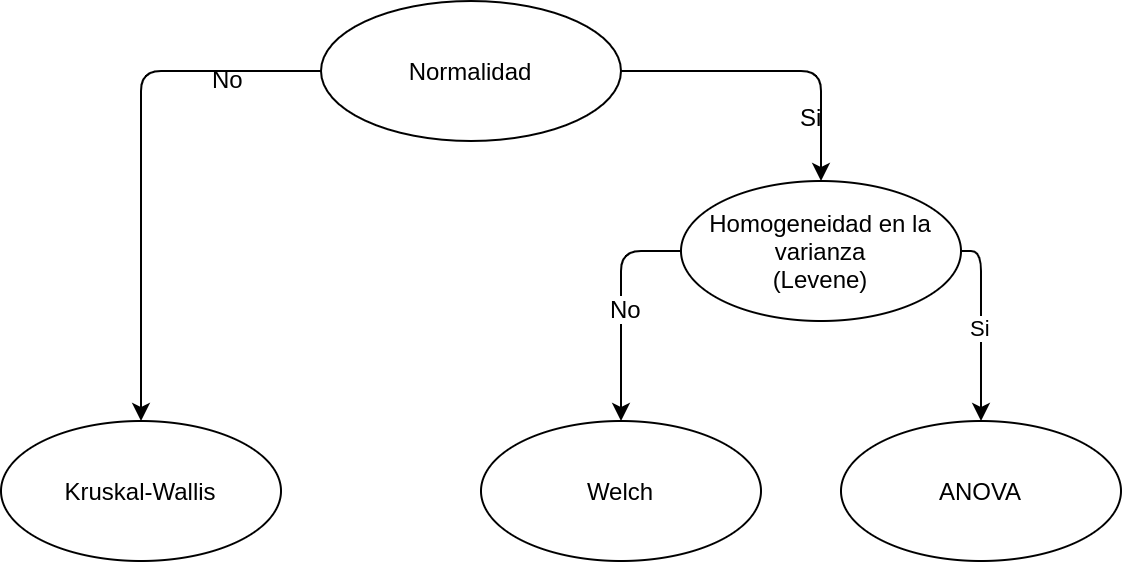
\includegraphics[scale=0.2]
{Figures_Chapter6/Tests.png}
\caption{Pruebas estadísticas para determinar la superioridad de un algoritmo.}
\label{fig:Tests}
\end{figure}


Los resultados estadísticos de cada métrica se describen en base a las estadísticas generales, pruebas estadísticas y pruebas efectivas.
%
En las estadísticas generales en relación a un determinado indicador es presentado el mínimo, máximo y la media, adicionalmente se indica la columna \textit{Diff} que representa el grado de diferencia con el mejor resultado de cada algoritmo, por lo tanto el mejor algoritmo en cada instancia tiene un valor en \textit{Diff} de cero.
%
Las pruebas estadísticas son realizadas por medio de comparaciones entre cada par de algorimos, así para cada instancia y cada algoritmo, la columna $\uparrow$ reporta el número de comparaciones donde las pruebas estadísticas confirman la superioridad de cada algoritmo, mientras que la columna $\downarrow$ reporta el número de casos en que ese algoritmo es inferior.
%
Similarmente, las pruebas efectivas cualifican la superioridad de cada algoritmo con el resto a través de comparaciones por pares.
%
Así, si un algoritmo \textbf{A} es comparado con un algoritmo \textbf{B}, si \textbf{A} gana, se acumula la diferencia con \textbf{B} en la columna de ganancia $\uparrow$ que corresponde al algoritmo \textbf{A}, de igual forma se acumula esta diferencia en la columna de perdida $\downarrow$ en el algoritmo \textbf{B}.
%
La columna de \textit{Puntaje} indica la diferencia total entre las comparaciones ganadas y las perdidas, por lo tanto un puntaje elevado indica la superioridad del algoritmo.
%

Para realizar el cálculo del indicador que corresponde al hipervolumen, en cada problema se escoge como vector de referencia al vector nadir más un incremento, donde el incremento es pequeño para problemas sencillos y la unidad para problemas complejos.
%
Así, los puntos de referencia implementados en el indicador del hipervolumen se muestran en la tabla \ref{tab:ReferencePoints} como son utilizados en \cite{berengueroptimizacion}.

\begin{table}[H]
\centering
\caption{Puntos de referencia para el indicador del hipervolumen}
\label{tab:ReferencePoints}
\begin{tabular}{cc}
\hline
\textbf{Instancias} & \textbf{Punto de referencia} \\ \hline
WFG1-WFG9 & $[2.1, ...,2m+0.1]$ \\
DTLZ 1, 2, 4 & $[1.1, ..., 1.1]$ \\
DTLZ 3, 5, 6 & $[3, ..., 3]$ \\
DTLZ7 & $[1.1, ..., 1.1, 2m]$ \\
UF 1-10 & $[2, ..., 2]$ \\ \hline
\end{tabular}
\end{table}



\section{Algoritmo basado en dominancia VSD-MOEA}

En esta sección se lleva a cabo la validación experimental de la propuesta de diversidad basada en dominancia, donde es comparado con el estado-del-arte de los MOEAs.
% 
Para realizar el análisis de los resultados se utiliza el indicador del hipervolumen, distancia generacional invertida (IGD+) y la distancia de hausdorff ($\Delta_p$), de cada indicador se reporta la tabla de estadísticas, pruebas estadísticas y pruebas efectivas, principalmente se discuten los resultados que corresponden al indicador del hipervolumen, el resto del material se puede consultar en el apéndice \ref{AppendixA}.

Inicialmente, los resultados estadísticos que corresponden a dos objetivos, son presentados en la tabla \ref{tab:StatisticsHV_2obj_exp}, se puede apreciar que el algoritmo GDE3 proporciona los mejores resultados en la mayorías de las instancias, a pesar de eso la suma total de todas las diferencias entre este algoritmo y el mejor es menor que la que posee el VSD-MOEA/D, esto indica que aunque el GDE3 es superior en la mayoría de problemas, su rendimiento es significativamente malo en otras instancias de prueba.
%
Por otra parte, nuestra propuesta es suficientemente estable ya que ofrece soluciones muy cercanas a los mejores valores encontrados, y en consecuencia es indicada una menor diferencia.
%

Es importante mencionar que el conjunto de prueba DTLZ tiene los siguientes inconvenientes (\cite{zhang2008multiobjective}).
%
El óptimo global está ubicado en el centro o en los límites del espacio factible, todos los problemas son separables y el óptimo global tiene los mismos valores en todas las variables del espacio factible.
%
Particularmente, el DTLZ5 y DTLZ6 son problemas sencillos para el GDE3, ya que el óptimo global está ubicado en el límite inferor, por lo tanto al utilizar una estrategía para corregir a los individuos que violan los límites del espacio factible como es el \textit{método de proyección} (\cite{kreischerevaluation}), existirá una tendencia injusta hacia las regiones óptimas.
%
En la tabla \ref{tab:StatisticsHV_3obj_exp} se puede observar que conforme aumenta el número de objetivos empeora el desempeño del GDE3, por lo tanto para tres objetivos su diferencia con los mejores resultados son elevados, excepto para el DTLZ5 y DTLZ6 donde el conjunto óptimo es ubicado en la frontera del espacio factible.
%
El resto de algoritmos implementan el operador genético DNR-SBX, por lo tanto poseen un comportamiento diferente\footnote{Existen problemas numéricos con la implementación del operador SBX para ubicar individuos exactamente en la frontera del espacio factible.}.
%0
A pesar de eso, se puede observar que el VSD-MOEA ofrece soluciones suficientemente estables tanto en dos objetivos como en tres objetivos, inclusive al aumentar el número de objetivos\footnote{En el apéndice \ref{AppendixA} se presentan los resultados considerando diez objetivos.} proporciona mejores resultados que el resto de algoritmos basados en dominancia.
%
Principalmente, el VSD-MOEA resuelve mejor a los problemas de prueba más complejos, entre ellos los que poseen alta dependencia, multimodales y deceptivos.
%
Además, sus respectivos valores que corresponden al mínimo y máximo son superiores que los algoritmos del estado-del-arte.
%

En las tablas \ref{tab:Effective_Test_2obj_exp}, \ref{tab:Effective_Test_3obj_exp} se muestran los resultados que corresponden a las pruebas efectivas en dos y tre objetivos respectivamente.
%
Se puede observar que nuestra propuesta únicamente posee un puntaje negativo en las instancias DTLZ6 y WFG6 con dos objetivos, esto ocurre ya que estas instancias pueden ser fácilmente resueltas en esquemas a largo plazo y por lo tanto la calidad de los resultados se ve reflejado en base a la diversidad del espacio objetivo.
%
Además nuestra propuesta posee el mejor puntaje total, tanto en dos como en tres objetivos, ofreciendo soluciones de mayor calidad y por ende una mayor convergencia al frente de Pareto.

Particularmente, el MOEA/D y el MOMBI-II logran mejores resultados conforme aumenta el número de objetivos, principalmente porque su diseño es en base a los vectores de pesos que a diferencia del concepto de dominancia no decrementa la presión de selección.
%
Así, el MOMBI-II con dos objetivos proporciona los peores resultados en comparación a los demás algoritmos, pero con tres objetivos se observa que su puntaje mejora significativamente siendo el segundo mejor.

%
% Please add the following required packages to your document preamble:
% \usepackage{graphicx}
\begin{table}[H]
%\centering
\caption{Estadísticas del hipervolumen considerando dos objetivos}
\label{tab:StatisticsHV_2obj_exp}
\resizebox{\textwidth}{!}{%
 \begin{threeparttable}
\begin{tabular}{c|c|c|c|c|c|c|c|c|c|c|c|c|c|c|c|c|c|c|c|c|}
\cline{2-21}
                              & \multicolumn{4}{c|}{GDE3}                       & \multicolumn{4}{c|}{MOMBI-II}                   & \multicolumn{4}{c|}{NSGAII}            & \multicolumn{4}{c|}{MOEA/D}            & \multicolumn{4}{c|}{VSD-MOEA}                   \\ \cline{2-21} 
                              & Min   & Max   & Mean           & Diff           & Min   & Max   & Mean           & Diff           & Min   & Max   & Mean  & Diff           & Min   & Max   & Mean  & Diff           & Min   & Max   & Mean           & Diff           \\ \hline
\multicolumn{1}{|c|}{DTLZ1}   & 1.084 & 1.084 & \textbf{1.084} & 0.000          & 1.078 & 1.078 & 1.078          & 0.006          & 1.083 & 1.083 & 1.083 & 0.000          & 1.078 & 1.084 & 1.081 & 0.003          & 1.084 & 1.084 & \textbf{1.084} & 0.000          \\ \hline
\multicolumn{1}{|c|}{DTLZ2}   & 0.421 & 0.421 & \textbf{0.421} & 0.000          & 0.418 & 0.418 & 0.418          & 0.003          & 0.419 & 0.420 & 0.419 & 0.001          & 0.420 & 0.420 & 0.420 & 0.001          & 0.420 & 0.420 & 0.420          & 0.000          \\ \hline
\multicolumn{1}{|c|}{DTLZ3}   & 8.211 & 8.211 & \textbf{8.211} & 0.000          & 8.170 & 8.170 & 8.170          & 0.041          & 8.209 & 8.210 & 8.209 & 0.001          & 8.169 & 8.210 & 8.200 & 0.011          & 8.210 & 8.210 & 8.210          & 0.000          \\ \hline
\multicolumn{1}{|c|}{DTLZ4}   & 0.421 & 0.421 & \textbf{0.421} & 0.000          & 0.110 & 0.418 & 0.383          & 0.038          & 0.110 & 0.420 & 0.313 & 0.107          & 0.110 & 0.418 & 0.365 & 0.055          & 0.420 & 0.420 & 0.420          & 0.000          \\ \hline
\multicolumn{1}{|c|}{DTLZ5}   & 8.211 & 8.211 & \textbf{8.211} & 0.000          & 8.170 & 8.170 & 8.170          & 0.041          & 8.209 & 8.210 & 8.209 & 0.001          & 8.210 & 8.210 & 8.210 & 0.001          & 8.210 & 8.210 & \textbf{8.210} & 0.000          \\ \hline
\multicolumn{1}{|c|}{DTLZ6}   & 8.211 & 8.211 & \textbf{8.211} & 0.000          & 7.989 & 8.170 & 8.073          & 0.138          & 8.062 & 8.209 & 8.128 & 0.083          & 8.027 & 8.210 & 8.095 & 0.116          & 7.989 & 8.210 & 8.123          & 0.088          \\ \hline
\multicolumn{1}{|c|}{DTLZ7}   & 0.894 & 0.894 & \textbf{0.894} & 0.000          & 0.417 & 0.417 & 0.417          & 0.478          & 0.420 & 0.420 & 0.420 & 0.474          & 0.420 & 0.420 & 0.420 & 0.474          & 0.893 & 0.893 & 0.893          & 0.001          \\ \hline
\multicolumn{1}{|c|}{UF1}     & 3.657 & 3.659 & 3.658          & 0.002          & 3.327 & 3.517 & 3.490          & 0.171          & 3.650 & 3.652 & 3.651 & 0.010          & 3.428 & 3.660 & 3.588 & 0.072          & 3.655 & 3.662 & \textbf{3.661} & 0.000          \\ \hline
\multicolumn{1}{|c|}{UF2}     & 3.651 & 3.654 & 3.653          & 0.005          & 3.406 & 3.628 & 3.594          & 0.064          & 3.643 & 3.647 & 3.645 & 0.013          & 3.428 & 3.649 & 3.533 & 0.124          & 3.655 & 3.660 & \textbf{3.658} & 0.000          \\ \hline
\multicolumn{1}{|c|}{UF3}     & 3.371 & 3.660 & \textbf{3.642} & 0.000          & 3.328 & 3.595 & 3.499          & 0.143          & 3.524 & 3.639 & 3.602 & 0.041          & 2.850 & 3.642 & 3.451 & 0.191          & 3.549 & 3.620 & 3.593          & 0.049          \\ \hline
\multicolumn{1}{|c|}{UF4}     & 3.219 & 3.237 & 3.224          & 0.036          & 3.194 & 3.205 & 3.197          & 0.062          & 3.198 & 3.207 & 3.200 & 0.060          & 3.210 & 3.243 & 3.228 & 0.032          & 3.235 & 3.280 & \textbf{3.260} & 0.000          \\ \hline
\multicolumn{1}{|c|}{UF5}     & 2.532 & 3.000 & \textbf{2.964} & 0.000          & 2.047 & 2.746 & 2.522          & 0.442          & 1.861 & 2.897 & 2.602 & 0.362          & 1.800 & 2.550 & 2.185 & 0.778          & 2.591 & 3.267 & 2.951          & 0.013          \\ \hline
\multicolumn{1}{|c|}{UF6}     & 2.000 & 3.325 & \textbf{3.098} & 0.000          & 2.013 & 2.893 & 2.638          & 0.460          & 2.007 & 2.896 & 2.518 & 0.580          & 0.726 & 2.884 & 2.070 & 1.028          & 2.893 & 3.306 & 3.058          & 0.040          \\ \hline
\multicolumn{1}{|c|}{UF7}     & 3.490 & 3.492 & \textbf{3.491} & 0.000          & 2.474 & 3.470 & 2.592          & 0.899          & 2.168 & 3.485 & 3.190 & 0.301          & 2.015 & 3.493 & 2.743 & 0.748          & 3.473 & 3.493 & 3.489          & 0.002          \\ \hline
\multicolumn{1}{|c|}{WFG1}    & 4.263 & 5.256 & 4.848          & 0.408          & 4.623 & 5.666 & \textbf{5.256} & 0.000          & 4.716 & 5.250 & 5.156 & 0.100          & 4.480 & 5.243 & 5.037 & 0.219          & 4.717 & 5.250 & 5.205          & 0.051          \\ \hline
\multicolumn{1}{|c|}{WFG2}    & 5.072 & 5.072 & \textbf{5.072} & 0.000          & 4.925 & 4.942 & 4.927          & 0.145          & 4.948 & 5.068 & 4.953 & 0.119          & 4.943 & 4.943 & 4.943 & 0.128          & 5.069 & 5.069 & 5.069          & 0.003          \\ \hline
\multicolumn{1}{|c|}{WFG3}    & 4.513 & 4.530 & 4.522          & 0.043          & 4.561 & 4.563 & 4.562          & 0.003          & 4.533 & 4.543 & 4.539 & 0.026          & 4.562 & 4.563 & 4.563 & 0.002          & 4.565 & 4.565 & \textbf{4.565} & 0.000          \\ \hline
\multicolumn{1}{|c|}{WFG4}    & 2.280 & 2.286 & 2.283          & 0.009          & 2.284 & 2.285 & 2.285          & 0.007          & 2.271 & 2.283 & 2.277 & 0.014          & 2.287 & 2.287 & 2.287 & 0.005          & 2.291 & 2.291 & \textbf{2.291} & 0.000          \\ \hline
\multicolumn{1}{|c|}{WFG5}    & 1.984 & 1.990 & \textbf{1.986} & 0.000          & 1.976 & 1.996 & 1.980          & 0.005          & 1.970 & 1.977 & 1.975 & 0.011          & 1.972 & 2.010 & 1.977 & 0.009          & 1.976 & 1.984 & 1.980          & 0.005          \\ \hline
\multicolumn{1}{|c|}{WFG6}    & 2.092 & 2.246 & \textbf{2.183} & 0.000          & 2.055 & 2.207 & 2.141          & 0.043          & 2.059 & 2.207 & 2.138 & 0.046          & 2.017 & 2.188 & 2.129 & 0.054          & 2.082 & 2.198 & 2.131          & 0.053          \\ \hline
\multicolumn{1}{|c|}{WFG7}    & 2.272 & 2.280 & 2.276          & 0.015          & 2.284 & 2.285 & 2.284          & 0.007          & 2.269 & 2.282 & 2.275 & 0.016          & 2.287 & 2.287 & 2.287 & 0.005          & 2.291 & 2.291 & \textbf{2.291} & 0.000          \\ \hline
\multicolumn{1}{|c|}{WFG8}    & 1.860 & 1.876 & 1.868          & 0.363          & 1.868 & 2.237 & 1.951          & 0.280          & 1.803 & 2.140 & 1.906 & 0.325          & 1.938 & 2.252 & 2.225 & 0.006          & 2.050 & 2.248 & \textbf{2.231} & 0.000          \\ \hline
\multicolumn{1}{|c|}{WFG9}    & 1.711 & 1.714 & 1.713          & 0.542          & 2.197 & 2.264 & 2.244          & 0.010          & 2.168 & 2.258 & 2.229 & 0.026          & 1.706 & 2.264 & 2.225 & 0.030          & 2.242 & 2.271 & \textbf{2.255} & 0.000          \\ \hline
\multicolumn{1}{|c|}{Average} & 3.279 & 3.423 & 3.388          & \textbf{0.062} & 3.170 & 3.406 & 3.299          & \textbf{0.151} & 3.187 & 3.409 & 3.332 & \textbf{0.118} & 3.047 & 3.397 & 3.272 & \textbf{0.178} & 3.372 & 3.474 & 3.437          & \textbf{0.013} \\ \hline
\end{tabular}
 \begin{tablenotes}
      \small
	\item Los valores en negrita corresponden a los mejores valores del hipervolumen en cada instancia.
    \end{tablenotes}
    \end{threeparttable}
}
\end{table}



% Please add the following required packages to your document preamble:
% \usepackage{graphicx}
\begin{table}[H]
\centering
\caption{Estadísticas del hipervolumen considerando tres objetivos.}
\label{tab:StatisticsHV_3obj_exp}
\resizebox{\textwidth}{!}{%
 \begin{threeparttable}
\begin{tabular}{c|c|c|c|c|c|c|c|c|c|c|c|c|c|c|c|c|c|c|c|c|}
\cline{2-21}
 & \multicolumn{4}{c|}{GDE3} & \multicolumn{4}{c|}{MOMBI-II} & \multicolumn{4}{c|}{NSGAII} & \multicolumn{4}{c|}{MOEA/D} & \multicolumn{4}{c|}{VSD-MOEA} \\ \cline{2-21} 
 & Min & Max & Mean & Diff & Min & Max & Mean & Diff & Min & Max & Mean & Diff & Min & Max & Mean & Diff & Min & Max & Mean & Diff \\ \hline
\multicolumn{1}{|c|}{DTLZ1} & 1.301 & 1.303 & 1.302 & 0.002 & 1.290 & 1.290 & 1.290 & 0.015 & 1.300 & 1.302 & 1.301 & 0.003 & 1.280 & 1.294 & 1.292 & 0.013 & 1.304 & 1.305 & \textbf{1.304} & 0.000 \\ \hline
\multicolumn{1}{|c|}{DTLZ2} & 0.707 & 0.724 & 0.713 & 0.031 & 0.724 & 0.724 & 0.724 & 0.020 & 0.691 & 0.724 & 0.709 & 0.035 & 0.709 & 0.709 & 0.709 & 0.035 & 0.742 & 0.746 & \textbf{0.744} & 0.000 \\ \hline
\multicolumn{1}{|c|}{DTLZ3} & 26.368 & 26.389 & 26.380 & 0.033 & 26.154 & 26.155 & 26.154 & 0.259 & 26.362 & 26.389 & 26.378 & 0.035 & 26.171 & 26.274 & 26.267 & 0.146 & 26.413 & 26.414 & \textbf{26.413} & 0.000 \\ \hline
\multicolumn{1}{|c|}{DTLZ4} & 0.707 & 0.720 & 0.714 & 0.031 & 0.455 & 0.724 & 0.701 & 0.044 & 0.121 & 0.726 & 0.699 & 0.046 & 0.121 & 0.705 & 0.603 & 0.142 & 0.744 & 0.745 & \textbf{0.745} & 0.000 \\ \hline
\multicolumn{1}{|c|}{DTLZ5} & 23.987 & 23.987 & \textbf{23.987} & 0.000 & 23.813 & 23.819 & 23.814 & 0.173 & 23.978 & 23.982 & 23.981 & 0.006 & 23.878 & 23.878 & 23.878 & 0.109 & 23.986 & 23.986 & 23.986 & 0.001 \\ \hline
\multicolumn{1}{|c|}{DTLZ6} & 23.987 & 23.987 & \textbf{23.987} & 0.000 & 23.358 & 23.813 & 23.576 & 0.411 & 23.701 & 23.979 & 23.817 & 0.170 & 23.268 & 23.713 & 23.533 & 0.454 & 23.482 & 23.986 & 23.737 & 0.250 \\ \hline
\multicolumn{1}{|c|}{DTLZ7} & 1.783 & 1.841 & 1.815 & 0.054 & 0.901 & 0.904 & 0.902 & 0.967 & 0.895 & 0.907 & 0.903 & 0.967 & 0.900 & 0.907 & 0.905 & 0.964 & 1.864 & 1.880 & \textbf{1.869} & 0.000 \\ \hline
\multicolumn{1}{|c|}{UF10} & 0.010 & 3.886 & 0.658 & 6.232 & 3.148 & 5.585 & 3.961 & 2.929 & 3.762 & 6.260 & 4.660 & 2.230 & 2.914 & 4.079 & 3.554 & 3.336 & 6.000 & 7.237 & \textbf{6.890} & 0.000 \\ \hline
\multicolumn{1}{|c|}{UF8} & 0.052 & 4.855 & 1.973 & 5.416 & 4.000 & 7.358 & 6.907 & 0.482 & 7.156 & 7.267 & 7.231 & 0.158 & 4.000 & 7.321 & 6.414 & 0.975 & 7.316 & 7.413 & \textbf{7.389} & 0.000 \\ \hline
\multicolumn{1}{|c|}{UF9} & 0.238 & 4.217 & 1.488 & 6.261 & 7.131 & 7.653 & 7.260 & 0.489 & 6.895 & 7.597 & 7.350 & 0.399 & 7.107 & 7.649 & 7.233 & 0.515 & 7.724 & 7.758 & \textbf{7.748} & 0.000 \\ \hline
\multicolumn{1}{|c|}{WFG1} & 16.338 & 18.105 & 17.099 & 28.884 & 40.294 & 48.674 & \textbf{45.983} & 0.000 & 43.052 & 44.553 & 43.642 & 2.341 & 40.351 & 44.994 & 43.646 & 2.337 & 45.437 & 45.940 & 45.763 & 0.220 \\ \hline
\multicolumn{1}{|c|}{WFG2} & 45.956 & 47.224 & 46.709 & 1.819 & 40.196 & 48.213 & 45.175 & 3.352 & 40.091 & 47.465 & 45.542 & 2.985 & 40.043 & 47.803 & 43.552 & 4.975 & 48.345 & 48.671 & \textbf{48.528} & 0.000 \\ \hline
\multicolumn{1}{|c|}{WFG3} & 30.389 & 30.999 & 30.730 & 0.448 & 31.165 & 31.191 & \textbf{31.178} & 0.000 & 30.587 & 31.144 & 30.905 & 0.273 & 31.145 & 31.157 & 31.152 & 0.025 & 31.029 & 31.068 & 31.048 & 0.130 \\ \hline
\multicolumn{1}{|c|}{WFG4} & 18.012 & 20.150 & 19.178 & 4.956 & 23.632 & 23.661 & 23.636 & 0.498 & 21.724 & 22.754 & 22.296 & 1.838 & 21.931 & 22.465 & 22.127 & 2.007 & 23.976 & 24.320 & \textbf{24.134} & 0.000 \\ \hline
\multicolumn{1}{|c|}{WFG5} & 20.143 & 21.167 & 20.679 & 1.212 & 21.390 & 21.405 & 21.395 & 0.496 & 19.985 & 21.045 & 20.591 & 1.299 & 19.676 & 20.357 & 19.760 & 2.130 & 21.730 & 22.082 & \textbf{21.891} & 0.000 \\ \hline
\multicolumn{1}{|c|}{WFG6} & 17.308 & 20.484 & 18.927 & 4.117 & 22.014 & 23.025 & 22.654 & 0.389 & 19.835 & 22.018 & 21.021 & 2.022 & 20.342 & 21.584 & 21.045 & 1.999 & 22.500 & 23.420 & \textbf{23.044} & 0.000 \\ \hline
\multicolumn{1}{|c|}{WFG7} & 18.964 & 20.969 & 19.861 & 4.268 & 23.632 & 23.650 & 23.636 & 0.492 & 21.552 & 22.972 & 22.442 & 1.687 & 22.260 & 22.261 & 22.260 & 1.868 & 23.911 & 24.336 & \textbf{24.129} & 0.000 \\ \hline
\multicolumn{1}{|c|}{WFG8} & 14.140 & 15.489 & 14.730 & 8.423 & 20.798 & 23.725 & 23.133 & 0.020 & 16.287 & 18.402 & 17.761 & 5.392 & 21.685 & 22.104 & 21.855 & 1.298 & 18.991 & 24.078 & \textbf{23.153} & 0.000 \\ \hline
\multicolumn{1}{|c|}{WFG9} & 17.519 & 18.364 & 17.997 & 5.072 & 19.111 & 23.270 & 22.850 & 0.219 & 17.276 & 21.262 & 18.062 & 5.007 & 17.684 & 21.796 & 21.243 & 1.826 & 19.260 & 23.788 & \textbf{23.069} & 0.000 \\ \hline
\multicolumn{1}{|c|}{Average} & 14.627 & 16.045 & 15.207 & \textbf{4.066} & 17.537 & 19.202 & 18.680 & \textbf{0.592} & 17.118 & 18.460 & 17.857 & \textbf{1.415} & 17.130 & 18.476 & 17.949 & \textbf{1.324} & 18.671 & 19.430 & 19.241 & \textbf{0.032} \\ \hline
\end{tabular}%
\begin{tablenotes}
      \small
	\item Los valores en negrita corresponden a los mejores valores del hipervolumen en cada instancia.
    \end{tablenotes}
    \end{threeparttable}
}
\end{table}


%%%%%%%%%%%Efective tests
% Please add the following required packages to your document preamble:
% \usepackage{graphicx}
\begin{table}[H]
\centering
\caption{Pruebas efectivas del hipervolumen considerando dos objetivos}
\label{tab:Effective_Test_2obj_exp}
\resizebox{\textwidth}{!}
{%
\begin{tabular}{|c|c|c|c|c|c|c|c|c|c|c|c|c|c|c|c|}
\hline
 & \multicolumn{3}{c|}{GDE3} & \multicolumn{3}{c|}{MOMBI-II} & \multicolumn{3}{c|}{NSGA-II} & \multicolumn{3}{c|}{MOEA/D} & \multicolumn{3}{c|}{VSD-MOEA} \\ \hline
 & $\uparrow$ & $\downarrow$ & Score & $\uparrow$ & $\downarrow$ & Score & $\uparrow$ & $\downarrow$ & Score & $\uparrow$ & $\downarrow$ & Score & $\uparrow$ & $\downarrow$ & Score \\ \hline
DTLZ1 & 0.006 & 0.000 & \textbf{0.006} & 0.000 & 0.017 & -0.017 & 0.005 & 0.001 & 0.005 & 0.000 & 0.000 & 0.000 & 0.006 & 0.000 & \textbf{0.006} \\ \hline
DTLZ2 & 0.005 & 0.000 & \textbf{0.005} & 0.000 & 0.008 & -0.008 & 0.001 & 0.003 & -0.002 & 0.003 & 0.001 & 0.002 & 0.004 & 0.000 & 0.003 \\ \hline
DTLZ3 & 0.053 & 0.000 & \textbf{0.053} & 0.000 & 0.150 & -0.150 & 0.049 & 0.002 & 0.047 & 0.030 & 0.032 & -0.002 & 0.052 & 0.000 & 0.052 \\ \hline
DTLZ4 & 0.201 & 0.000 & \textbf{0.201} & 0.087 & 0.075 & 0.012 & 0.000 & 0.336 & -0.336 & 0.052 & 0.128 & -0.076 & 0.200 & 0.000 & 0.199 \\ \hline
DTLZ5 & 0.043 & 0.000 & \textbf{0.043} & 0.000 & 0.161 & -0.161 & 0.039 & 0.003 & 0.036 & 0.041 & 0.001 & 0.040 & 0.042 & 0.000 & 0.042 \\ \hline
DTLZ6 & 0.424 & 0.000 & \textbf{0.424} & 0.000 & 0.266 & -0.266 & 0.088 & 0.083 & 0.005 & 0.022 & 0.177 & -0.155 & 0.078 & 0.088 & -0.009 \\ \hline
DTLZ7 & 1.428 & 0.000 & \textbf{1.428} & 0.000 & 0.961 & -0.961 & 0.003 & 0.947 & -0.944 & 0.004 & 0.947 & -0.943 & 1.422 & 0.001 & 1.421 \\ \hline
UF1 & 0.246 & 0.002 & 0.244 & 0.000 & 0.598 & -0.598 & 0.224 & 0.017 & 0.206 & 0.098 & 0.205 & -0.107 & 0.255 & 0.000 & \textbf{0.255} \\ \hline
UF2 & 0.187 & 0.005 & 0.182 & 0.061 & 0.174 & -0.113 & 0.163 & 0.021 & 0.142 & 0.000 & 0.416 & -0.416 & 0.206 & 0.000 & \textbf{0.206} \\ \hline
UF3 & 0.424 & 0.000 & \textbf{0.424} & 0.000 & 0.340 & -0.340 & 0.261 & 0.041 & 0.221 & 0.000 & 0.485 & -0.485 & 0.237 & 0.057 & 0.180 \\ \hline
UF4 & 0.051 & 0.040 & 0.011 & 0.000 & 0.122 & -0.122 & 0.003 & 0.112 & -0.109 & 0.063 & 0.032 & 0.031 & 0.189 & 0.000 & \textbf{0.189} \\ \hline
UF5 & 1.582 & 0.000 & \textbf{1.582} & 0.337 & 0.950 & -0.613 & 0.496 & 0.711 & -0.215 & 0.000 & 2.297 & -2.297 & 1.543 & 0.000 & 1.543 \\ \hline
UF6 & 2.109 & 0.000 & \textbf{2.109} & 0.567 & 0.881 & -0.313 & 0.448 & 1.120 & -0.672 & 0.000 & 3.031 & -3.031 & 1.947 & 0.040 & 1.907 \\ \hline
UF7 & 1.950 & 0.000 & \textbf{1.950} & 0.000 & 2.393 & -2.393 & 1.044 & 0.600 & 0.443 & 0.000 & 1.940 & -1.940 & 1.942 & 0.002 & 1.939 \\ \hline
WFG1 & 0.000 & 1.263 & -1.263 & 0.627 & 0.000 & \textbf{0.627} & 0.426 & 0.049 & 0.377 & 0.190 & 0.504 & -0.315 & 0.574 & 0.000 & 0.574 \\ \hline
WFG2 & 0.395 & 0.000 & \textbf{0.395} & 0.000 & 0.329 & -0.329 & 0.035 & 0.235 & -0.200 & 0.016 & 0.264 & -0.247 & 0.384 & 0.003 & 0.381 \\ \hline
WFG3 & 0.000 & 0.142 & -0.142 & 0.064 & 0.003 & 0.061 & 0.017 & 0.074 & -0.057 & 0.065 & 0.002 & 0.063 & 0.075 & 0.000 & \textbf{0.075} \\ \hline
WFG4 & 0.006 & 0.015 & -0.009 & 0.010 & 0.008 & 0.001 & 0.000 & 0.037 & -0.037 & 0.015 & 0.005 & 0.010 & 0.034 & 0.000 & \textbf{0.034} \\ \hline
WFG5 & 0.030 & 0.000 & \textbf{0.030} & 0.009 & 0.005 & 0.004 & 0.000 & 0.024 & -0.024 & 0.002 & 0.016 & -0.014 & 0.009 & 0.005 & 0.004 \\ \hline
WFG6 & 0.195 & 0.000 & \textbf{0.195} & 0.000 & 0.043 & -0.043 & 0.000 & 0.046 & -0.046 & 0.000 & 0.054 & -0.054 & 0.000 & 0.053 & -0.053 \\ \hline
WFG7 & 0.000 & 0.034 & -0.034 & 0.017 & 0.009 & 0.007 & 0.000 & 0.035 & -0.035 & 0.024 & 0.005 & 0.019 & 0.043 & 0.000 & \textbf{0.043} \\ \hline
WFG8 & 0.000 & 0.802 & -0.802 & 0.128 & 0.554 & -0.426 & 0.000 & 0.690 & -0.690 & 0.951 & 0.000 & 0.951 & 0.968 & 0.000 & \textbf{0.968} \\ \hline
WFG9 & 0.000 & 2.103 & -2.103 & 0.547 & 0.010 & 0.537 & 0.521 & 0.041 & 0.480 & 0.512 & 0.034 & 0.478 & 0.608 & 0.000 & \textbf{0.608} \\ \hline
Total & 9.333 & 4.405 & \textbf{4.929} & 2.454 & 8.057 & \textbf{-5.603} & 3.824 & 5.230 & \textbf{-1.406} & 2.088 & 10.575 & \textbf{-8.487} & 10.818 & 0.250 & \textbf{10.568} \\ \hline
\end{tabular}%
}
\end{table}

% Please add the following required packages to your document preamble:
% \usepackage{graphicx}
\begin{table}[H]
\centering
\caption{Pruebas efectivas del hipervolumen considerando tres objetivos}
\label{tab:Effective_Test_3obj_exp}
\resizebox{\textwidth}{!}
{%
\begin{tabular}{|c|c|c|c|c|c|c|c|c|c|c|c|c|c|c|c|}
\hline
 & \multicolumn{3}{c|}{GDE3} & \multicolumn{3}{c|}{MOMBI-II} & \multicolumn{3}{c|}{NSGA-II} & \multicolumn{3}{c|}{MOEA/D} & \multicolumn{3}{c|}{VSD-MOEA} \\ \hline
 & $\uparrow$ & $\downarrow$ & Score & $\uparrow$ & $\downarrow$ & Score & $\uparrow$ & $\downarrow$ & Score & $\uparrow$ & $\downarrow$ & Score & $\uparrow$ & $\downarrow$ & Score \\ \hline
DTLZ1 & 0.024 & 0.002 & 0.021 & 0.000 & 0.040 & -0.040 & 0.021 & 0.004 & 0.017 & 0.002 & 0.033 & -0.031 & 0.033 & 0.000 & \textbf{0.033} \\ \hline
DTLZ2 & 0.008 & 0.041 & -0.033 & 0.040 & 0.020 & 0.019 & 0.000 & 0.055 & -0.055 & 0.000 & 0.053 & -0.053 & 0.121 & 0.000 & \textbf{0.121} \\ \hline
DTLZ3 & 0.339 & 0.033 & 0.306 & 0.000 & 0.821 & -0.821 & 0.335 & 0.035 & 0.300 & 0.113 & 0.371 & -0.258 & 0.474 & 0.000 & \textbf{0.474} \\ \hline
DTLZ4 & 0.124 & 0.031 & 0.093 & 0.100 & 0.057 & 0.043 & 0.096 & 0.047 & 0.049 & 0.000 & 0.447 & -0.447 & 0.262 & 0.000 & \textbf{0.262} \\ \hline
DTLZ5 & 0.289 & 0.000 & \textbf{0.289} & 0.000 & 0.577 & -0.577 & 0.270 & 0.011 & 0.258 & 0.064 & 0.320 & -0.256 & 0.286 & 0.001 & 0.285 \\ \hline
DTLZ6 & 1.285 & 0.000 & \textbf{1.285} & 0.000 & 0.813 & -0.813 & 0.607 & 0.170 & 0.437 & 0.000 & 0.942 & -0.942 & 0.365 & 0.331 & 0.034 \\ \hline
DTLZ7 & 2.737 & 0.054 & 2.683 & 0.000 & 1.884 & -1.884 & 0.000 & 1.882 & -1.882 & 0.005 & 1.875 & -1.870 & 2.952 & 0.000 & \textbf{2.952} \\ \hline
UF10 & 0.000 & 16.434 & -16.434 & 3.711 & 3.627 & 0.084 & 5.807 & 2.230 & 3.578 & 2.896 & 4.850 & -1.954 & 14.727 & 0.000 & \textbf{14.727} \\ \hline
UF8 & 0.000 & 20.048 & -20.048 & 5.427 & 0.806 & 4.621 & 5.582 & 0.158 & 5.424 & 4.441 & 1.469 & 2.972 & 7.032 & 0.000 & \textbf{7.032} \\ \hline
UF9 & 0.000 & 23.640 & -23.640 & 5.772 & 0.489 & 5.283 & 5.862 & 0.399 & 5.464 & 5.745 & 0.515 & 5.230 & 7.663 & 0.000 & \textbf{7.663} \\ \hline
WFG1 & 0.000 & 110.639 & -110.639 & 33.562 & 0.000 & \textbf{33.562} & 26.543 & 4.463 & 22.081 & 26.547 & 4.454 & 22.093 & 32.903 & 0.000 & 32.903 \\ \hline
WFG2 & 1.167 & 1.819 & -0.652 & 1.623 & 3.720 & -2.097 & 0.367 & 4.152 & -3.785 & 0.000 & 6.598 & -6.598 & 13.132 & 0.000 & \textbf{13.132} \\ \hline
WFG3 & 0.000 & 1.363 & -1.363 & 0.875 & 0.000 & \textbf{0.875} & 0.175 & 0.663 & -0.488 & 0.774 & 0.025 & 0.749 & 0.461 & 0.234 & 0.227 \\ \hline
WFG4 & 0.000 & 15.481 & -15.481 & 7.307 & 0.498 & 6.809 & 3.287 & 3.177 & 0.110 & 2.949 & 3.685 & -0.736 & 9.297 & 0.000 & \textbf{9.297} \\ \hline
WFG5 & 0.918 & 1.928 & -1.010 & 3.155 & 0.496 & 2.659 & 0.831 & 2.103 & -1.272 & 0.000 & 5.514 & -5.514 & 5.137 & 0.000 & \textbf{5.137} \\ \hline
WFG6 & 0.000 & 12.058 & -12.058 & 6.970 & 0.389 & 6.581 & 2.095 & 3.655 & -1.560 & 2.118 & 3.609 & -1.491 & 8.528 & 0.000 & \textbf{8.528} \\ \hline
WFG7 & 0.000 & 13.025 & -13.025 & 6.346 & 0.492 & 5.854 & 2.762 & 2.882 & -0.119 & 2.400 & 3.426 & -1.026 & 8.315 & 0.000 & \textbf{8.315} \\ \hline
WFG8 & 0.000 & 26.981 & -26.981 & 15.052 & 0.020 & 15.032 & 3.031 & 14.858 & -11.828 & 11.219 & 2.576 & 8.644 & 15.133 & 0.000 & \textbf{15.133} \\ \hline
WFG9 & 0.000 & 13.172 & -13.172 & 11.249 & 0.219 & 11.030 & 0.000 & 12.976 & -12.976 & 6.427 & 3.434 & 2.993 & 12.124 & 0.000 & \textbf{12.124} \\ \hline
Total & 6.892 & 256.749 & \textbf{-249.857} & 101.189 & 14.969 & \textbf{86.220} & 57.672 & 53.920 & \textbf{3.751} & 65.700 & 44.196 & \textbf{21.504} & 138.947 & 0.566 & \textbf{138.381} \\ \hline
\end{tabular}%
}
\end{table}


\subsection{Estudio de escalabilidad en el espacio de las variables}

En esta sección se analiza la escalabilidad de cada MOEA con respecto al número de variables de decisión (\cite{maltese2016scalability}).
%
La problemas de prueba fueron seleccionados de acuerdo a sus características, algunos de ellos pueden ser fácilmente aproximados al frente de Pareto considerando ejecuciones a largo plazo.
%
%
%
Particularmente, se realizó el estudio de escalabilidad en las instancias DTLZ4, DTLZ7, WFG2 y WFG8 con dos y tres objetivos, UF5, UF7 con dos objetivos y UF10 con tres objetivos.
%
En primer lugar, se seleccionó el DTLZ4 considerado como un problema de prueba sencillo, el cual es separable-unimodal y la geometría de Pareto es cóncava, además posee una tendencia polinomial entre los espacios.
%
De la misma forma, con un mayor grado de dificultad se escogieron las instancias DTLZ7 y WFG2, específicamente estos problemas tienen múltiples óptimos, además el primero es separable y el segundo no separable.
%
Otro problema seleccionado y que es considerado más difícil es el WFG8, ya que posee una elevada dependencia entre las variables.
%
Finalmente, siendo parte de los problemas más difíciles y recientes, se escogieron el UF5, UF7 y UF10.
%

En las figuras \ref{fig:Scalability_Study_HV_1_exp} y \ref{fig:Scalability_Study_HV_2_exp} se puede observar el hipervolumen de cada MOEA con $30$, $100$, $250$ y $500$ variables respectivamente.
%
Por otra parte, los algoritmos que implementan evolución diferencial tienden a perder diversidad en ejecuciones a largo plazo, y en consecuencia sus comportamiento es inestable en relación a los parámetros de ejecución.
%
Por lo tanto, se puede observar la inestabilidad del GDE con dos objetivos y ante instancias complejas (UF7, UF5, WFG8), la principal razón es la pérdida de diversidad, no obstante es posible evitar este comportamiento con disintos valores del factor escala de mutación ($F$) y por la razón de mutación ($CR$).
%
En el caso de tres objetivos existe un comportamiento muy inestable, esto surge ya que además de tener problemas de diversidad en el espacio de las variables como se mencionó anteriormente, existen problemas de diversidad en el espacio objetivo, ya que el proceso de búsqueda está basado en el concepto de dominancia.
%
Se puede observar que conforme aumenta el número de variables, el GDE3 empeora de forma significativa en las instancias UF5, UF10 y DTLZ4.
%
En algunas instancias (DTLZ7, WFG8) los valores del hipervolumen mejoran al considerar un número mayor de variables, esto sucede ya que el espacio de búsqueda incrementa, en consecuencia son analizadas más regiones del espacio de búsqueda.
%kukkonen2009performance
El desempeño del MOEA/D es afectado al incrementar el número de variables, principalmente en los problemas DTLZ4 en dos y tres objetivos, UF7, UF5 y WFG8 en dos objetivos, posiblemente la causa es el tamaño de la vecindad ya que es un parámetro fijo y al aumentar el número de variables el efecto de un vecindario pequeño en relación a la población, produce un efecto de exploración (\cite{Joel:MOEAD_AWA}), lo cual puede no ser apropiado en estos problemas.
%
Por lo contrario el MOMBI-II, únicamente empeora significativamente en la instancia UF5, de hecho este problema de prueba es difícil, ya que el frente de Pareto está compuesto por 21 puntos y el conjunto de Pareto óptimo únicamente está compuesto por puntos en el espacio de búsqueda, por consguiente al aumentar el número de variables complicará encontrar estos puntos.
%


Aunque el VSD-MOEA presenta problemas de escalabilidad en las instancias DTLZ7, UF5 con dos objetivos y UF10, WFG2 con tres objetivos, se señala que los valores que corresponden a este algoritmo son en general superiores al estado-del-arte, además demuestra suficiente estabilidad en el resto de problemas.
%
Posiblemente, el problema de escalabilidad en nuestra propuesta, surge en el proceso para mantener la diversidad, ya que se han dignosticado problemas de dimensionalidad en el proceso para encontrar al vecino más cercano, a pesar de eso, en la mayoría de instancias los resultados son mayores al estado-del-arte y en general es el algoritmo menos afectado al escalar el número de variables.

%
%%%%%%%%%%%%%%%%%%%%%%%%%%%%%SCALABILITY
\begin{figure}[H]
\centering
\caption{Estudio de escalabilidad en las variables de decisión considerando dos objetivos (Hipervolumen)}
\label{fig:Scalability_Study_HV_1_exp}
\begin{tabular}{ccc}
   \includegraphics[width=0.2\textwidth, angle=-90,origin=c]{Figures_Chapter7/Results_Chapter3/DTLZ4_2obj_Scalability.eps} &
    \includegraphics[width=0.2\textwidth, angle=-90,origin=c]{Figures_Chapter7/Results_Chapter3/DTLZ7_2obj_Scalability.eps} &
    \includegraphics[width=0.2\textwidth,angle=-90,origin=c]{Figures_Chapter7/Results_Chapter3/UF7_Scalability.eps}  
    \\
       \includegraphics[width=0.2\textwidth, angle=-90,origin=c]{Figures_Chapter7/Results_Chapter3/UF5_Scalability.eps} &
    \includegraphics[width=0.2\textwidth, angle=-90,origin=c]{Figures_Chapter7/Results_Chapter3/WFG2_2obj_Scalability.eps} &
    \includegraphics[width=0.2\textwidth, angle=-90,origin=c]{Figures_Chapter7/Results_Chapter3/WFG8_2obj_Scalability.eps}  

\end{tabular}
\end{figure}

\begin{figure}[H]
\centering
\caption{Estudio de escalabilidad en las variables de decisión considerando tres objetivos (Hipervolumen)}
\label{fig:Scalability_Study_HV_2_exp}
\begin{tabular}{ccc}
   \includegraphics[width=0.2\textwidth, angle=-90,origin=c]{Figures_Chapter7/Results_Chapter3/DTLZ4_3obj_Scalability.eps} &
    \includegraphics[width=0.2\textwidth, angle=-90,origin=c]{Figures_Chapter7/Results_Chapter3/DTLZ7_3obj_Scalability.eps} &
    \includegraphics[width=0.2\textwidth,  angle=-90,origin=c]{Figures_Chapter7/Results_Chapter3/UF10_Scalability.eps}  
    \\
    \includegraphics[width=0.2\textwidth, angle=-90,origin=c]{Figures_Chapter7/Results_Chapter3/WFG2_3obj_Scalability.eps} &
    \includegraphics[width=0.2\textwidth, angle=-90,origin=c]{Figures_Chapter7/Results_Chapter3/WFG8_3obj_Scalability.eps}  
\end{tabular}
\end{figure}

\subsection{Estudio de la influencia del parámetro relacionado con la diversidad}

La diversidad inicial en el VSD-MOEA es inducida a través del parámetro $D_I$ que es calculado mediante la fórmula $D_I = k * \sqrt{N} \rightarrow k \in (0,1)$, donde $N$ corresponde al número de variables.
%

El efecto de este parámetro $k$ se realiza considerando el hipervolumen con respecto a una configuración diferente $k = \{0.0, 0.1, 0.2, 0.3, 0.4, 0.5, 0.6, 0.7, 0.8, 0.9  \}$, es importante destacar que no se promueve la diversidad con la configuración $k=0.0$, por lo tanto en las instancias complejas esta configuración puede proporcionar valores de hipervolumen bajos.
%
Para analizar el efecto de este parámetro, se escogieron las figuras representativas \ref{fig:Parametrization_2} y \ref{fig:Parametrization_3}, ya que en general el hipervolumen es bajo con una configuración de $D_I = 0.0$, no obstante el resto de material puede ser consultado en el apéndice \ref{AppendixA}.
%

Se puede observar que inducir un grado de diversidad elevado, en algunos problemas puede afectar el desemepeño del algoritmo y por lo tanto el hipervolumen es decrementado como es el caso de la instancia WFG9 con tres objetivos, particularmente en esta instancia se observa que el hipervolumen es elevado sin inducir diversidad, esto se debe a que al considerar más objetivos incrementan las regiones óptimas, por consiguiente en algunas instancias de prueba no es necesario inducir diversidad de forma explícita, una de las razones es que los operadores tienen un mayor efecto de exploración, al considerar ejecuciones a largo plazo.
%

Ahora bien, en las instancia  UF10, UF5, WFG8 y DTLZ7, son evidentes los beneficios de inducir diversidad de forma explícita, principalmente en el DTLZ7 que en dos y tres objetivos se aprecia el aumento del hipervolumen.
%
En general, todas las instancias proporcionan un mayor hipervolumen con la configuración $k=0.2$, sin embargo el rango $0.2 \leq k \leq 0.4$ proporciona resultados suficientemente estables.
%
\begin{figure}[H]
\centering
\caption{Estudio del parámetro $DI$ con dos objetivos}
\label{fig:Parametrization_2}
\begin{tabular}{ccc}
   \includegraphics[width=0.2\textwidth, angle=-90,origin=c]{Figures_Chapter7/Results_Chapter3/EPS_DI/2obj_DTLZ7.eps}
   \includegraphics[width=0.2\textwidth, angle=-90,origin=c]{Figures_Chapter7/Results_Chapter3/EPS_DI/2obj_WFG8.eps} 
   \includegraphics[width=0.2\textwidth, angle=-90,origin=c]{Figures_Chapter7/Results_Chapter3/EPS_DI/UF5.eps} &
\end{tabular}
\end{figure}

\begin{figure}[H]
\centering
\caption{Estudio del parámetro $DI$ con tres objetivos}
\label{fig:Parametrization_3}
\begin{tabular}{ccc}
   \includegraphics[width=0.2\textwidth, angle=-90,origin=c]{Figures_Chapter7/Results_Chapter3/EPS_DI/3obj_DTLZ7.eps}
   \includegraphics[width=0.2\textwidth,angle=-90,origin=c]{Figures_Chapter7/Results_Chapter3/EPS_DI/3obj_WFG9.eps}
   \includegraphics[width=0.2\textwidth,angle=-90,origin=c]{Figures_Chapter7/Results_Chapter3/EPS_DI/UF10.eps}
\end{tabular}
\end{figure}


%%%%%%%%%%%%%%%%%%%%%%%%%%%%%%%%%%%%%%%%%%SUPERFICIES DE CUBRIMIENTO....
\subsection{Superficies de cubrimiento}

Las superficies de cubrimiento logradas al $50\%$ de algunas instancias son mostradas en la figura \ref{fig:Superficies_cubrimiento_VSD_MOEA}, las superficies del resto de instancias no son significativamente diferentes y se pueden consultar en el apéndice \ref{AppendixA}.
%
Los beneficios de inducir diversidad de forma explícita puede ser observado en las instancias DTLZ7, WFG2 y WFG8, principalmente el VSD-MOEA converge en regiones del frente de Pareto no logradas por el estado-del-arte.
%
Se observa que aunque el GDE3 alcanza al frente de Pareto en las instancias DTLZ7 y WFG2, en el WFG8 converge únicamente a una sección del frente, principalmente en este último la dependencia entre los parámetros representa un obstáculo a los operadores de evolución diferencial, similarmente esto sucede en la instancia WFG9 cuyos parámetros tienen un grado de dependencia menor.
%

Además, nuestra propuesta ofrece mejores aproximaciones en el UF5,UF6 y UF7 siendo de los problemas más complejos.
%
Se puede observar que la instancia DTLZ6 únicamente es resuelta por el GDE3, que como ya se comentó anteriormente el conjunto óptimo está ubicado en la frontera y el proceso de reparo reubica a las soluciones en en la frontera del espacio factible.
%
En base a los resultados obtenidos, se puede decir que bajo este escenario, el operador genético es más robusto que el operador de evolución diferencial.
%

\begin{figure}[H]
%%\centering
\caption{superficies de cubrimiento logradas al 50\%}%Attainment Figures\_Chapter7 Achieved}
\label{fig:Superficies_cubrimiento_VSD_MOEA}
\begin{tabular}{ccc}
  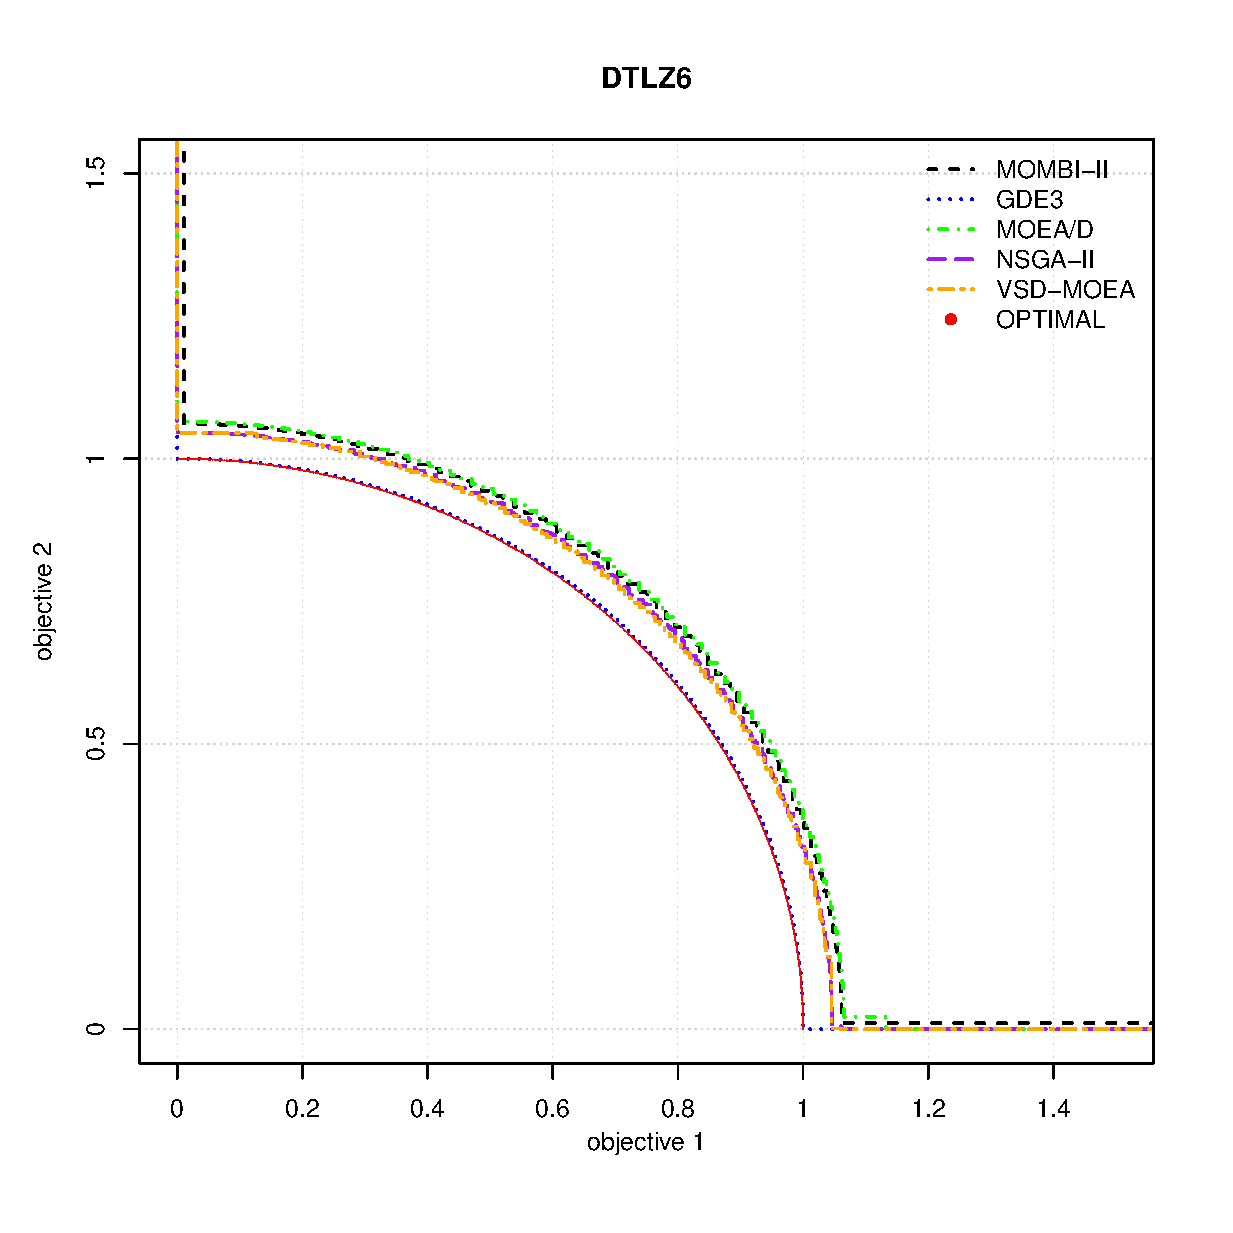
\includegraphics[width=0.33\textwidth]{Figures_Chapter7/Results_Chapter3/DTLZ6.eps}  &
  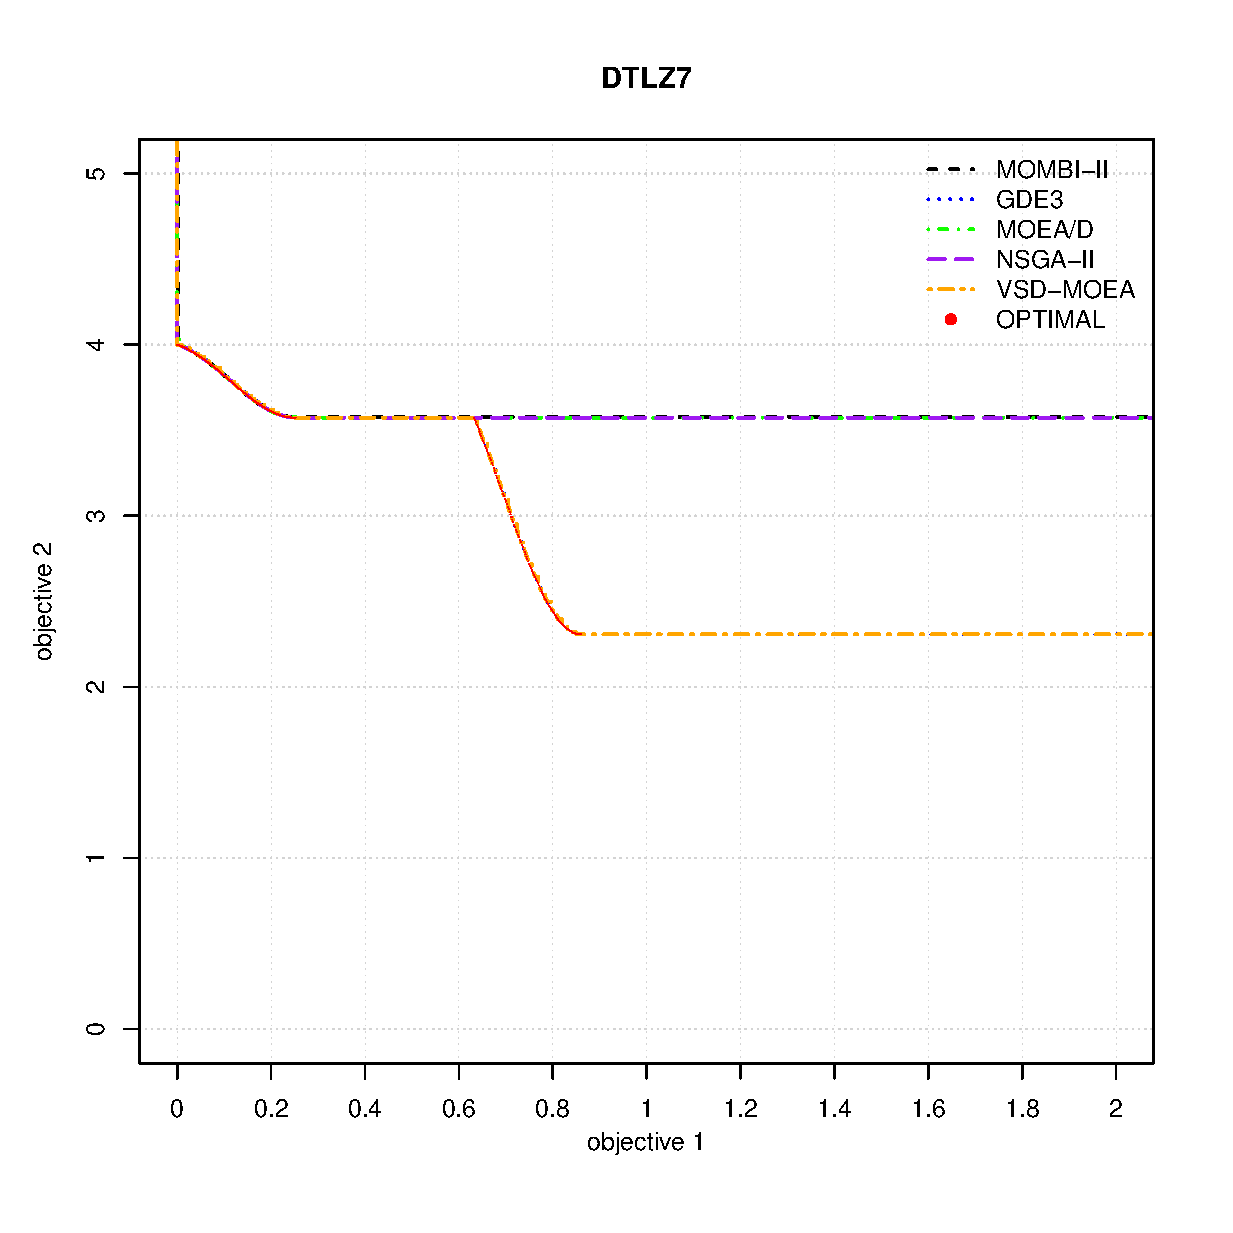
\includegraphics[width=0.33\textwidth]{Figures_Chapter7/Results_Chapter3/DTLZ7.eps} &
  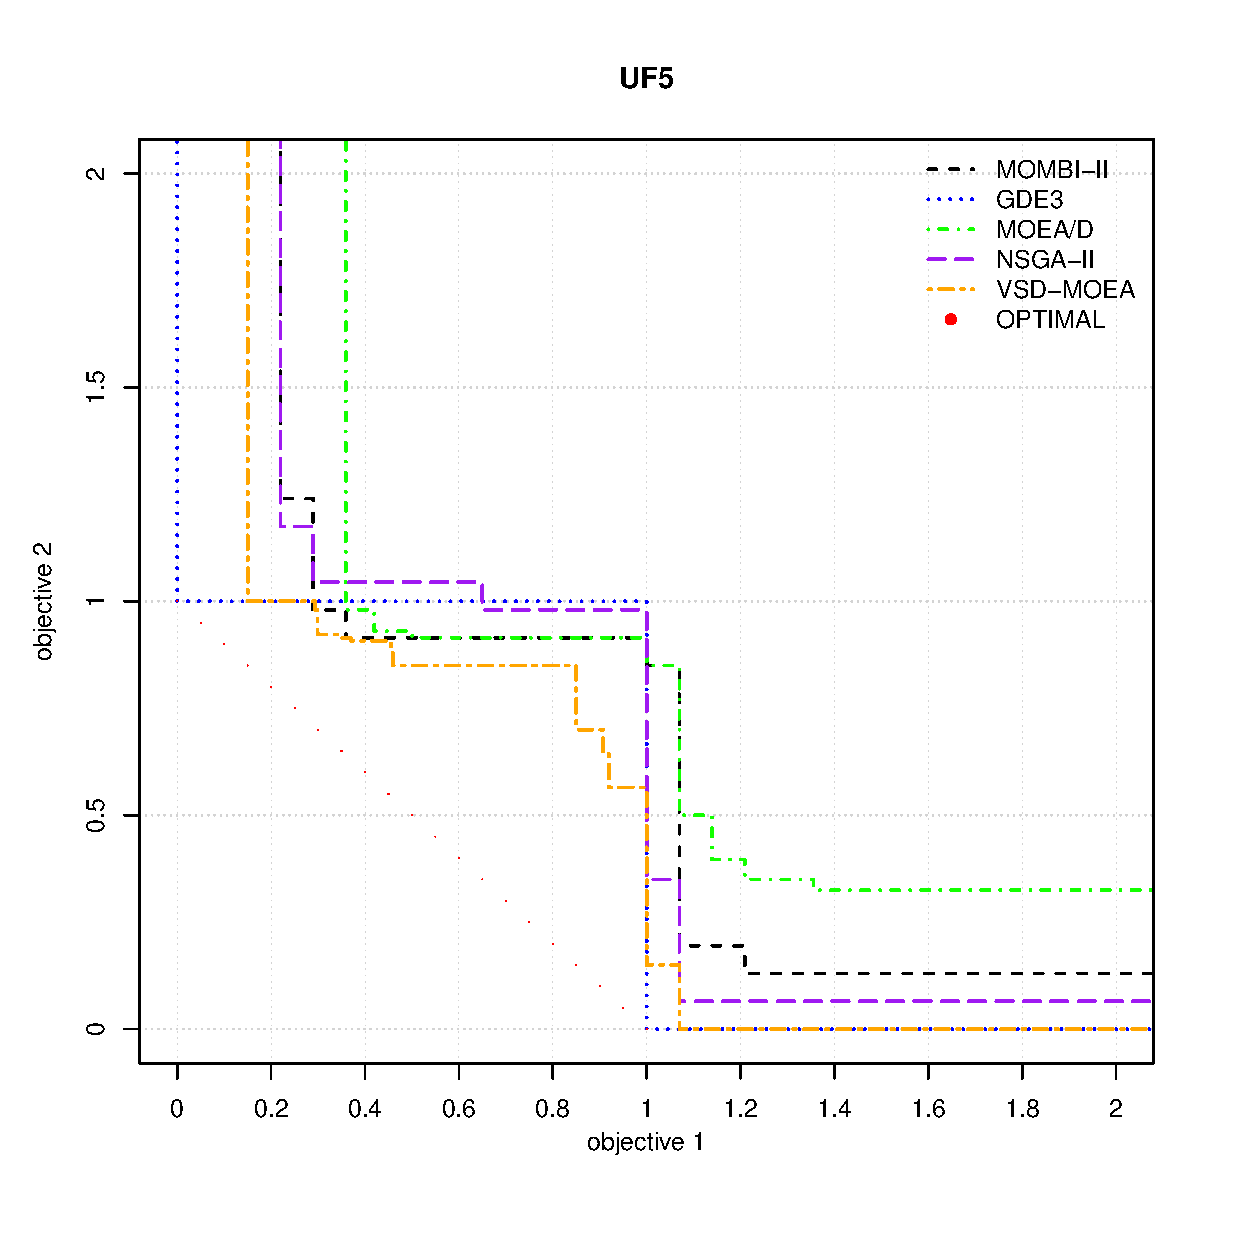
\includegraphics[width=0.33\textwidth]{Figures_Chapter7/Results_Chapter3/UF5.eps} \\
  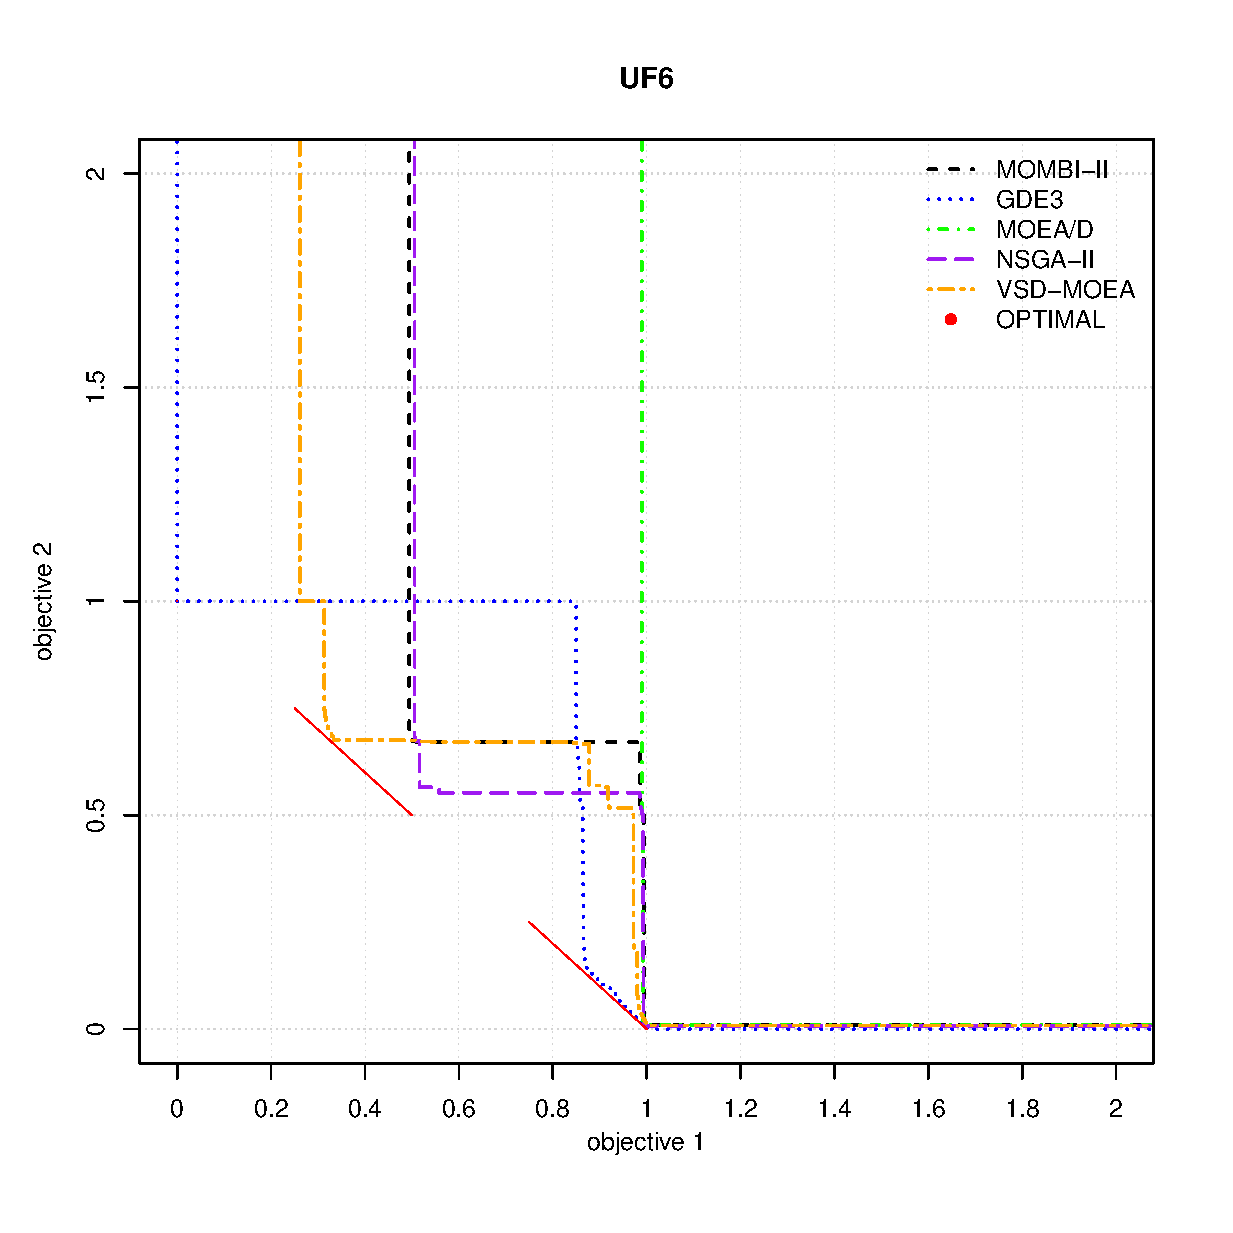
\includegraphics[width=0.33\textwidth]{Figures_Chapter7/Results_Chapter3/UF6.eps} &
  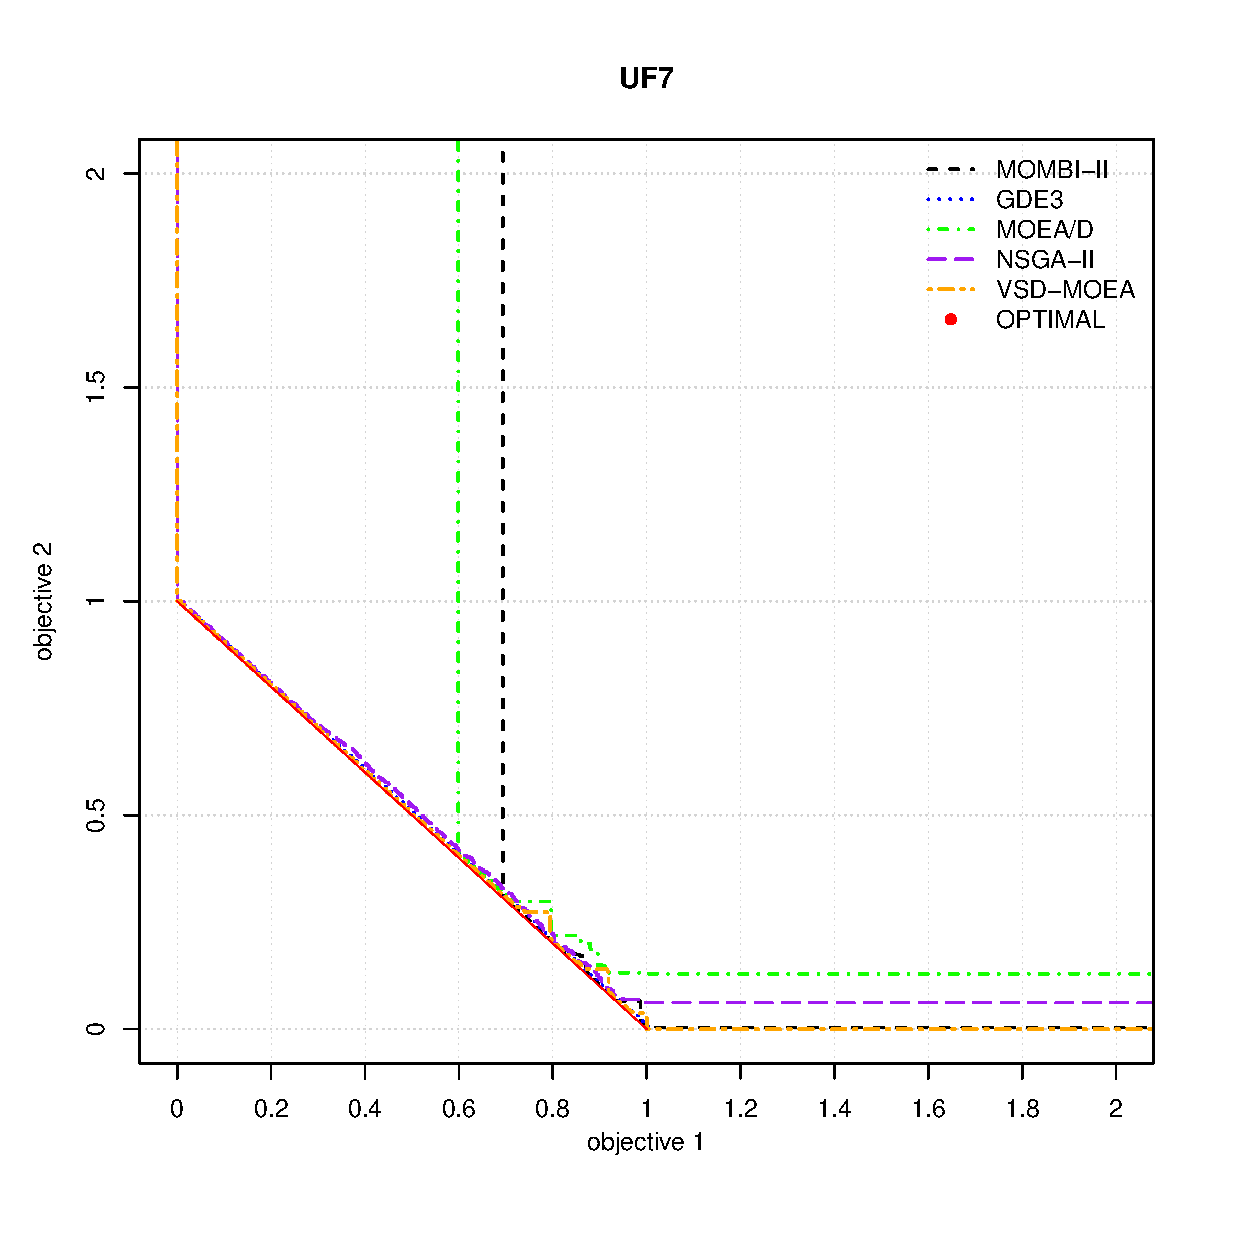
\includegraphics[width=0.33\textwidth]{Figures_Chapter7/Results_Chapter3/UF7.eps} &
  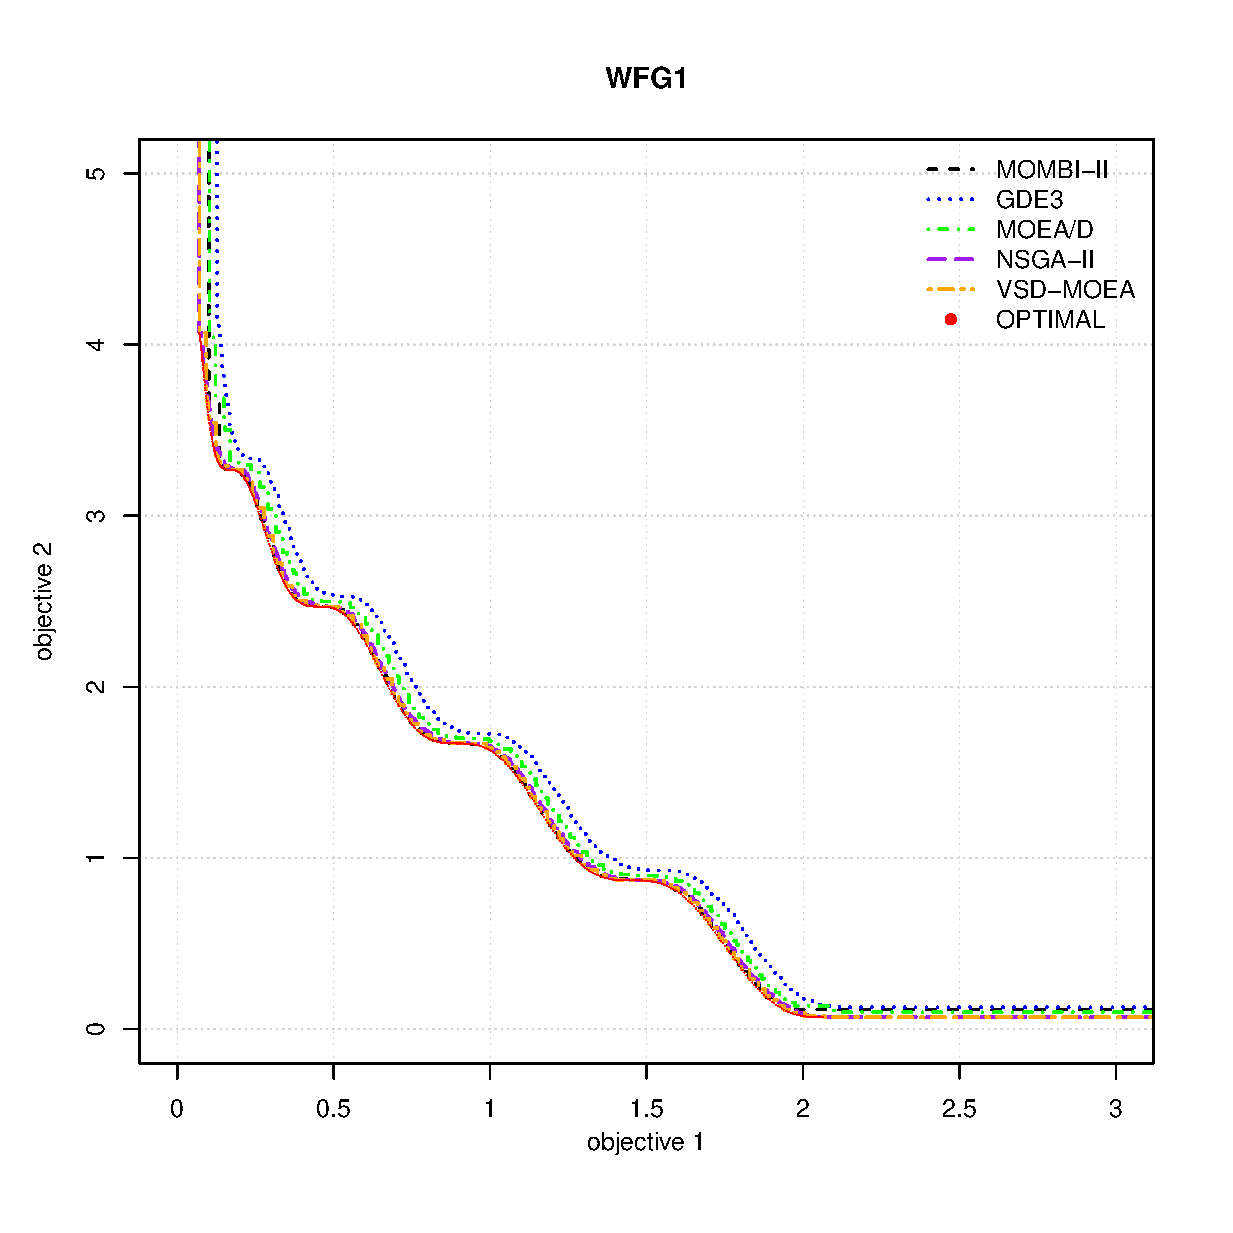
\includegraphics[width=0.33\textwidth]{Figures_Chapter7/Results_Chapter3/WFG1.eps} \\
  \includegraphics[width=0.33\textwidth]{Figures_Chapter7/Results_Chapter3/WFG2.eps} &
  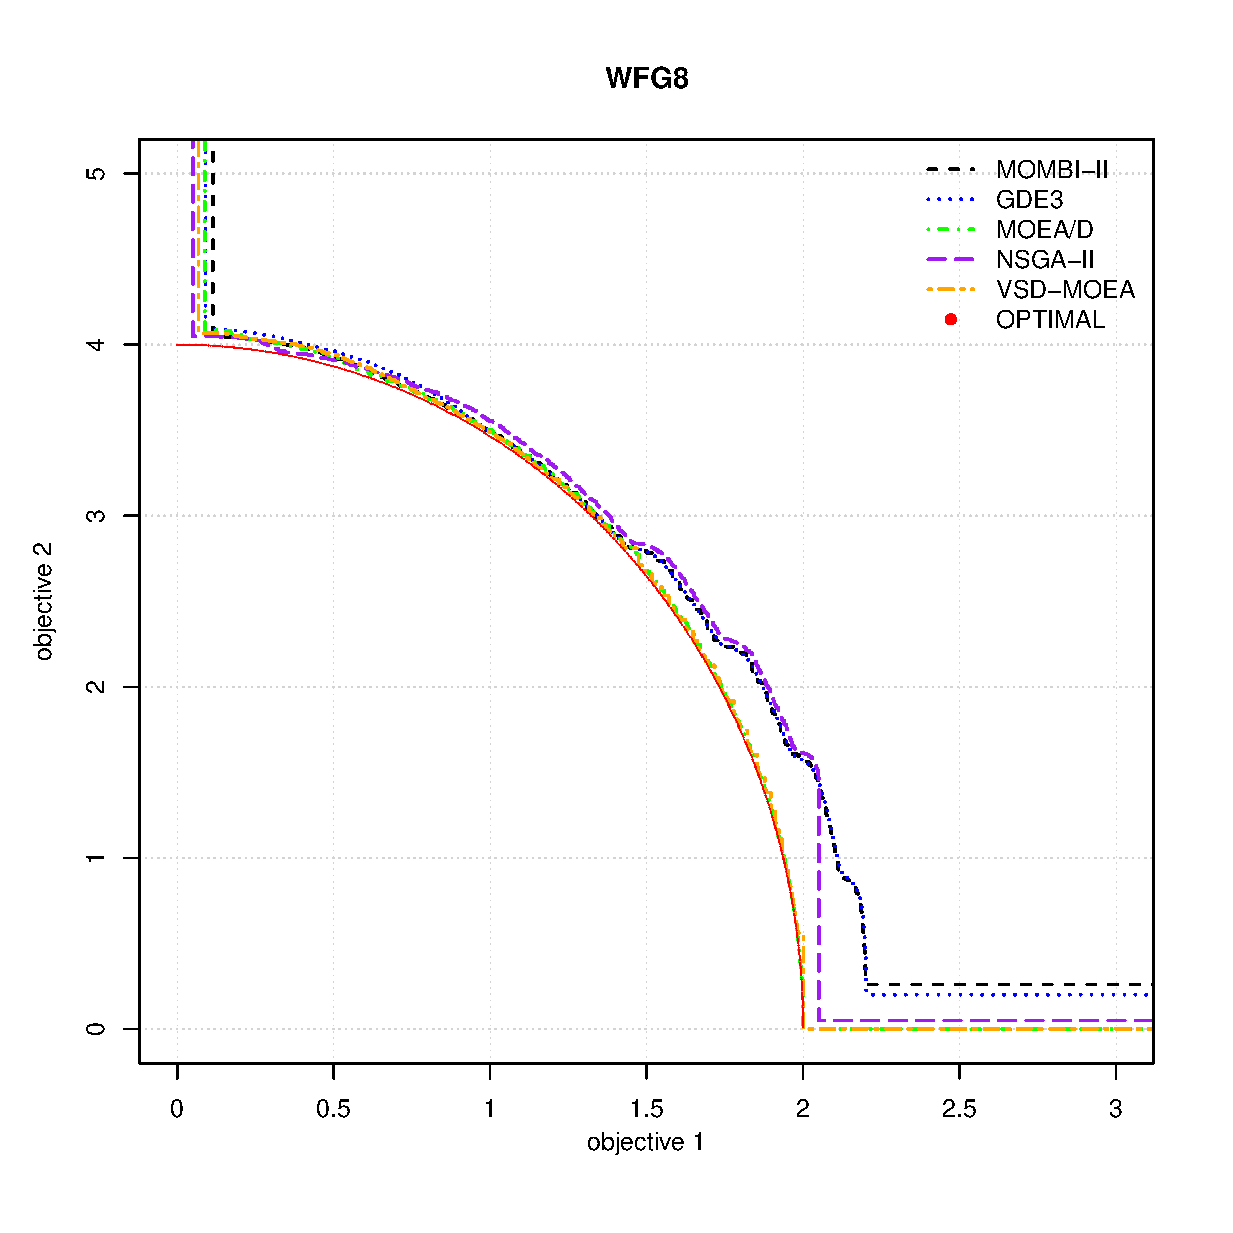
\includegraphics[width=0.33\textwidth]{Figures_Chapter7/Results_Chapter3/WFG8.eps} &
  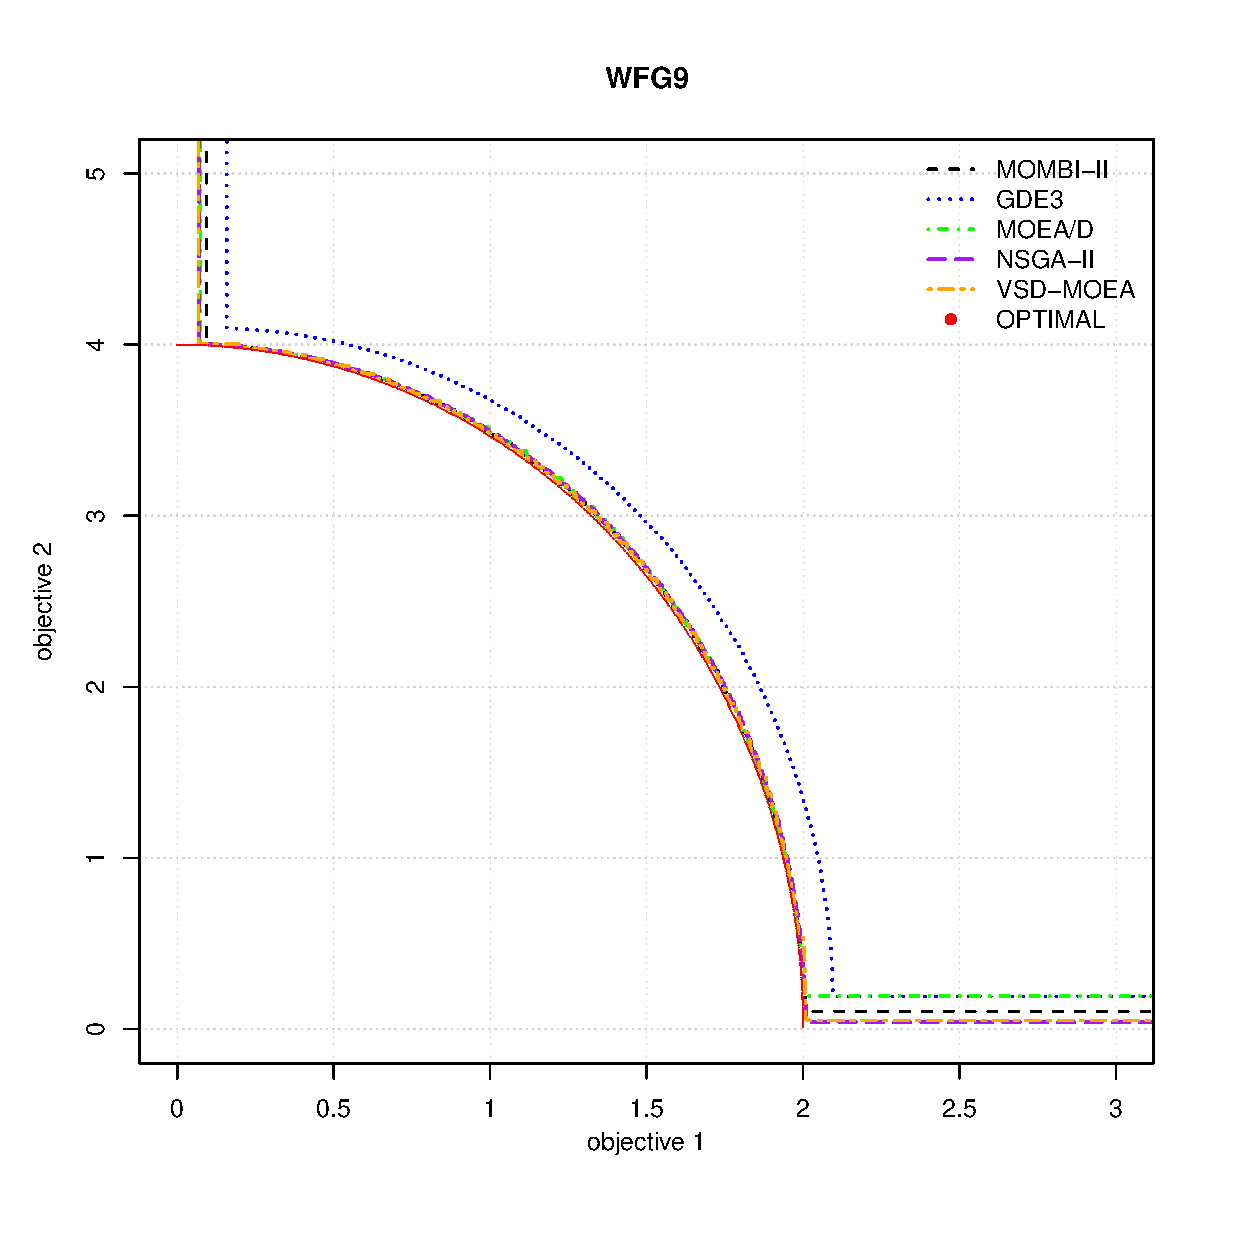
\includegraphics[width=0.33\textwidth]{Figures_Chapter7/Results_Chapter3/WFG9.eps}
\end{tabular}
\end{figure}
%


%----------------------------------------------------------------------------------------


\section{Algoritmos basados en descomposición}

\subsection{Validación experimental del MOEA/D-EVSD}

Esta sección está dedicada para validar el MOEA/D-EVSD, particularmente se utilizaron los nueve problemas de prueba WFG, el criterio de paro fue configurado a $50,000$ generaciones, el tamaño de la población fue fijado a $250$, y los problemas WFG fueron configurados con dos objetivos, el GDE3 fue configurado con los parámetros $C=0.5$ y $F=0.5$, el resto es indicado al inicio de este capítulo.
%
Nuestra análisis experimental se lleva de acuerdo a la superficies de cubrimiento logradas y al hipervolumen.
%
En cuatro de los problemas de prueba (WFG 3, 4, 5 y 7), todos lo métodos reportaron resultados bastantemente similares.
%
De hecho, la diferencias entre las medias del hipervolumen obtenido por los métodos fue menor que $0.1$.
%
Entonces, nuestro estudio se centra en los problemas restantes, sin embargo los resultados de estos problemas pueden ser consultados en el apéndice \ref{AppendixB}.
%
El 50\% de las superficies de cubrimiento logradas para los problemas WFG1, WFG2 y WFG8 son mostrados en la figura~\ref{Fig:AttainmentSurfaces_Mating}. 
%
Además, es trazado el frente de Pareto.
%
El análisis de esta figura muestra que las modificaciones introducidas en el MOEA/D provocan cambios significativos en los resultados.
%
Sin embargo, existen casos donde el MOEA/D-EVSD es significativamente mejor, mientras que en otros problemas existe una degradación en el rendimiento.
%
Los problemas WFG1 y WFG8 demuestran los beneficios ofrecidos por el MOEA/D-EVSD.
%
En tales casos, ninguno de los MOEAs que pertenecen al estado-del-arte proporcionaron resultados de mayor calidad.
%
Sin embargo, el MOEA/D-EVSD pudo obtener una aproximación buena del frente de Pareto.


El MOEA/D-EVSD tiene un peor comportamiento en relación a algunos MOEAs que pertenecen al estado-del-arte en los problemas WFG2, WFG6 y WFG9.
%
Particularmente, revisando el contenido de la población en estos casos, encontramos que, en cada individuo hijo del proceso de optimizacion, en el MOEA/D-EVSD algúnas de las variables de posición fueron muy elevadas o pequeñas en cada individuo.
%
La razón de esto, es debido a la forma en que la selección se realiza, hay una tendencia donde frecuentemente se seleccionan los individuos que presentan valores muy elevados o muy pequeños en sus variables.
%
Esta tendencia se origina ya que en el proceso de emparejamiento se seleccionan los individuos más distantes de este conjunto.
%
Por lo tanto, cuando hay individuos ubicados en lugares cercanos a los límites que pertenecen al espacio de las variables donde se presentan valores de calidad, éstos son seleccionados muy frecuentemente, entonces podría presentarse una convergencia prematura en éstas regiones.

%
Mientras nuestra propuesta ha sido útil para demostrar que incrementando la diversidad en el espacio de las variables es una forma para mejorar aún más los resultados en problemas que no son resueltos por los algoritmos que pertenecen al estado-del-arte, es introducida una tendencia de seleccionar individuos en ciertas zonas.
%
Por lo tanto, en la siguiente sección son analizadas otras formas para incrementar la diversidad de forma explícito.
%

Finalmente, en orden para validar completamente las conclusiones previas, se presenta un análisis del hipervolumen en las tablas \ref{table:StatisticalTest_Mating} y \ref{table:Statistics_Mating}.
%
La tabla \ref{table:Statistics_Mating} muestra el mínimo, máximo, media y la desviación estándar del hipervolumen obtenido por los distintos optimizadores probados.
%
El punto de referencia fue establecido en $(3.0, 5.0)$ (\cite{Joel:OperatorAHX}). 
%
Adicionalmente, se realizaron pruebas estadísticas por pares (Tabla~\ref{table:StatisticalTest_Mating}).
%
%Para cada instancia, la columna ''$\uparrow$'' reporta el número de comparaciones donde las pruebas estadísticas confirman superioridad del AEMO listado en la fila correspondiente, mientras que la columna ''$\downarrow$'' reporta el número de casos donde éste fue inferior.
%
Los valores obtenidos con el hipervolumen y las pruebas estadísticas correspondientes confirman la superioridad del MOEA/D-EVSD en los problemas WFG1 y WFG8.
%
De hecho, la pruebas estadísticas confirman en ambos casos que el MOEA/D-EVSD es superior a los MOEAs restantes.
%
Sin embargo, como se explicó anteriormente, las pruebas también confirman la inferioridad del MOEA/D-EVSD en los casos restantes.
  
 
 % Please add the following required packages to your document preamble:
% \usepackage{graphicx}
\begin{table}[]
\centering
\scriptsize
\caption{Pruebas Estadísticas del Hipervolumen}
\label{table:StatisticalTest_Mating}
%\resizebox{\textwidth}{!}{%
\begin{tabular}{c|c|c|c|c|c|c|c|c|c|c|}
\cline{2-11}
\multicolumn{1}{l|}{} & \multicolumn{2}{c|}{WFG1} & \multicolumn{2}{c|}{WFG2} & \multicolumn{2}{c|}{WFG6} & \multicolumn{2}{c|}{WFG8} & \multicolumn{2}{c|}{WFG9} \\ \cline{2-11} 
\multicolumn{1}{l|}{} & $\uparrow$ & $\downarrow$ & $\uparrow$ & $\downarrow$ & $\uparrow$ & $\downarrow$ & $\uparrow$ & $\downarrow$ & $\uparrow$ & $\downarrow$ \\ \hline
\multicolumn{1}{|c|}{MOEA/D-EVSD} & 4 & 0 & 3 & 1 & 0 & 4 & 4 & 0 & 0 & 4 \\ \hline
\multicolumn{1}{|c|}{GDE3} & 3 & 1 & 4 & 0 & 4 & 0 & 3 & 1 & 1 & 3 \\ \hline
\multicolumn{1}{|c|}{MOEA/D} & 1 & 2 & 0 & 4 & 1 & 1 & 2 & 2 & 3 & 0 \\ \hline
\multicolumn{1}{|c|}{NSGAII} & 1 & 2 & 1 & 2 & 1 & 1 & 0 & 4 & 2 & 2 \\ \hline
\multicolumn{1}{|c|}{SMS-EMOA} & 0 & 4 & 1 & 2 & 1 & 1 & 1 & 3 & 3 & 0 \\ \hline
\end{tabular}%
%}
\end{table}
   

% Please add the following required packages to your document preamble:
% \usepackage{graphicx}
\begin{table*}[]
\centering
\scriptsize
\caption{Estadísticas del Hipervolumen}
\label{table:Statistics_Mating}
\resizebox{\textwidth}{!}{%
\begin{tabular}{ccccccccccccccccccccc}
\cline{2-21}
\multicolumn{1}{c|}{} & \multicolumn{4}{c|}{MOEA/D-EVSD} & \multicolumn{4}{c|}{GDE3} & \multicolumn{4}{c|}{MOEA/D} & \multicolumn{4}{c|}{NSGAII} & \multicolumn{4}{c|}{SMS-EMOA} \\ \hline
\multicolumn{1}{|c|}{} & \multicolumn{1}{c|}{Min} & \multicolumn{1}{c|}{Max} & \multicolumn{1}{c|}{Media} & \multicolumn{1}{c|}{SD} & \multicolumn{1}{c|}{Min} & \multicolumn{1}{c|}{Max} & \multicolumn{1}{c|}{Media} & \multicolumn{1}{c|}{SD} & \multicolumn{1}{c|}{Min} & \multicolumn{1}{c|}{Max} & \multicolumn{1}{c|}{Media} & \multicolumn{1}{c|}{SD} & \multicolumn{1}{c|}{Min} & \multicolumn{1}{c|}{Max} & \multicolumn{1}{c|}{Media} & \multicolumn{1}{c|}{SD} & \multicolumn{1}{c|}{Min} & \multicolumn{1}{c|}{Max} & \multicolumn{1}{c|}{Media} & \multicolumn{1}{c|}{SD} \\ \hline
\multicolumn{1}{|c|}{WFG1} & \multicolumn{1}{c|}{11.53} & \multicolumn{1}{c|}{11.54} & \multicolumn{1}{c|}{\textbf{11.54}} & \multicolumn{1}{c|}{2.02E-03} & \multicolumn{1}{c|}{10.90} & \multicolumn{1}{c|}{11.40} & \multicolumn{1}{c|}{11.12} & \multicolumn{1}{c|}{1.50E-01} & \multicolumn{1}{c|}{9.63} & \multicolumn{1}{c|}{10.68} & \multicolumn{1}{c|}{10.36} & \multicolumn{1}{c|}{2.63E-01} & \multicolumn{1}{c|}{10.11} & \multicolumn{1}{c|}{10.65} & \multicolumn{1}{c|}{10.38} & \multicolumn{1}{c|}{2.21E-01} & \multicolumn{1}{c|}{9.51} & \multicolumn{1}{c|}{10.09} & \multicolumn{1}{c|}{9.89} & \multicolumn{1}{c|}{2.42E-01} \\ \hline
\multicolumn{1}{|c|}{WFG2} & \multicolumn{1}{c|}{10.62} & \multicolumn{1}{c|}{11.46} & \multicolumn{1}{c|}{10.89} & \multicolumn{1}{c|}{3.88E-01} & \multicolumn{1}{c|}{11.47} & \multicolumn{1}{c|}{11.47} & \multicolumn{1}{c|}{\textbf{11.47}} & \multicolumn{1}{c|}{4.75E-05} & \multicolumn{1}{c|}{10.63} & \multicolumn{1}{c|}{10.63} & \multicolumn{1}{c|}{10.63} & \multicolumn{1}{c|}{2.53E-04} & \multicolumn{1}{c|}{10.63} & \multicolumn{1}{c|}{10.63} & \multicolumn{1}{c|}{10.63} & \multicolumn{1}{c|}{2.73E-04} & \multicolumn{1}{c|}{10.63} & \multicolumn{1}{c|}{10.63} & \multicolumn{1}{c|}{10.63} & \multicolumn{1}{c|}{5.75E-04} \\ \hline
\multicolumn{1}{|c|}{WFG6} & \multicolumn{1}{c|}{7.99} & \multicolumn{1}{c|}{8.11} & \multicolumn{1}{c|}{8.05} & \multicolumn{1}{c|}{3.01E-02} & \multicolumn{1}{c|}{8.60} & \multicolumn{1}{c|}{8.65} & \multicolumn{1}{c|}{\textbf{8.61}} & \multicolumn{1}{c|}{2.06E-02} & \multicolumn{1}{c|}{7.81} & \multicolumn{1}{c|}{8.50} & \multicolumn{1}{c|}{8.35} & \multicolumn{1}{c|}{1.30E-01} & \multicolumn{1}{c|}{8.31} & \multicolumn{1}{c|}{8.44} & \multicolumn{1}{c|}{8.37} & \multicolumn{1}{c|}{3.60E-02} & \multicolumn{1}{c|}{8.28} & \multicolumn{1}{c|}{8.48} & \multicolumn{1}{c|}{8.39} & \multicolumn{1}{c|}{4.23E-02} \\ \hline
\multicolumn{1}{|c|}{WFG8} & \multicolumn{1}{c|}{7.96} & \multicolumn{1}{c|}{8.60} & \multicolumn{1}{c|}{\textbf{8.44}} & \multicolumn{1}{c|}{2.39E-01} & \multicolumn{1}{c|}{7.93} & \multicolumn{1}{c|}{7.94} & \multicolumn{1}{c|}{7.93} & \multicolumn{1}{c|}{3.97E-03} & \multicolumn{1}{c|}{7.83} & \multicolumn{1}{c|}{7.89} & \multicolumn{1}{c|}{7.87} & \multicolumn{1}{c|}{1.85E-02} & \multicolumn{1}{c|}{7.82} & \multicolumn{1}{c|}{7.86} & \multicolumn{1}{c|}{7.84} & \multicolumn{1}{c|}{1.01E-02} & \multicolumn{1}{c|}{7.82} & \multicolumn{1}{c|}{7.89} & \multicolumn{1}{c|}{7.86} & \multicolumn{1}{c|}{1.73E-02} \\ \hline
\multicolumn{1}{|c|}{WFG9} & \multicolumn{1}{c|}{7.72} & \multicolumn{1}{c|}{8.21} & \multicolumn{1}{c|}{7.73} & \multicolumn{1}{c|}{8.21E-02} & \multicolumn{1}{c|}{7.72} & \multicolumn{1}{c|}{7.79} & \multicolumn{1}{c|}{7.75} & \multicolumn{1}{c|}{2.27E-02} & \multicolumn{1}{c|}{7.72} & \multicolumn{1}{c|}{8.57} & \multicolumn{1}{c|}{\textbf{8.30}} & \multicolumn{1}{c|}{2.43E-01} & \multicolumn{1}{c|}{7.72} & \multicolumn{1}{c|}{8.58} & \multicolumn{1}{c|}{7.82} & \multicolumn{1}{c|}{2.71E-01} & \multicolumn{1}{c|}{7.72} & \multicolumn{1}{c|}{8.58} & \multicolumn{1}{c|}{8.21} & \multicolumn{1}{c|}{3.59E-01} \\ \hline
\multicolumn{1}{l}{} & \multicolumn{1}{l}{} & \multicolumn{1}{l}{} & \multicolumn{1}{l}{} & \multicolumn{1}{l}{} & \multicolumn{1}{l}{} & \multicolumn{1}{l}{} & \multicolumn{1}{l}{} & \multicolumn{1}{l}{} & \multicolumn{1}{l}{} & \multicolumn{1}{l}{} & \multicolumn{1}{l}{} & \multicolumn{1}{l}{} & \multicolumn{1}{l}{} & \multicolumn{1}{l}{} & \multicolumn{1}{l}{} & \multicolumn{1}{l}{} & \multicolumn{1}{l}{} & \multicolumn{1}{l}{} & \multicolumn{1}{l}{} & \multicolumn{1}{l}{}
\end{tabular}%
}
\end{table*}

\begin{figure}[H]
%%\centering
\caption{superficies de cubrimiento logradas al 50\%}%Attainment Figures\_Chapter7 Achieved}
\label{Fig:AttainmentSurfaces_Mating}
\begin{tabular}{ccc}
  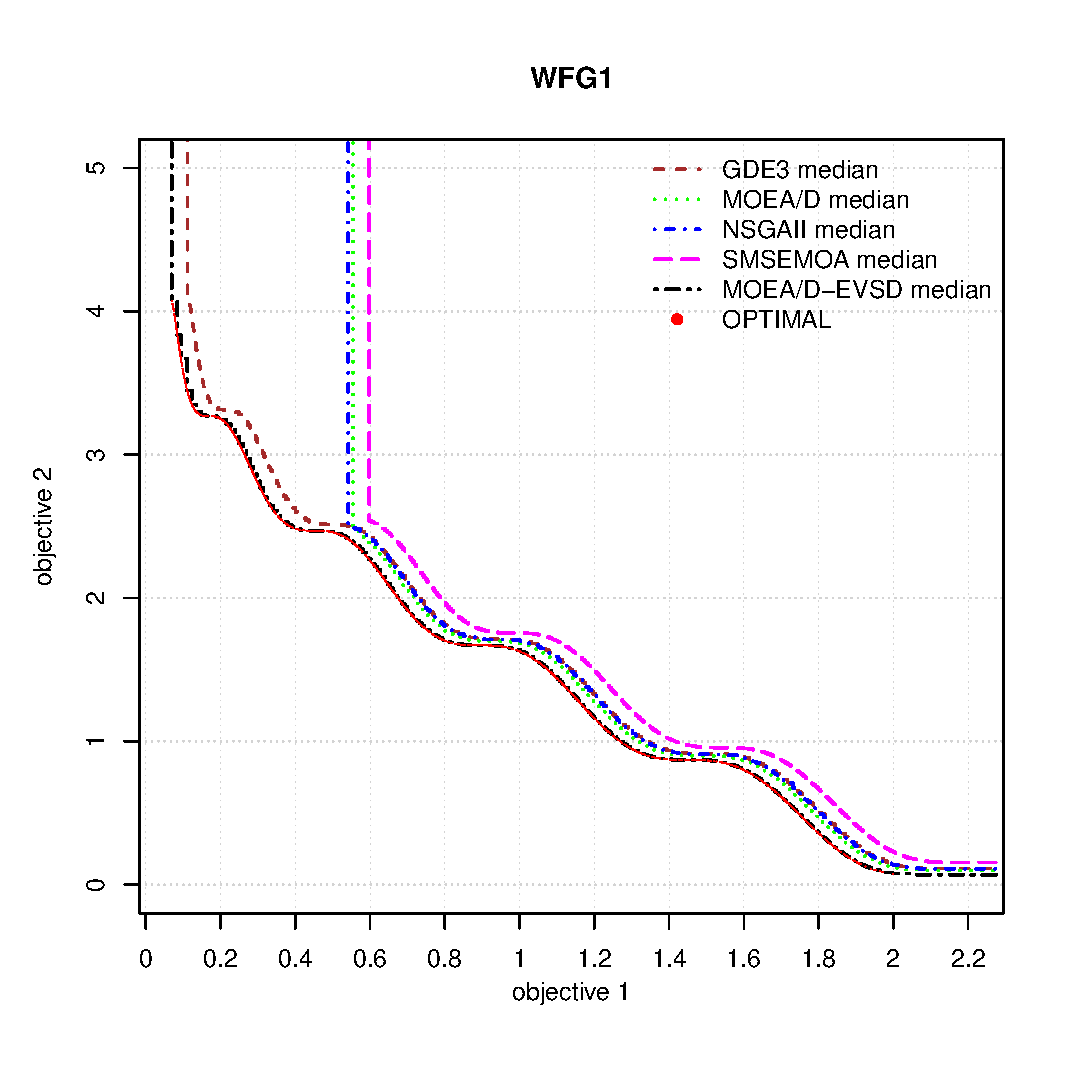
\includegraphics[width=0.33\textwidth]{Figures_Chapter7/Results_Chapter4/Surface_eps/WFG1.eps}  &
  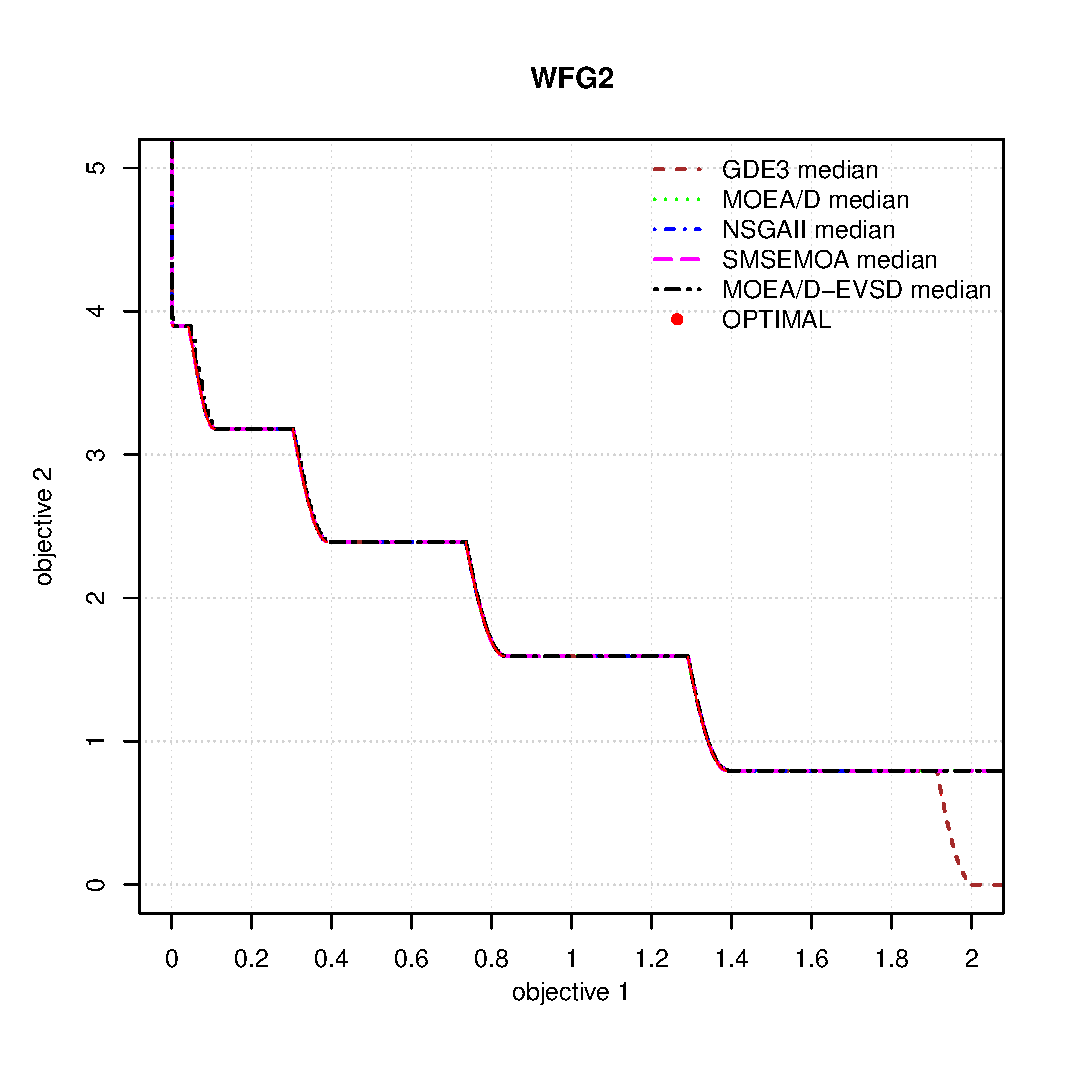
\includegraphics[width=0.33\textwidth]{Figures_Chapter7/Results_Chapter4/Surface_eps/WFG2.eps}  &
  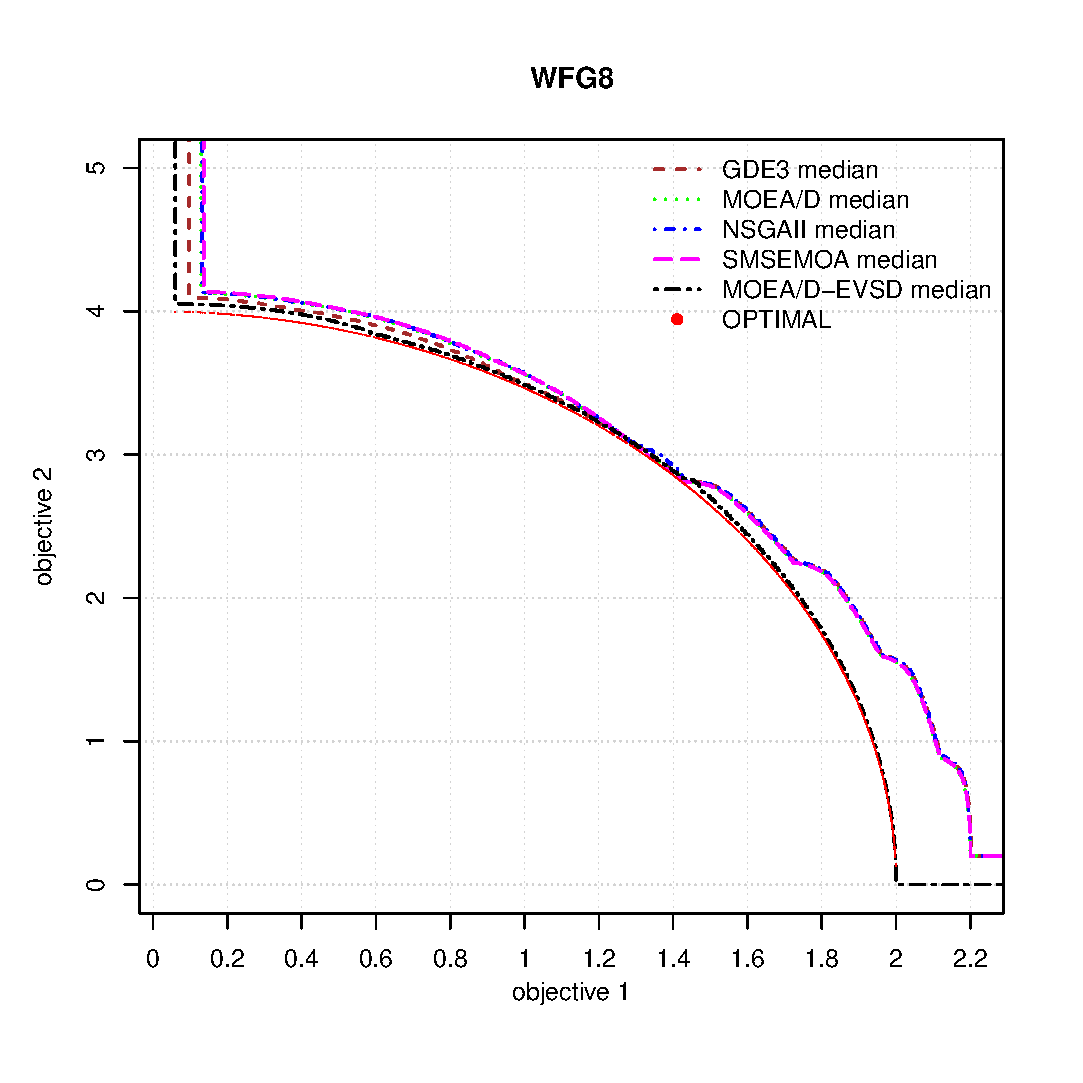
\includegraphics[width=0.33\textwidth]{Figures_Chapter7/Results_Chapter4/Surface_eps/WFG8.eps} 
\end{tabular}
\end{figure}

\subsection{Validación experimental de los algoritmos MOEA/D-SEBV y VSD-MOEA/D}

En esta sección se validan experimentalmente las dos propuestas para promover la diversidad de forma explícita y que son basados en descomposición.
%
En las tablas \ref{tab:IGD_Estadisticas_IGD_VSD_MOEA_D}, \ref{tab:IGD_Estadisticas_HV_VSD_MOEA_D} son consideradas cuatro versiones del VSD-MOEA/D, con el propósito de observar el comportamiento con diferentes configuraciones.
%
Inicialmente, se seleccionan los algoritmos \textit{MOEA/D-SEBV} y \textit{VSD-MOEA/D Normal DE}, los cuales implementan el enfoque de Tchebycheff y un factor de mutación $CR=0.9$.
%
El resto de algoritmos implementan las modificaciones a DE sugeridas en el capítulo \ref{Chapter5}, donde no es requerido un factor de mutación y además aplican el enfoque basado en la función de escalarización aumentada (ASFA) propuesta en el capítulo \ref{Chapter4}.
%
Por su parte los algoritmos \textit{Fast VSD-MOEA/D} y \textit{MOEA/D-VSD T=10} están configurados con un tamaño de vecindad $T=10$.
%
Se recuerda que el \textit{Fast VSD-MOEA/D}, es la versión optimizada del \textit{MOEA/D-VSD}.
%
Con el propósito de observar el efecto que tiene el tamaño de las vecindades se agrega el \textit{MOEA/D-VSD T=100}.
%
Específicamente, son analizados el IGD+ en dos objetivos y el hipervolumen con tres objetivos, el resto de material se puede consultar en el apéndice \ref{AppendixB}.

Principalmente, se observa que considerando dos objetivos, el MOEA/D-SEBV no es mejor en ninguna instancia que el resto de algoritmos, además los peores resultados con este algoritmo son encontrados en las instancias UF4, UF5 y WFG8.
%
Especialmente, el conjunto óptimo de las instancias UF4 y UF5 corresponde a secciones aisladas en el espacio factible, por lo tanto es necesario que el operador sea rotacionalemente invariante, en consecuencia son proporcionados los peores resultados por los algoritmos \textit{MOEA/D-SEBV} y el \textit{VSD-MOEA/D Normal DE} por el factor de mutación que utilizan.

Además, es importante notar que en la mayoría de instancias no existe un efecto significativo en el tamaño de las vecindades,  \textit{MOEA/D-VSD T=10} y \textit{MOEA/D-VSD T=100}.

Por otra parte, el \textit{Fast VSD-MOEA/D} proporciona resultados cercanos al \textit{VSD-MOEA/D T=10} e inclusive mejores en las instancias WFG8 y WFG9, esto se debe a que estas instancias poseen un grado de dependencia entre los parámetros, así el esquema que utiliza el primer algoritmo no considera al vecino más cercano, en su lugar, se enfoca en la diversidad de la población, por lo tanto en algunos casos se podrían seleccionar dos individuos cercanos, pero cuya contribución a la diversidad es suficiente.

Se puede observar, que conforme aumenta el número de objetivos, las propuestas que utilizan una factor de mutación fijo (\textit{MOEA/D-SEBV} y \textit{VSD-MOEA/D Normal DE}) son degradados, principalmente en la instancia WFG1, que como ya se ha mencionado, esta instancia es separable en los parámetros y por lo tanto se requiere un factor de mutación ($CR$) pequeño.

%
Adicionalmente, analizando los resultados de las instancias UF8, UF9 y UF10, se observa el efecto de utilizar el enfoque de escalarización aumentado (ASFA), este enfoque puede proporcionar resultados ligeramente inferiores en instancias sencillas, como es el caso del DTLZ1, esto sucede ya que la distribución de la soluciones es diferente al ser un enfoque que produce soluciones fuertemente dominantes, afectando las regiones planas del frente de Pareto.


En base a los resultados obtenidos, se puede concluir que los cambios propuestos de DE producen un comportamiento más estable en esquemas de diversidad a largo plazo, además el indicador propuesto (ASFA) ofrece mejores resultados en instancias difíciles.

% Please add the following required packages to your document preamble:
% \usepackage{graphicx}
\begin{table}[H]
\centering
\caption{Estadísticas IGD+ considerando dos objetivos}
\label{tab:IGD_Estadisticas_IGD_VSD_MOEA_D}
\resizebox{\textwidth}{!}{%
\begin{tabular}{c|c|c|c|c|c|c|c|c|c|c|c|c|c|c|c|}
\cline{2-16}
 & \multicolumn{3}{c|}{MOEA/D-SEBV} & \multicolumn{3}{c|}{VSD-MOEA/D T=10} & \multicolumn{3}{c|}{VSD-MOEA/D T=100} & \multicolumn{3}{c|}{VSD-MOEA/D Normal DE} & \multicolumn{3}{c|}{Fast VSD-MOEA/D} \\ \cline{2-16} 
 & Min & Max & Mean & Min & Max & Mean & Min & Max & Mean & Min & Max & Mean & Min & Max & Mean \\ \hline
\multicolumn{1}{|c|}{DTLZ1} & 0.001 & 0.001 & \textbf{0.001} & 0.001 & 0.001 & \textbf{0.001} & 0.001 & 0.001 & \textbf{0.001} & 0.001 & 0.001 & \textbf{0.001} & 0.001 & 0.001 & \textbf{0.001} \\ \hline
\multicolumn{1}{|c|}{DTLZ2} & 0.002 & 0.002 & \textbf{0.002} & 0.002 & 0.002 & \textbf{0.002} & 0.002 & 0.002 & \textbf{0.002} & 0.002 & 0.002 & \textbf{0.002} & 0.002 & 0.002 & \textbf{0.002} \\ \hline
\multicolumn{1}{|c|}{DTLZ3} & 0.002 & 0.002 & \textbf{0.002} & 0.002 & 0.002 & \textbf{0.002} & 0.002 & 0.002 & \textbf{0.002} & 0.002 & 0.002 & \textbf{0.002} & 0.002 & 0.002 & \textbf{0.002} \\ \hline
\multicolumn{1}{|c|}{DTLZ4} & 0.002 & 0.363 & 0.033 & 0.002 & 0.002 & \textbf{0.002} & 0.002 & 0.002 & \textbf{0.002} & 0.002 & 0.002 & \textbf{0.002} & 0.002 & 0.002 & \textbf{0.002} \\ \hline
\multicolumn{1}{|c|}{DTLZ5} & 0.002 & 0.002 & \textbf{0.002} & 0.002 & 0.002 & \textbf{0.002} & 0.002 & 0.002 & \textbf{0.002} & 0.002 & 0.002 & \textbf{0.002} & 0.002 & 0.002 & \textbf{0.002} \\ \hline
\multicolumn{1}{|c|}{DTLZ6} & 0.002 & 0.002 & \textbf{0.002} & 0.002 & 0.002 & \textbf{0.002} & 0.002 & 0.002 & \textbf{0.002} & 0.002 & 0.002 & \textbf{0.002} & 0.002 & 0.002 & \textbf{0.002} \\ \hline
\multicolumn{1}{|c|}{DTLZ7} & 0.003 & 0.003 & \textbf{0.003} & 0.003 & 0.003 & \textbf{0.003} & 0.003 & 0.003 & \textbf{0.003} & 0.003 & 0.003 & \textbf{0.003} & 0.003 & 0.003 & \textbf{0.003} \\ \hline
\multicolumn{1}{|c|}{UF1} & 0.003 & 0.003 & \textbf{0.003} & 0.003 & 0.003 & \textbf{0.003} & 0.002 & 0.003 & \textbf{0.003} & 0.003 & 0.003 & \textbf{0.003} & 0.002 & 0.003 & \textbf{0.003} \\ \hline
\multicolumn{1}{|c|}{UF2} & 0.004 & 0.004 & 0.004 & 0.003 & 0.003 & \textbf{0.003} & 0.003 & 0.003 & \textbf{0.003} & 0.004 & 0.004 & 0.004 & 0.003 & 0.003 & \textbf{0.003} \\ \hline
\multicolumn{1}{|c|}{UF3} & 0.003 & 0.036 & 0.007 & 0.002 & 0.002 & \textbf{0.002} & 0.003 & 0.007 & 0.003 & 0.003 & 0.003 & 0.003 & 0.003 & 0.003 & 0.003 \\ \hline
\multicolumn{1}{|c|}{UF4} & 0.042 & 0.050 & 0.045 & 0.023 & 0.026 & \textbf{0.024} & 0.024 & 0.026 & 0.025 & 0.033 & 0.037 & 0.035 & 0.023 & 0.026 & 0.025 \\ \hline
\multicolumn{1}{|c|}{UF5} & 0.006 & 0.040 & 0.036 & 0.000 & 0.005 & \textbf{0.000} & 0.000 & 0.000 & \textbf{0.000} & 0.015 & 0.040 & 0.030 & 0.000 & 0.000 & \textbf{0.000} \\ \hline
\multicolumn{1}{|c|}{UF6} & 0.002 & 0.018 & 0.003 & 0.002 & 0.002 & \textbf{0.002} & 0.002 & 0.002 & \textbf{0.002} & 0.002 & 0.002 & \textbf{0.002} & 0.002 & 0.002 & \textbf{0.002} \\ \hline
\multicolumn{1}{|c|}{UF7} & 0.003 & 0.003 & \textbf{0.003} & 0.003 & 0.003 & \textbf{0.003} & 0.003 & 0.003 & \textbf{0.003} & 0.003 & 0.003 & \textbf{0.003} & 0.003 & 0.003 & \textbf{0.003} \\ \hline
\multicolumn{1}{|c|}{WFG1} & 0.007 & 0.122 & 0.028 & 0.007 & 0.046 & \textbf{0.013} & 0.007 & 0.059 & 0.017 & 0.007 & 0.108 & 0.027 & 0.007 & 0.048 & 0.015 \\ \hline
\multicolumn{1}{|c|}{WFG2} & 0.006 & 0.006 & \textbf{0.006} & 0.006 & 0.006 & \textbf{0.006} & 0.006 & 0.006 & \textbf{0.006} & 0.006 & 0.006 & \textbf{0.006} & 0.006 & 0.006 & \textbf{0.006} \\ \hline
\multicolumn{1}{|c|}{WFG3} & 0.008 & 0.008 & \textbf{0.008} & 0.008 & 0.008 & \textbf{0.008} & 0.008 & 0.008 & \textbf{0.008} & 0.008 & 0.008 & \textbf{0.008} & 0.008 & 0.008 & \textbf{0.008} \\ \hline
\multicolumn{1}{|c|}{WFG4} & 0.007 & 0.007 & \textbf{0.007} & 0.007 & 0.007 & \textbf{0.007} & 0.007 & 0.007 & \textbf{0.007} & 0.007 & 0.007 & \textbf{0.007} & 0.007 & 0.007 & \textbf{0.007} \\ \hline
\multicolumn{1}{|c|}{WFG5} & 0.064 & 0.069 & 0.067 & 0.061 & 0.070 & 0.066 & 0.061 & 0.069 & \textbf{0.065} & 0.064 & 0.069 & 0.068 & 0.059 & 0.070 & \textbf{0.065} \\ \hline
\multicolumn{1}{|c|}{WFG6} & 0.007 & 0.121 & 0.072 & 0.007 & 0.012 & \textbf{0.007} & 0.007 & 0.007 & \textbf{0.007} & 0.007 & 0.031 & 0.009 & 0.007 & 0.007 & \textbf{0.007} \\ \hline
\multicolumn{1}{|c|}{WFG7} & 0.007 & 0.007 & \textbf{0.007} & 0.007 & 0.007 & \textbf{0.007} & 0.007 & 0.007 & \textbf{0.007} & 0.007 & 0.007 & \textbf{0.007} & 0.007 & 0.007 & \textbf{0.007} \\ \hline
\multicolumn{1}{|c|}{WFG8} & 0.092 & 0.097 & 0.094 & 0.011 & 0.039 & 0.018 & 0.009 & 0.016 & \textbf{0.012} & 0.011 & 0.021 & 0.018 & 0.009 & 0.017 & \textbf{0.012} \\ \hline
\multicolumn{1}{|c|}{WFG9} & 0.011 & 0.126 & 0.062 & 0.010 & 0.012 & 0.012 & 0.009 & 0.013 & \textbf{0.011} & 0.009 & 0.012 & \textbf{0.011} & 0.010 & 0.013 & \textbf{0.011} \\ \hline
\end{tabular}%
}
\end{table}



% Please add the following required packages to your document preamble:
% \usepackage{graphicx}
\begin{table}[H]
\centering
\caption{Estadísticas del hipervolumen considerando tres objetivos}
\label{tab:IGD_Estadisticas_HV_VSD_MOEA_D}
\resizebox{\textwidth}{!}{%
\begin{tabular}{c|c|c|c|c|c|c|c|c|c|c|c|c|c|c|c|}
\cline{2-16}
 & \multicolumn{3}{c|}{MOEA/D-SEBV} & \multicolumn{3}{c|}{VSD-MOEA/D T=10} & \multicolumn{3}{c|}{VSD-MOEA/D T=100} & \multicolumn{3}{c|}{VSD-MOEA/D Normal DE} & \multicolumn{3}{c|}{Fast VSD-MOEA/D} \\ \cline{2-16} 
 & Min & Max & Mean & Min & Max & Mean & Min & Max & Mean & Min & Max & Mean & Min & Max & Mean \\ \hline
\multicolumn{1}{|c|}{DTLZ1} & 1.289 & 1.289 & 1.289 & 1.293 & 1.293 & 1.293 & 1.293 & 1.293 & 1.293 & 1.296 & 1.296 & \textbf{1.296} & 1.293 & 1.293 & 1.293 \\ \hline
\multicolumn{1}{|c|}{DTLZ2} & 0.709 & 0.710 & 0.710 & 0.733 & 0.734 & \textbf{0.734} & 0.733 & 0.734 & 0.733 & 0.720 & 0.720 & 0.720 & 0.733 & 0.734 & 0.733 \\ \hline
\multicolumn{1}{|c|}{DTLZ3} & 26.158 & 26.162 & 26.159 & 26.402 & 26.403 & \textbf{26.403} & 26.402 & 26.403 & 26.402 & 26.263 & 26.267 & 26.264 & 26.402 & 26.403 & 26.402 \\ \hline
\multicolumn{1}{|c|}{DTLZ4} & 0.709 & 0.710 & 0.709 & 0.733 & 0.736 & \textbf{0.735} & 0.733 & 0.735 & 0.734 & 0.720 & 0.720 & 0.720 & 0.733 & 0.734 & 0.734 \\ \hline
\multicolumn{1}{|c|}{DTLZ5} & 23.877 & 23.877 & 23.877 & 23.900 & 23.900 & 23.900 & 23.900 & 23.900 & 23.900 & 23.975 & 23.975 & \textbf{23.975} & 23.900 & 23.900 & 23.900 \\ \hline
\multicolumn{1}{|c|}{DTLZ6} & 23.877 & 23.877 & 23.877 & 23.900 & 23.900 & 23.900 & 23.900 & 23.900 & 23.900 & 23.975 & 23.975 & \textbf{23.975} & 23.900 & 23.900 & 23.900 \\ \hline
\multicolumn{1}{|c|}{DTLZ7} & 1.764 & 1.764 & 1.764 & 1.756 & 1.756 & 1.756 & 1.756 & 1.756 & 1.756 & 1.777 & 1.777 & \textbf{1.777} & 1.756 & 1.756 & 1.756 \\ \hline
\multicolumn{1}{|c|}{UF10} & 4.000 & 7.186 & 5.155 & 7.265 & 7.360 & 7.310 & 7.275 & 7.370 & \textbf{7.323} & 6.339 & 7.157 & 6.923 & 7.289 & 7.361 & 7.319 \\ \hline
\multicolumn{1}{|c|}{UF8} & 4.000 & 7.290 & 7.083 & 7.403 & 7.409 & 7.407 & 7.406 & 7.412 & \textbf{7.409} & 7.260 & 7.317 & 7.295 & 7.405 & 7.412 & \textbf{7.409} \\ \hline
\multicolumn{1}{|c|}{UF9} & 7.096 & 7.638 & 7.195 & 7.684 & 7.713 & \textbf{7.700} & 7.684 & 7.705 & 7.693 & 7.623 & 7.679 & 7.654 & 7.682 & 7.706 & 7.693 \\ \hline
\multicolumn{1}{|c|}{WFG1} & 16.179 & 18.450 & 16.765 & 44.815 & 45.396 & \textbf{45.253} & 41.031 & 43.456 & 42.356 & 18.579 & 27.879 & 22.992 & 41.336 & 43.595 & 42.329 \\ \hline
\multicolumn{1}{|c|}{WFG2} & 47.579 & 47.977 & 47.741 & 47.826 & 47.831 & \textbf{47.827} & 47.826 & 47.828 & \textbf{47.827} & 47.162 & 47.910 & 47.703 & 47.826 & 47.827 & \textbf{47.827} \\ \hline
\multicolumn{1}{|c|}{WFG3} & 31.146 & 31.154 & 31.150 & 31.205 & 31.206 & 31.205 & 31.205 & 31.206 & 31.205 & 31.298 & 31.304 & \textbf{31.303} & 31.205 & 31.206 & 31.205 \\ \hline
\multicolumn{1}{|c|}{WFG4} & 21.261 & 22.007 & 21.644 & 23.189 & 23.346 & \textbf{23.257} & 23.184 & 23.309 & 23.240 & 21.238 & 21.857 & 21.563 & 23.172 & 23.301 & 23.241 \\ \hline
\multicolumn{1}{|c|}{WFG5} & 19.649 & 19.789 & 19.687 & 20.615 & 21.076 & 20.756 & 20.646 & 21.101 & \textbf{20.916} & 19.724 & 20.031 & 19.896 & 20.609 & 21.088 & 20.901 \\ \hline
\multicolumn{1}{|c|}{WFG6} & 18.053 & 22.220 & 18.867 & 22.172 & 23.228 & 23.019 & 22.908 & 23.251 & 23.180 & 20.960 & 22.221 & 21.402 & 23.039 & 23.267 & \textbf{23.195} \\ \hline
\multicolumn{1}{|c|}{WFG7} & 21.914 & 22.271 & 22.127 & 23.180 & 23.284 & 23.220 & 23.163 & 23.292 & \textbf{23.228} & 21.960 & 22.294 & 22.087 & 23.186 & 23.286 & 23.222 \\ \hline
\multicolumn{1}{|c|}{WFG8} & 18.671 & 20.020 & 18.942 & 20.059 & 23.425 & 22.887 & 23.092 & 23.526 & \textbf{23.298} & 21.017 & 21.683 & 21.325 & 23.109 & 23.461 & 23.289 \\ \hline
\multicolumn{1}{|c|}{WFG9} & 17.544 & 21.437 & 18.181 & 21.921 & 22.632 & 22.314 & 22.260 & 22.676 & 22.433 & 21.242 & 21.690 & 21.408 & 22.255 & 22.672 & \textbf{22.436} \\ \hline
\end{tabular}%
}
\end{table}


\subsection{Comparativa de los algoritmos representativos y basados en diversidad}

En esta sección se comparan los algoritmos propuestos que son basados en diversidad frente al estado del arte.
%
Principalmente, se utilizará el hipervolumen y el IGD+ tanto en dos como tres objetivos, el resto del material se puede consultar en el apéndice \ref{AppendixB}.
%
En las tablas \ref{tab:HV_MOEAs_2obj} y \ref{tab:IGD_MOEAs_2obj}, se observa que considerando dos objetivos, el VSD-MOEA/D proporciona los mejores resultados tanto en el hipervolúmen como en el IGD+.
%
Aunque en algunos casos es ligeramente inferior que las mejores instancias.
%
Principalmente, en la tabla \ref{tab:IGD_MOEAs_2obj} se observa que el VSD-MOEA/D obtiene los mejores resultados, e inclusive se resuelve totalmente la instancia UF5, cuyo frente de Pareto está comprendido por 21 puntos.

En la figura \ref{fig:Superficies_MOEAs} se presentan las superficies logradas al 50\%, donde el VSD-MOEA/D converge al frente de Pareto en las instancias WFG6, UF5 y UF6, las cuales no son resueltas por el resto de algoritmos, incluyendo al VSD-MOEA.


Por otra parte, al considerar tres objetivos, se observa que el VSD-MOEA/D obtiene peores resultados que el VSD-MOEA, una de las razones de esto es que posiblemente los vectores de pesos utilizados generan soluciones con una distribución diferente.
%
No obstante, se puede apreciar que en varias instancias el VSD-MOEA/D genera mejores resultados que los algoritmos MOEA/D y MOMBI-II.
%

El rendimiento del VSD-MOEA/D es inferior al MOMBI-II en las instancias WFG, particularmente estas instancias tienen distintas escalas en los objetivos, además el MOMBI-II aplica una normalización en el proceso de búsqueda, sin embargo el VSD-MOEA/D obtiene mejores resultados en las instancias con escalas iguales, como son las instancias DTLZ y UF.
%
De esta forma, se observa que un enfoque de descomposición es sensible a la escala de las funciones objetivo.
%
Así, si se implementa una estrategia de normalización en el VSD-MOEA/D, podría ofrecer mejores resultados que el MOMBI-II y ser ideal para los problemas de muchos objetivos (\textit{Many Objective}).


% Please add the following required packages to your document preamble:
% \usepackage{graphicx}
\begin{table}[H]
\centering
\caption{Estadísticas del hipervolumen con dos objetivos de los algoritmos representativos}
\label{tab:HV_MOEAs_2obj}
\resizebox{\textwidth}{!}{%
\begin{tabular}{c|c|c|c|c|c|c|c|c|c|c|c|c|c|c|c|c|c|c|c|c|l|l|l|l|}
\cline{2-25}
 & \multicolumn{4}{c|}{GDE3} & \multicolumn{4}{c|}{MOMBI-II} & \multicolumn{4}{c|}{NSGAII} & \multicolumn{4}{c|}{MOEA/D} & \multicolumn{4}{c|}{VSD-MOEA} & \multicolumn{4}{c|}{VSD-MOEA/D} \\ \cline{2-25} 
 & Min & Max & Mean & Diff & Min & Max & Mean & Diff & Min & Max & Mean & Diff & Min & Max & Mean & Diff & Min & Max & Mean & Diff & Min & Max & Mean & Diff \\ \hline
\multicolumn{1}{|c|}{DTLZ1} & 1.08 & 1.08 & \textbf{1.08} & 0.00 & 1.08 & 1.08 & 1.08 & 0.01 & 1.08 & 1.08 & \textbf{1.08} & 0.00 & 1.08 & 1.08 & \textbf{1.08} & 0.00 & 1.08 & 1.08 & \textbf{1.08} & 0.00 & 1.08 & 1.08 & \textbf{1.08} & 0.00 \\ \hline
\multicolumn{1}{|c|}{DTLZ2} & 0.42 & 0.42 & \textbf{0.42} & 0.00 & 0.42 & 0.42 & \textbf{0.42} & 0.00 & 0.42 & 0.42 & \textbf{0.42} & 0.00 & 0.42 & 0.42 & \textbf{0.42} & 0.00 & 0.42 & 0.42 & \textbf{0.42} & 0.00 & 0.42 & 0.42 & \textbf{0.42} & 0.00 \\ \hline
\multicolumn{1}{|c|}{DTLZ3} & 8.21 & 8.21 & \textbf{8.21} & 0.00 & 8.17 & 8.17 & 8.17 & 0.04 & 8.21 & 8.21 & \textbf{8.21} & 0.00 & 8.17 & 8.21 & 8.20 & 0.01 & 8.21 & 8.21 & \textbf{8.21} & 0.00 & 8.21 & 8.21 & \textbf{8.21} & 0.00 \\ \hline
\multicolumn{1}{|c|}{DTLZ4} & 0.42 & 0.42 & \textbf{0.42} & 0.00 & 0.11 & 0.42 & 0.38 & 0.04 & 0.11 & 0.42 & 0.31 & 0.11 & 0.11 & 0.42 & 0.37 & 0.06 & 0.42 & 0.42 & \textbf{0.42} & 0.00 & 0.42 & 0.42 & \textbf{0.42} & 0.00 \\ \hline
\multicolumn{1}{|c|}{DTLZ5} & 8.21 & 8.21 & \textbf{8.21} & 0.00 & 8.17 & 8.17 & 8.17 & 0.04 & 8.21 & 8.21 & \textbf{8.21} & 0.00 & 8.21 & 8.21 & \textbf{8.21} & 0.00 & 8.21 & 8.21 & \textbf{8.21} & 0.00 & 8.21 & 8.21 & \textbf{8.21} & 0.00 \\ \hline
\multicolumn{1}{|c|}{DTLZ6} & 8.21 & 8.21 & \textbf{8.21} & 0.00 & 7.99 & 8.17 & 8.07 & 0.14 & 8.06 & 8.21 & 8.13 & 0.08 & 8.03 & 8.21 & 8.09 & 0.12 & 7.99 & 8.21 & 8.12 & 0.09 & 8.21 & 8.21 & \textbf{8.21} & 0.00 \\ \hline
\multicolumn{1}{|c|}{DTLZ7} & 0.89 & 0.89 & \textbf{0.89} & 0.00 & 0.42 & 0.42 & 0.42 & 0.48 & 0.42 & 0.42 & 0.42 & 0.47 & 0.42 & 0.42 & 0.42 & 0.47 & 0.89 & 0.89 & \textbf{0.89} & 0.00 & 0.89 & 0.89 & \textbf{0.89} & 0.00 \\ \hline
\multicolumn{1}{|c|}{UF1} & 3.66 & 3.66 & \textbf{3.66} & 0.00 & 3.33 & 3.52 & 3.49 & 0.17 & 3.65 & 3.65 & 3.65 & 0.01 & 3.43 & 3.66 & 3.59 & 0.07 & 3.66 & 3.66 & \textbf{3.66} & 0.00 & 3.65 & 3.65 & 3.65 & 0.01 \\ \hline
\multicolumn{1}{|c|}{UF2} & 3.65 & 3.65 & \textbf{3.65} & 0.00 & 3.41 & 3.63 & 3.59 & 0.06 & 3.64 & 3.65 & 3.64 & 0.01 & 3.43 & 3.65 & 3.53 & 0.12 & 3.65 & 3.66 & \textbf{3.66} & 0.00 & 3.65 & 3.65 & 3.65 & 0.01 \\ \hline
\multicolumn{1}{|c|}{UF3} & 3.37 & 3.66 & 3.64 & 0.01 & 3.33 & 3.60 & 3.50 & 0.15 & 3.52 & 3.64 & 3.60 & 0.05 & 2.85 & 3.64 & 3.45 & 0.20 & 3.55 & 3.62 & 3.59 & 0.06 & 3.65 & 3.65 & \textbf{3.65} & 0.00 \\ \hline
\multicolumn{1}{|c|}{UF4} & 3.22 & 3.24 & 3.22 & 0.04 & 3.19 & 3.21 & 3.20 & 0.06 & 3.20 & 3.21 & 3.20 & 0.06 & 3.21 & 3.24 & 3.23 & 0.03 & 3.24 & 3.28 & \textbf{3.26} & 0.00 & 3.25 & 3.26 & 3.25 & 0.01 \\ \hline
\multicolumn{1}{|c|}{UF5} & 2.53 & 3.00 & 2.96 & 0.51 & 2.05 & 2.75 & 2.52 & 0.95 & 1.86 & 2.90 & 2.60 & 0.87 & 1.80 & 2.55 & 2.19 & 1.29 & 2.59 & 3.27 & 2.95 & 0.52 & 3.47 & 3.48 & \textbf{3.47} & 0.00 \\ \hline
\multicolumn{1}{|c|}{UF6} & 2.00 & 3.33 & 3.10 & 0.33 & 2.01 & 2.89 & 2.64 & 0.79 & 2.01 & 2.90 & 2.52 & 0.91 & 0.73 & 2.88 & 2.07 & 1.36 & 2.89 & 3.31 & 3.06 & 0.37 & 3.43 & 3.43 & \textbf{3.43} & 0.00 \\ \hline
\multicolumn{1}{|c|}{UF7} & 3.49 & 3.49 & \textbf{3.49} & 0.00 & 2.47 & 3.47 & 2.59 & 0.90 & 2.17 & 3.48 & 3.19 & 0.30 & 2.01 & 3.49 & 2.74 & 0.75 & 3.47 & 3.49 & \textbf{3.49} & 0.00 & 3.48 & 3.48 & 3.48 & 0.01 \\ \hline
\multicolumn{1}{|c|}{WFG1} & 4.26 & 5.26 & 4.85 & 0.41 & 4.62 & 5.67 & \textbf{5.26} & 0.00 & 4.72 & 5.25 & 5.16 & 0.10 & 4.48 & 5.24 & 5.04 & 0.22 & 4.72 & 5.25 & 5.20 & 0.05 & 5.05 & 5.25 & 5.22 & 0.04 \\ \hline
\multicolumn{1}{|c|}{WFG2} & 5.07 & 5.07 & \textbf{5.07} & 0.00 & 4.92 & 4.94 & 4.93 & 0.14 & 4.95 & 5.07 & 4.95 & 0.12 & 4.94 & 4.94 & 4.94 & 0.13 & 5.07 & 5.07 & \textbf{5.07} & 0.00 & 5.06 & 5.06 & 5.06 & 0.01 \\ \hline
\multicolumn{1}{|c|}{WFG3} & 4.51 & 4.53 & 4.52 & 0.04 & 4.56 & 4.56 & \textbf{4.56} & 0.00 & 4.53 & 4.54 & 4.54 & 0.03 & 4.56 & 4.56 & \textbf{4.56} & 0.00 & 4.56 & 4.57 & \textbf{4.57} & 0.00 & 4.56 & 4.56 & \textbf{4.56} & 0.00 \\ \hline
\multicolumn{1}{|c|}{WFG4} & 2.28 & 2.29 & 2.28 & 0.01 & 2.28 & 2.29 & 2.28 & 0.01 & 2.27 & 2.28 & 2.28 & 0.01 & 2.29 & 2.29 & \textbf{2.29} & 0.00 & 2.29 & 2.29 & \textbf{2.29} & 0.00 & 2.28 & 2.28 & 2.28 & 0.01 \\ \hline
\multicolumn{1}{|c|}{WFG5} & 1.98 & 1.99 & \textbf{1.99} & 0.00 & 1.98 & 2.00 & 1.98 & 0.01 & 1.97 & 1.98 & 1.97 & 0.01 & 1.97 & 2.01 & 1.98 & 0.01 & 1.98 & 1.98 & 1.98 & 0.01 & 1.97 & 2.00 & \textbf{1.98} & 0.00 \\ \hline
\multicolumn{1}{|c|}{WFG6} & 2.09 & 2.25 & 2.18 & 0.10 & 2.05 & 2.21 & 2.14 & 0.14 & 2.06 & 2.21 & 2.14 & 0.14 & 2.02 & 2.19 & 2.13 & 0.15 & 2.08 & 2.20 & 2.13 & 0.15 & 2.26 & 2.28 & \textbf{2.28} & 0.00 \\ \hline
\multicolumn{1}{|c|}{WFG7} & 2.27 & 2.28 & 2.28 & 0.02 & 2.28 & 2.28 & 2.28 & 0.01 & 2.27 & 2.28 & 2.28 & 0.02 & 2.29 & 2.29 & \textbf{2.29} & 0.00 & 2.29 & 2.29 & \textbf{2.29} & 0.00 & 2.28 & 2.28 & 2.28 & 0.01 \\ \hline
\multicolumn{1}{|c|}{WFG8} & 1.86 & 1.88 & 1.87 & 0.37 & 1.87 & 2.24 & 1.95 & 0.29 & 1.80 & 2.14 & 1.91 & 0.33 & 1.94 & 2.25 & 2.23 & 0.01 & 2.05 & 2.25 & 2.23 & 0.01 & 2.11 & 2.27 & \textbf{2.24} & 0.00 \\ \hline
\multicolumn{1}{|c|}{WFG9} & 1.71 & 1.71 & 1.71 & 0.54 & 2.20 & 2.26 & 2.24 & 0.01 & 2.17 & 2.26 & 2.23 & 0.03 & 1.71 & 2.26 & 2.22 & 0.03 & 2.24 & 2.27 & \textbf{2.25} & 0.00 & 2.25 & 2.26 & \textbf{2.25} & 0.00 \\ \hline
\multicolumn{1}{|c|}{Average} & 3.279 & 3.423 & 3.388 & \textbf{0.103} & 3.170 & 3.406 & 3.299 & \textbf{0.193} & 3.187 & 3.409 & 3.332 & \textbf{0.160} & 3.047 & 3.397 & 3.272 & \textbf{0.219} & 3.372 & 3.474 & 3.437 & \textbf{0.055} & 3.471 & 3.491 & 3.487 & \textbf{0.005} \\ \hline
\end{tabular}%
}
\end{table}



% Please add the following required packages to your document preamble:
% \usepackage{graphicx}
\begin{table}[H]
\centering
\caption{Estadísticas del IGD+ con dos objetivos de los algoritmos representativos}
\label{tab:IGD_MOEAs_2obj}
\resizebox{\textwidth}{!}{%
\begin{tabular}{c|c|c|c|c|c|c|c|c|c|c|c|c|c|c|c|c|c|c|c|c|l|l|l|l|}
\cline{2-25}
 & \multicolumn{4}{c|}{GDE3} & \multicolumn{4}{c|}{MOMBI-II} & \multicolumn{4}{c|}{NSGAII} & \multicolumn{4}{c|}{MOEA/D} & \multicolumn{4}{c|}{VSD-MOEA} & \multicolumn{4}{c|}{VSD-MOEA/D} \\ \cline{2-25} 
 & Min & Max & Mean & Diff & Min & Max & Mean & Diff & Min & Max & Mean & Diff & Min & Max & Mean & Diff & Min & Max & Mean & Diff & Min & Max & Men & Diff \\ \hline
\multicolumn{1}{|c|}{DTLZ1} & 0.001 & 0.001 & \textbf{0.001} & 0.000 & 0.001 & 0.001 & \textbf{0.001} & 0.000 & 0.002 & 0.002 & \textbf{0.002} & 0.000 & 0.001 & 0.001 & \textbf{0.001} & 0.000 & 0.001 & 0.001 & \textbf{0.001} & 0.000 & 0.001 & 0.001 & \textbf{0.001} & 0.000 \\ \hline
\multicolumn{1}{|c|}{DTLZ2} & 0.002 & 0.002 & \textbf{0.002} & 0.000 & 0.002 & 0.002 & \textbf{0.002} & 0.000 & 0.002 & 0.003 & 0.003 & 0.001 & 0.002 & 0.002 & \textbf{0.002} & 0.000 & 0.002 & 0.002 & \textbf{0.002} & 0.000 & 0.002 & 0.002 & \textbf{0.002} & 0.000 \\ \hline
\multicolumn{1}{|c|}{DTLZ3} & 0.002 & 0.002 & \textbf{0.002} & 0.000 & 0.002 & 0.002 & \textbf{0.002} & 0.000 & 0.002 & 0.003 & 0.003 & 0.001 & 0.002 & 0.002 & \textbf{0.002} & 0.000 & 0.002 & 0.002 & \textbf{0.002} & 0.000 & 0.002 & 0.002 & \textbf{0.002} & 0.000 \\ \hline
\multicolumn{1}{|c|}{DTLZ4} & 0.002 & 0.002 & \textbf{0.002} & 0.000 & 0.002 & 0.363 & 0.043 & 0.042 & 0.002 & 0.363 & 0.126 & 0.124 & 0.002 & 0.363 & 0.064 & 0.062 & 0.002 & 0.002 & \textbf{0.002} & 0.000 & 0.002 & 0.002 & \textbf{0.002} & 0.000 \\ \hline
\multicolumn{1}{|c|}{DTLZ5} & 0.002 & 0.002 & \textbf{0.002} & 0.000 & 0.002 & 0.002 & \textbf{0.002} & 0.000 & 0.002 & 0.003 & 0.003 & 0.001 & 0.002 & 0.002 & \textbf{0.002} & 0.000 & 0.002 & 0.002 & \textbf{0.002} & 0.000 & 0.002 & 0.002 & \textbf{0.002} & 0.000 \\ \hline
\multicolumn{1}{|c|}{DTLZ6} & 0.002 & 0.002 & \textbf{0.002} & 0.000 & 0.002 & 0.108 & 0.059 & 0.057 & 0.003 & 0.089 & 0.051 & 0.049 & 0.002 & 0.110 & 0.067 & 0.065 & 0.002 & 0.132 & 0.054 & 0.052 & 0.002 & 0.002 & \textbf{0.002} & 0.000 \\ \hline
\multicolumn{1}{|c|}{DTLZ7} & 0.002 & 0.002 & \textbf{0.002} & 0.000 & 0.363 & 0.363 & 0.363 & 0.361 & 0.361 & 0.361 & 0.361 & 0.359 & 0.361 & 0.361 & 0.361 & 0.359 & 0.003 & 0.003 & 0.003 & 0.001 & 0.003 & 0.003 & 0.003 & 0.001 \\ \hline
\multicolumn{1}{|c|}{UF1} & 0.004 & 0.005 & 0.004 & 0.002 & 0.008 & 0.037 & 0.011 & 0.009 & 0.008 & 0.009 & 0.009 & 0.006 & 0.003 & 0.034 & 0.011 & 0.009 & 0.002 & 0.007 & 0.003 & 0.001 & 0.003 & 0.003 & \textbf{0.003} & 0.000 \\ \hline
\multicolumn{1}{|c|}{UF2} & 0.007 & 0.009 & 0.008 & 0.005 & 0.004 & 0.042 & 0.008 & 0.005 & 0.011 & 0.014 & 0.013 & 0.010 & 0.003 & 0.041 & 0.019 & 0.016 & 0.004 & 0.007 & 0.005 & 0.003 & 0.003 & 0.003 & \textbf{0.003} & 0.000 \\ \hline
\multicolumn{1}{|c|}{UF3} & 0.003 & 0.168 & 0.013 & 0.011 & 0.017 & 0.046 & 0.030 & 0.027 & 0.015 & 0.034 & 0.024 & 0.021 & 0.007 & 0.196 & 0.037 & 0.035 & 0.028 & 0.058 & 0.040 & 0.038 & 0.002 & 0.002 & \textbf{0.002} & 0.000 \\ \hline
\multicolumn{1}{|c|}{UF4} & 0.035 & 0.038 & 0.037 & 0.013 & 0.037 & 0.041 & 0.040 & 0.016 & 0.043 & 0.047 & 0.046 & 0.022 & 0.032 & 0.041 & 0.036 & 0.012 & 0.023 & 0.035 & 0.027 & 0.003 & 0.023 & 0.026 & \textbf{0.024} & 0.000 \\ \hline
\multicolumn{1}{|c|}{UF5} & 0.238 & 0.275 & 0.245 & 0.245 & 0.174 & 0.481 & 0.300 & 0.300 & 0.146 & 0.570 & 0.287 & 0.286 & 0.229 & 0.571 & 0.385 & 0.385 & 0.113 & 0.371 & 0.197 & 0.196 & 0.000 & 0.005 & \textbf{0.000} & 0.000 \\ \hline
\multicolumn{1}{|c|}{UF6} & 0.029 & 0.417 & 0.125 & 0.123 & 0.169 & 0.570 & 0.292 & 0.290 & 0.167 & 0.577 & 0.341 & 0.339 & 0.173 & 1.076 & 0.529 & 0.527 & 0.044 & 0.171 & 0.121 & 0.119 & 0.002 & 0.002 & \textbf{0.002} & 0.000 \\ \hline
\multicolumn{1}{|c|}{UF7} & 0.004 & 0.005 & 0.004 & 0.002 & 0.004 & 0.254 & 0.230 & 0.227 & 0.008 & 0.385 & 0.083 & 0.081 & 0.003 & 0.492 & 0.194 & 0.191 & 0.004 & 0.013 & 0.005 & 0.003 & 0.003 & 0.003 & \textbf{0.003} & 0.000 \\ \hline
\multicolumn{1}{|c|}{WFG1} & 0.005 & 0.214 & 0.088 & 0.075 & 0.000 & 0.137 & 0.029 & 0.016 & 0.006 & 0.113 & 0.024 & 0.011 & 0.008 & 0.166 & 0.049 & 0.036 & 0.006 & 0.115 & 0.015 & 0.002 & 0.007 & 0.046 & \textbf{0.013} & 0.000 \\ \hline
\multicolumn{1}{|c|}{WFG2} & 0.002 & 0.002 & \textbf{0.002} & 0.000 & 0.055 & 0.057 & 0.057 & 0.055 & 0.003 & 0.054 & 0.052 & 0.049 & 0.055 & 0.055 & 0.055 & 0.053 & 0.003 & 0.003 & 0.003 & 0.001 & 0.006 & 0.006 & 0.006 & 0.004 \\ \hline
\multicolumn{1}{|c|}{WFG3} & 0.014 & 0.017 & 0.015 & 0.008 & 0.007 & 0.007 & \textbf{0.007} & 0.000 & 0.011 & 0.013 & 0.012 & 0.005 & 0.008 & 0.008 & 0.008 & 0.001 & 0.007 & 0.008 & \textbf{0.007} & 0.000 & 0.008 & 0.008 & 0.008 & 0.001 \\ \hline
\multicolumn{1}{|c|}{WFG4} & 0.007 & 0.008 & 0.007 & 0.001 & 0.006 & 0.006 & \textbf{0.006} & 0.000 & 0.007 & 0.009 & 0.008 & 0.002 & 0.007 & 0.007 & 0.007 & 0.001 & 0.006 & 0.006 & \textbf{0.006} & 0.000 & 0.007 & 0.007 & 0.007 & 0.001 \\ \hline
\multicolumn{1}{|c|}{WFG5} & 0.064 & 0.066 & \textbf{0.065} & 0.000 & 0.062 & 0.068 & \textbf{0.065} & 0.000 & 0.065 & 0.066 & 0.066 & 0.001 & 0.058 & 0.069 & 0.067 & 0.002 & 0.065 & 0.069 & 0.066 & 0.001 & 0.061 & 0.070 & 0.066 & 0.001 \\ \hline
\multicolumn{1}{|c|}{WFG6} & 0.014 & 0.043 & 0.025 & 0.018 & 0.020 & 0.050 & 0.032 & 0.025 & 0.021 & 0.049 & 0.034 & 0.026 & 0.024 & 0.073 & 0.037 & 0.030 & 0.022 & 0.045 & 0.035 & 0.028 & 0.007 & 0.012 & \textbf{0.007} & 0.000 \\ \hline
\multicolumn{1}{|c|}{WFG7} & 0.008 & 0.009 & 0.008 & 0.002 & 0.006 & 0.006 & \textbf{0.006} & 0.000 & 0.007 & 0.009 & 0.008 & 0.003 & 0.007 & 0.007 & 0.007 & 0.001 & 0.006 & 0.006 & \textbf{0.006} & 0.000 & 0.007 & 0.007 & 0.007 & 0.001 \\ \hline
\multicolumn{1}{|c|}{WFG8} & 0.094 & 0.098 & 0.096 & 0.078 & 0.017 & 0.092 & 0.075 & 0.057 & 0.034 & 0.103 & 0.078 & 0.060 & 0.015 & 0.068 & 0.021 & 0.003 & 0.016 & 0.050 & 0.020 & 0.002 & 0.011 & 0.039 & \textbf{0.018} & 0.000 \\ \hline
\multicolumn{1}{|c|}{WFG9} & 0.122 & 0.125 & 0.123 & 0.112 & 0.009 & 0.023 & 0.013 & 0.002 & 0.011 & 0.027 & 0.016 & 0.005 & 0.010 & 0.125 & 0.017 & 0.006 & 0.008 & 0.013 & \textbf{0.011} & 0.000 & 0.010 & 0.012 & \textbf{0.012} & 0.000 \\ \hline
\multicolumn{1}{|c|}{Average} & 0.029 & 0.066 & 0.038 & \textbf{0.030} & 0.042 & 0.120 & 0.073 & \textbf{0.065} & 0.041 & 0.126 & 0.072 & \textbf{0.064} & 0.044 & 0.168 & 0.086 & \textbf{0.078} & 0.016 & 0.049 & 0.028 & \textbf{0.020} & 0.008 & 0.012 & 0.008 & \textbf{0.000} \\ \hline
\end{tabular}%
}
\end{table}

% Please add the following required packages to your document preamble:
% \usepackage{graphicx}
\begin{table}[H]
\centering
\caption{Estadísticas del hipervolumen con tres objetivos de los algoritmos representativos}
\label{tab:HV_MOEAs_3obj}
\resizebox{\textwidth}{!}{%
\begin{tabular}{c|c|c|c|c|c|c|c|c|c|c|c|c|c|c|c|c|c|c|c|c|l|l|l|l|}
\cline{2-25}
 & \multicolumn{4}{c|}{GDE3} & \multicolumn{4}{c|}{MOMBI-II} & \multicolumn{4}{c|}{NSGAII} & \multicolumn{4}{c|}{MOEA/D} & \multicolumn{4}{c|}{VSD-MOEA} & \multicolumn{4}{c|}{VSD-MOEA/D} \\ \cline{2-25} 
 & Min & Max & Mean & Diff & Min & Max & Mean & Diff & Min & Max & Mean & Diff & Min & Max & Mean & Diff & Min & Max & Mean & Diff & Min & Max & Men & Diff \\ \hline
\multicolumn{1}{|c|}{DTLZ1} & 1.30 & 1.30 & \textbf{1.30} & 0.00 & 1.29 & 1.29 & 1.29 & 0.01 & 1.30 & 1.30 & \textbf{1.30} & 0.00 & 1.28 & 1.29 & 1.29 & 0.01 & 1.30 & 1.30 & \textbf{1.30} & 0.00 & 1.29 & 1.29 & 1.29 & 0.01 \\ \hline
\multicolumn{1}{|c|}{DTLZ2} & 0.71 & 0.72 & 0.71 & 0.03 & 0.72 & 0.72 & 0.72 & 0.02 & 0.69 & 0.72 & 0.71 & 0.04 & 0.71 & 0.71 & 0.71 & 0.03 & 0.74 & 0.75 & \textbf{0.74} & 0.00 & 0.73 & 0.73 & 0.73 & 0.01 \\ \hline
\multicolumn{1}{|c|}{DTLZ3} & 26.37 & 26.39 & 26.38 & 0.03 & 26.15 & 26.15 & 26.15 & 0.26 & 26.36 & 26.39 & 26.38 & 0.04 & 26.17 & 26.27 & 26.27 & 0.15 & 26.41 & 26.41 & \textbf{26.41} & 0.00 & 26.40 & 26.40 & 26.40 & 0.01 \\ \hline
\multicolumn{1}{|c|}{DTLZ4} & 0.71 & 0.72 & 0.71 & 0.03 & 0.45 & 0.72 & 0.70 & 0.04 & 0.12 & 0.73 & 0.70 & 0.05 & 0.12 & 0.71 & 0.60 & 0.14 & 0.74 & 0.74 & \textbf{0.74} & 0.00 & 0.73 & 0.74 & 0.74 & 0.01 \\ \hline
\multicolumn{1}{|c|}{DTLZ5} & 23.99 & 23.99 & \textbf{23.99} & 0.00 & 23.81 & 23.82 & 23.81 & 0.17 & 23.98 & 23.98 & 23.98 & 0.01 & 23.88 & 23.88 & 23.88 & 0.11 & 23.99 & 23.99 & \textbf{23.99} & 0.00 & 23.90 & 23.90 & 23.90 & 0.09 \\ \hline
\multicolumn{1}{|c|}{DTLZ6} & 23.99 & 23.99 & \textbf{23.99} & 0.00 & 23.36 & 23.81 & 23.58 & 0.41 & 23.70 & 23.98 & 23.82 & 0.17 & 23.27 & 23.71 & 23.53 & 0.45 & 23.48 & 23.99 & 23.74 & 0.25 & 23.90 & 23.90 & 23.90 & 0.09 \\ \hline
\multicolumn{1}{|c|}{DTLZ7} & 1.78 & 1.84 & 1.82 & 0.05 & 0.90 & 0.90 & 0.90 & 0.97 & 0.89 & 0.91 & 0.90 & 0.97 & 0.90 & 0.91 & 0.90 & 0.96 & 1.86 & 1.88 & \textbf{1.87} & 0.00 & 1.76 & 1.76 & 1.76 & 0.11 \\ \hline
\multicolumn{1}{|c|}{UF10} & 0.01 & 3.89 & 0.66 & 6.65 & 3.15 & 5.58 & 3.96 & 3.35 & 3.76 & 6.26 & 4.66 & 2.65 & 2.91 & 4.08 & 3.55 & 3.76 & 6.00 & 7.24 & 6.89 & 0.42 & 7.27 & 7.36 & \textbf{7.31} & 0.00 \\ \hline
\multicolumn{1}{|c|}{UF8} & 0.05 & 4.85 & 1.97 & 5.43 & 4.00 & 7.36 & 6.91 & 0.50 & 7.16 & 7.27 & 7.23 & 0.18 & 4.00 & 7.32 & 6.41 & 0.99 & 7.32 & 7.41 & 7.39 & 0.02 & 7.40 & 7.41 & \textbf{7.41} & 0.00 \\ \hline
\multicolumn{1}{|c|}{UF9} & 0.24 & 4.22 & 1.49 & 6.26 & 7.13 & 7.65 & 7.26 & 0.49 & 6.89 & 7.60 & 7.35 & 0.40 & 7.11 & 7.65 & 7.23 & 0.52 & 7.72 & 7.76 & \textbf{7.75} & 0.00 & 7.68 & 7.71 & 7.70 & 0.05 \\ \hline
\multicolumn{1}{|c|}{WFG1} & 16.34 & 18.10 & 17.10 & 28.88 & 40.29 & 48.67 & \textbf{45.98} & 0.00 & 43.05 & 44.55 & 43.64 & 2.34 & 40.35 & 44.99 & 43.65 & 2.34 & 45.44 & 45.94 & 45.76 & 0.22 & 44.82 & 45.40 & 45.25 & 0.73 \\ \hline
\multicolumn{1}{|c|}{WFG2} & 45.96 & 47.22 & 46.71 & 1.82 & 40.20 & 48.21 & 45.18 & 3.35 & 40.09 & 47.47 & 45.54 & 2.99 & 40.04 & 47.80 & 43.55 & 4.98 & 48.35 & 48.67 & \textbf{48.53} & 0.00 & 47.83 & 47.83 & 47.83 & 0.70 \\ \hline
\multicolumn{1}{|c|}{WFG3} & 30.39 & 31.00 & 30.73 & 0.48 & 31.16 & 31.19 & 31.18 & 0.03 & 30.59 & 31.14 & 30.90 & 0.30 & 31.15 & 31.16 & 31.15 & 0.05 & 31.03 & 31.07 & 31.05 & 0.16 & 31.20 & 31.21 & \textbf{31.21} & 0.00 \\ \hline
\multicolumn{1}{|c|}{WFG4} & 18.01 & 20.15 & 19.18 & 4.96 & 23.63 & 23.66 & 23.64 & 0.50 & 21.72 & 22.75 & 22.30 & 1.84 & 21.93 & 22.47 & 22.13 & 2.01 & 23.98 & 24.32 & \textbf{24.13} & 0.00 & 23.19 & 23.35 & 23.26 & 0.88 \\ \hline
\multicolumn{1}{|c|}{WFG5} & 20.14 & 21.17 & 20.68 & 1.21 & 21.39 & 21.40 & 21.40 & 0.50 & 19.99 & 21.05 & 20.59 & 1.30 & 19.68 & 20.36 & 19.76 & 2.13 & 21.73 & 22.08 & \textbf{21.89} & 0.00 & 20.62 & 21.08 & 20.76 & 1.13 \\ \hline
\multicolumn{1}{|c|}{WFG6} & 17.31 & 20.48 & 18.93 & 4.12 & 22.01 & 23.02 & 22.65 & 0.39 & 19.84 & 22.02 & 21.02 & 2.02 & 20.34 & 21.58 & 21.04 & 2.00 & 22.50 & 23.42 & \textbf{23.04} & 0.00 & 22.17 & 23.23 & 23.02 & 0.02 \\ \hline
\multicolumn{1}{|c|}{WFG7} & 18.96 & 20.97 & 19.86 & 4.27 & 23.63 & 23.65 & 23.64 & 0.49 & 21.55 & 22.97 & 22.44 & 1.69 & 22.26 & 22.26 & 22.26 & 1.87 & 23.91 & 24.34 & \textbf{24.13} & 0.00 & 23.18 & 23.28 & 23.22 & 0.91 \\ \hline
\multicolumn{1}{|c|}{WFG8} & 14.14 & 15.49 & 14.73 & 8.42 & 20.80 & 23.72 & 23.13 & 0.02 & 16.29 & 18.40 & 17.76 & 5.39 & 21.69 & 22.10 & 21.86 & 1.30 & 18.99 & 24.08 & \textbf{23.15} & 0.00 & 20.06 & 23.42 & 22.89 & 0.27 \\ \hline
\multicolumn{1}{|c|}{WFG9} & 17.52 & 18.36 & 18.00 & 5.07 & 19.11 & 23.27 & 22.85 & 0.22 & 17.28 & 21.26 & 18.06 & 5.01 & 17.68 & 21.80 & 21.24 & 1.83 & 19.26 & 23.79 & \textbf{23.07} & 0.00 & 21.92 & 22.63 & 22.31 & 0.76 \\ \hline
\multicolumn{1}{|c|}{Average} & 14.627 & 16.045 & 15.207 & \textbf{4.091} & 17.537 & 19.202 & 18.680 & \textbf{0.617} & 17.118 & 18.460 & 17.857 & \textbf{1.440} & 17.130 & 18.476 & 17.949 & \textbf{1.348} & 18.671 & 19.430 & 19.241 & \textbf{0.056} & 18.739 & 19.086 & 18.993 & \textbf{0.304} \\ \hline
\end{tabular}%
}
\end{table}


% Please add the following required packages to your document preamble:
% \usepackage{graphicx}
\begin{table}[H]
\caption{Estadísticas del IGD+ con tres objetivos de los algoritmos representativos}
\label{tab:IGD_MOEAs_r32obj}
\resizebox{\textwidth}{!}{%
\begin{tabular}{c|c|c|c|c|c|c|c|c|c|c|c|c|c|c|c|c|c|c|c|c|l|l|l|l|}
\cline{2-25}
 & \multicolumn{4}{c|}{GDE3} & \multicolumn{4}{c|}{MOMBI-II} & \multicolumn{4}{c|}{NSGA-II} & \multicolumn{4}{c|}{MOEA/D} & \multicolumn{4}{c|}{VSD-MOEA} & \multicolumn{4}{c|}{VSD-MOEA/D} \\ \cline{2-25} 
 & Min & Max & Mean & Diff & Min & Max & Mean & Diff & Min & Max & Mean & Diff & Min & Max & Mean & Diff & Min & Max & Mean & Diff & Min & Max & Men & Diff \\ \hline
\multicolumn{1}{|c|}{DTLZ1} & 0.017 & 0.021 & 0.019 & 0.006 & 0.013 & 0.013 & \textbf{0.013} & 0.000 & 0.018 & 0.023 & 0.020 & 0.007 & 0.014 & 0.014 & 0.014 & 0.001 & 0.013 & 0.015 & 0.014 & 0.001 & 0.013 & 0.013 & \textbf{0.013} & 0.000 \\ \hline
\multicolumn{1}{|c|}{DTLZ2} & 0.027 & 0.032 & 0.030 & 0.007 & 0.025 & 0.025 & 0.025 & 0.001 & 0.028 & 0.036 & 0.032 & 0.008 & 0.028 & 0.028 & 0.028 & 0.004 & 0.023 & 0.025 & \textbf{0.024} & 0.000 & 0.024 & 0.024 & \textbf{0.024} & 0.000 \\ \hline
\multicolumn{1}{|c|}{DTLZ3} & 0.028 & 0.035 & 0.031 & 0.007 & 0.025 & 0.025 & 0.025 & 0.001 & 0.028 & 0.037 & 0.031 & 0.008 & 0.028 & 0.028 & 0.028 & 0.004 & 0.024 & 0.024 & \textbf{0.024} & 0.000 & 0.024 & 0.024 & \textbf{0.024} & 0.000 \\ \hline
\multicolumn{1}{|c|}{DTLZ4} & 0.028 & 0.033 & 0.030 & 0.006 & 0.025 & 0.364 & 0.042 & 0.018 & 0.028 & 0.595 & 0.046 & 0.022 & 0.028 & 0.595 & 0.107 & 0.083 & 0.024 & 0.024 & 0.024 & 0.001 & 0.024 & 0.024 & \textbf{0.024} & 0.000 \\ \hline
\multicolumn{1}{|c|}{DTLZ5} & 0.002 & 0.002 & \textbf{0.002} & 0.000 & 0.004 & 0.004 & 0.004 & 0.002 & 0.003 & 0.003 & 0.003 & 0.001 & 0.003 & 0.003 & 0.003 & 0.001 & 0.002 & 0.002 & \textbf{0.002} & 0.000 & 0.003 & 0.003 & 0.003 & 0.001 \\ \hline
\multicolumn{1}{|c|}{DTLZ6} & 0.002 & 0.002 & \textbf{0.002} & 0.000 & 0.004 & 0.125 & 0.065 & 0.064 & 0.003 & 0.072 & 0.041 & 0.039 & 0.045 & 0.159 & 0.094 & 0.092 & 0.002 & 0.124 & 0.060 & 0.058 & 0.003 & 0.003 & 0.003 & 0.001 \\ \hline
\multicolumn{1}{|c|}{DTLZ7} & 0.031 & 0.043 & 0.035 & 0.007 & 0.688 & 0.689 & 0.689 & 0.661 & 0.683 & 0.684 & 0.683 & 0.655 & 0.685 & 0.685 & 0.685 & 0.657 & 0.027 & 0.029 & \textbf{0.028} & 0.000 & 0.047 & 0.047 & 0.047 & 0.019 \\ \hline
\multicolumn{1}{|c|}{UF10} & 0.609 & 2.740 & 1.545 & 1.486 & 0.182 & 0.473 & 0.339 & 0.280 & 0.178 & 0.388 & 0.308 & 0.250 & 0.326 & 0.478 & 0.389 & 0.330 & 0.075 & 0.225 & 0.101 & 0.043 & 0.044 & 0.061 & \textbf{0.059} & 0.000 \\ \hline
\multicolumn{1}{|c|}{UF8} & 0.442 & 2.747 & 1.259 & 1.235 & 0.035 & 0.365 & 0.098 & 0.074 & 0.071 & 0.089 & 0.078 & 0.054 & 0.035 & 0.365 & 0.137 & 0.113 & 0.025 & 0.060 & 0.034 & 0.010 & 0.024 & 0.025 & \textbf{0.024} & 0.000 \\ \hline
\multicolumn{1}{|c|}{UF9} & 0.701 & 2.225 & 1.345 & 1.320 & 0.025 & 0.143 & 0.113 & 0.087 & 0.073 & 0.229 & 0.128 & 0.102 & 0.034 & 0.143 & 0.124 & 0.099 & 0.023 & 0.033 & 0.027 & 0.001 & 0.025 & 0.026 & \textbf{0.025} & 0.000 \\ \hline
\multicolumn{1}{|c|}{WFG1} & 1.169 & 1.276 & 1.236 & 1.172 & 0.008 & 0.224 & \textbf{0.064} & 0.000 & 0.123 & 0.168 & 0.141 & 0.077 & 0.080 & 0.209 & 0.122 & 0.058 & 0.052 & 0.099 & \textbf{0.064} & 0.000 & 0.071 & 0.140 & 0.079 & 0.015 \\ \hline
\multicolumn{1}{|c|}{WFG2} & 0.092 & 0.149 & 0.118 & 0.078 & 0.040 & 0.108 & 0.066 & 0.027 & 0.095 & 0.168 & 0.140 & 0.101 & 0.044 & 0.117 & 0.087 & 0.047 & 0.031 & 0.055 & \textbf{0.040} & 0.000 & 0.056 & 0.056 & 0.056 & 0.016 \\ \hline
\multicolumn{1}{|c|}{WFG3} & 0.046 & 0.094 & 0.066 & 0.042 & 0.024 & 0.027 & 0.026 & 0.003 & 0.032 & 0.074 & 0.047 & 0.024 & 0.024 & 0.025 & 0.025 & 0.001 & 0.036 & 0.039 & 0.037 & 0.013 & 0.023 & 0.023 & \textbf{0.023} & 0.000 \\ \hline
\multicolumn{1}{|c|}{WFG4} & 0.192 & 0.245 & 0.214 & 0.128 & 0.085 & 0.085 & \textbf{0.085} & 0.000 & 0.113 & 0.135 & 0.123 & 0.037 & 0.122 & 0.126 & 0.124 & 0.039 & 0.084 & 0.093 & 0.089 & 0.003 & 0.109 & 0.111 & 0.110 & 0.024 \\ \hline
\multicolumn{1}{|c|}{WFG5} & 0.151 & 0.171 & 0.159 & 0.014 & 0.144 & 0.145 & \textbf{0.145} & 0.000 & 0.160 & 0.177 & 0.167 & 0.022 & 0.176 & 0.185 & 0.180 & 0.035 & 0.141 & 0.152 & 0.147 & 0.002 & 0.166 & 0.171 & 0.168 & 0.024 \\ \hline
\multicolumn{1}{|c|}{WFG6} & 0.182 & 0.263 & 0.220 & 0.109 & 0.101 & 0.128 & \textbf{0.110} & 0.000 & 0.134 & 0.191 & 0.155 & 0.044 & 0.143 & 0.176 & 0.154 & 0.044 & 0.103 & 0.130 & 0.114 & 0.004 & 0.110 & 0.141 & 0.117 & 0.007 \\ \hline
\multicolumn{1}{|c|}{WFG7} & 0.174 & 0.218 & 0.197 & 0.112 & 0.085 & 0.085 & \textbf{0.085} & 0.000 & 0.107 & 0.134 & 0.120 & 0.035 & 0.126 & 0.126 & 0.126 & 0.041 & 0.084 & 0.094 & 0.089 & 0.003 & 0.110 & 0.110 & 0.110 & 0.025 \\ \hline
\multicolumn{1}{|c|}{WFG8} & 0.310 & 0.352 & 0.331 & 0.227 & 0.092 & 0.147 & \textbf{0.104} & 0.000 & 0.216 & 0.265 & 0.232 & 0.129 & 0.132 & 0.143 & 0.136 & 0.032 & 0.091 & 0.226 & 0.114 & 0.010 & 0.110 & 0.173 & 0.120 & 0.016 \\ \hline
\multicolumn{1}{|c|}{WFG9} & 0.223 & 0.247 & 0.235 & 0.135 & 0.090 & 0.208 & \textbf{0.100} & 0.000 & 0.131 & 0.250 & 0.229 & 0.130 & 0.129 & 0.241 & 0.139 & 0.040 & 0.090 & 0.208 & 0.104 & 0.004 & 0.117 & 0.126 & 0.121 & 0.021 \\ \hline
\multicolumn{1}{|c|}{Average} & 0.233 & 0.573 & 0.372 & \textbf{0.321} & 0.089 & 0.178 & 0.116 & \textbf{0.064} & 0.117 & 0.196 & 0.143 & \textbf{0.092} & 0.116 & 0.202 & 0.142 & \textbf{0.091} & 0.050 & 0.087 & 0.060 & \textbf{0.008} & 0.058 & 0.069 & 0.061 & \textbf{0.009} \\ \hline
\end{tabular}%
}
\end{table}

\begin{figure}[H]
%%\centering
\caption{superficies de cubrimiento logradas al 50\%}%Attainment Figures\_Chapter7 Achieved}
\label{fig:Superficies_MOEAs}
\begin{tabular}{ccc}
  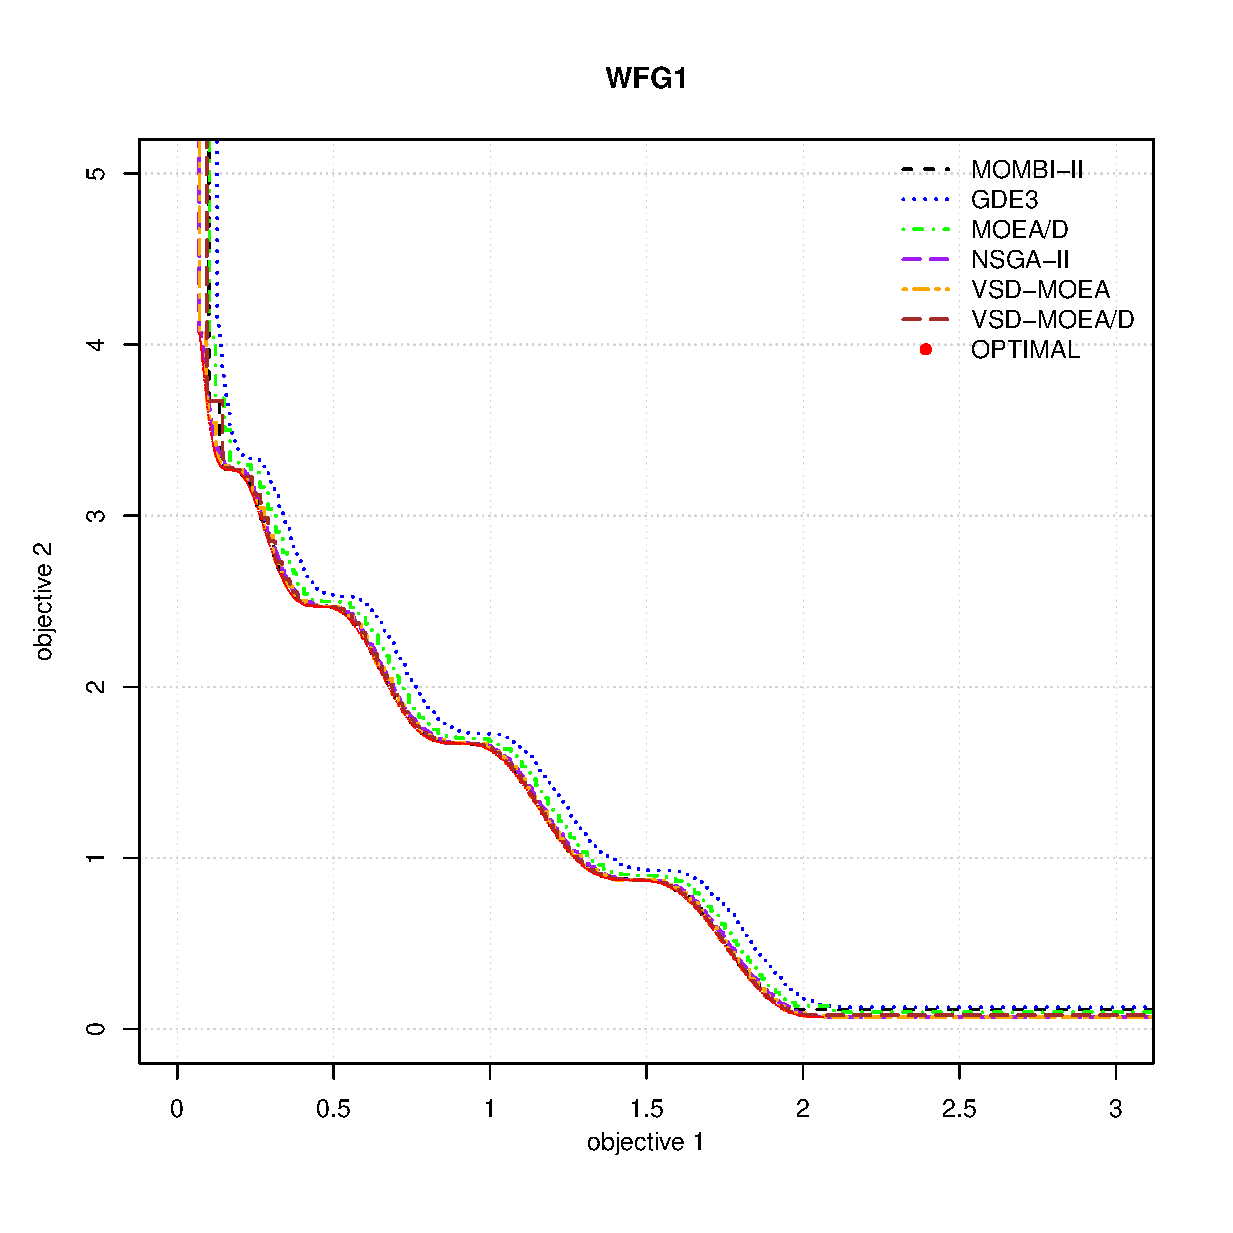
\includegraphics[width=0.33\textwidth]{Figures_Chapter7/Results_Chapter4/Surface_Representative/WFG1.eps}  &
  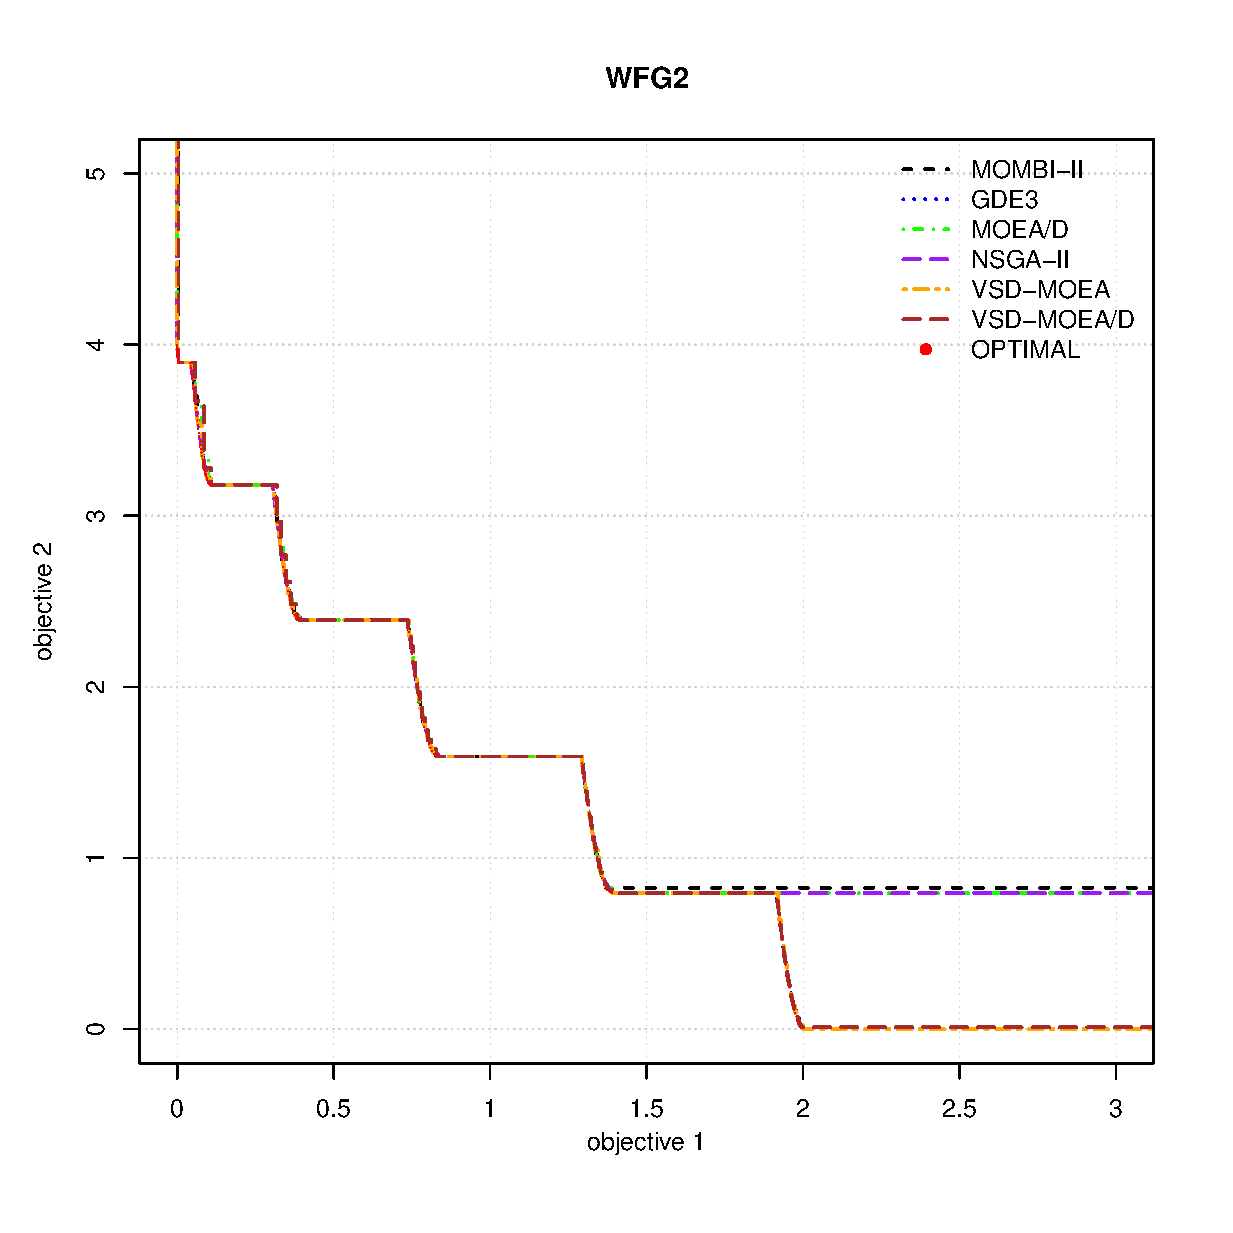
\includegraphics[width=0.33\textwidth]{Figures_Chapter7/Results_Chapter4/Surface_Representative/WFG2.eps} &
  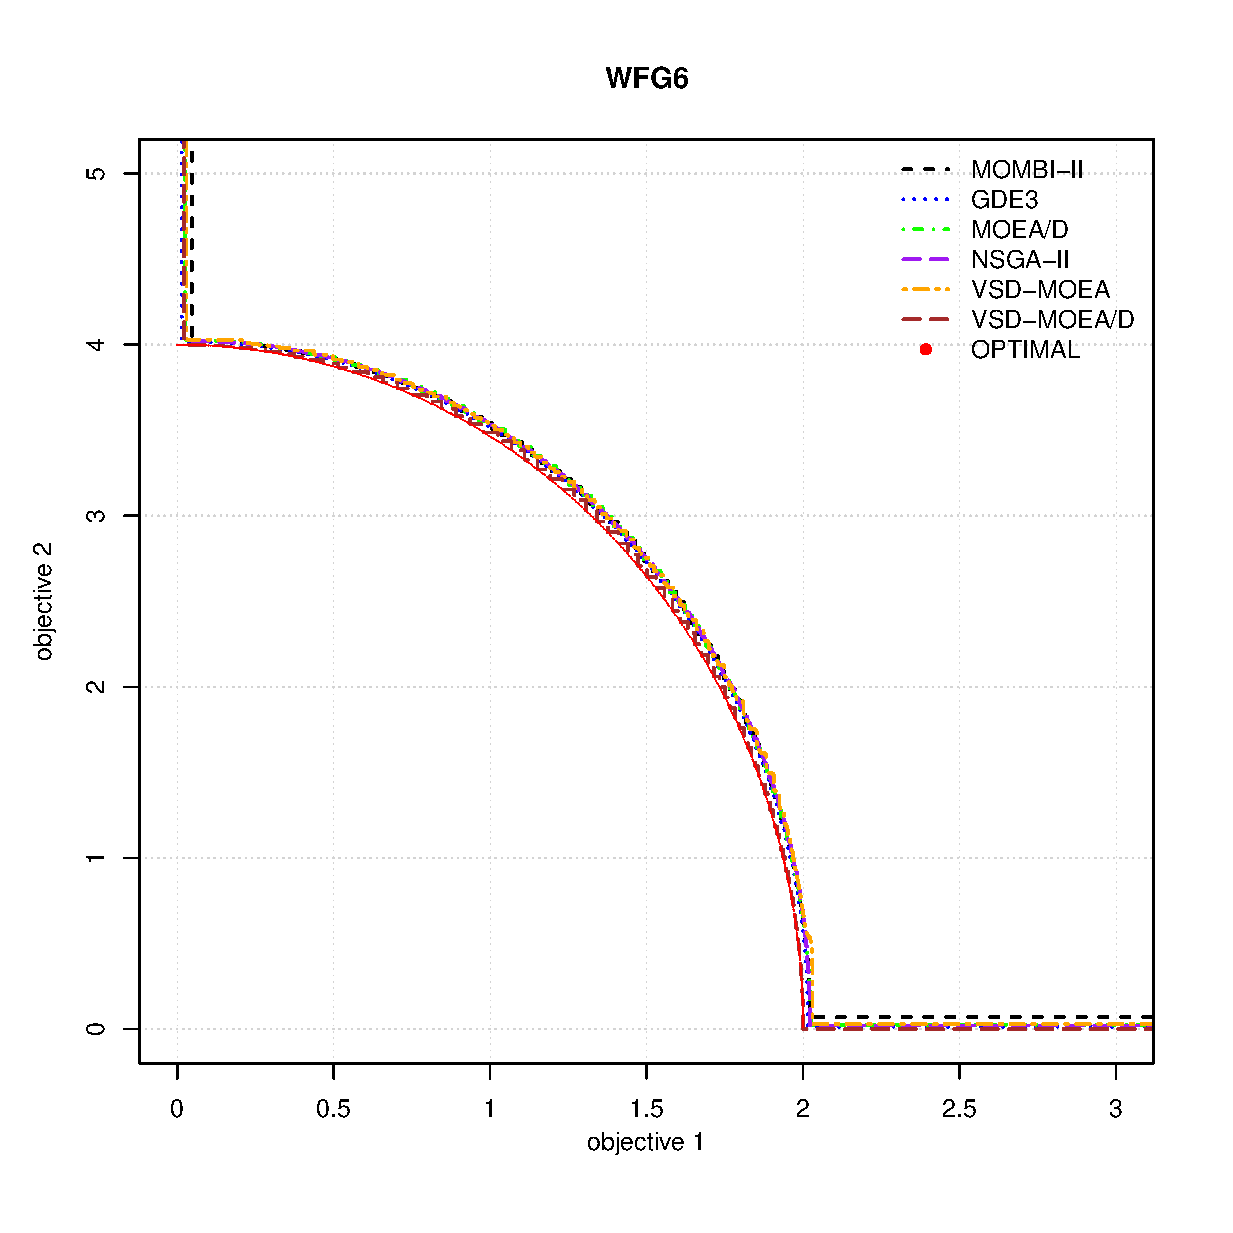
\includegraphics[width=0.33\textwidth]{Figures_Chapter7/Results_Chapter4/Surface_Representative/WFG6.eps} \\
  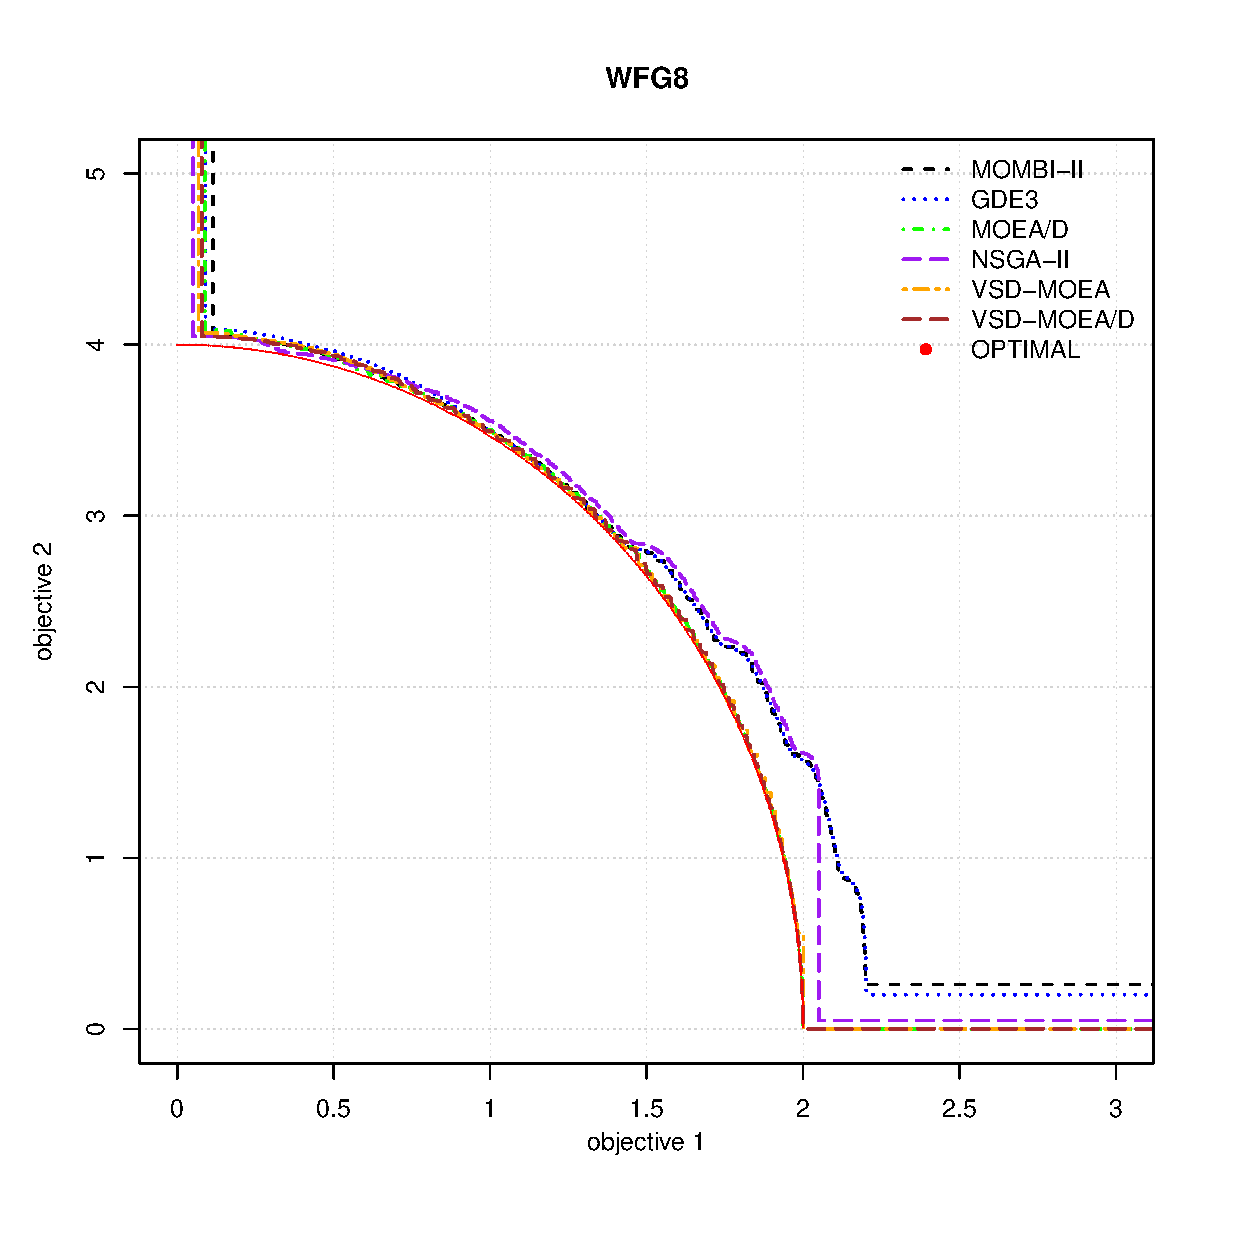
\includegraphics[width=0.33\textwidth]{Figures_Chapter7/Results_Chapter4/Surface_Representative/WFG8.eps} &
  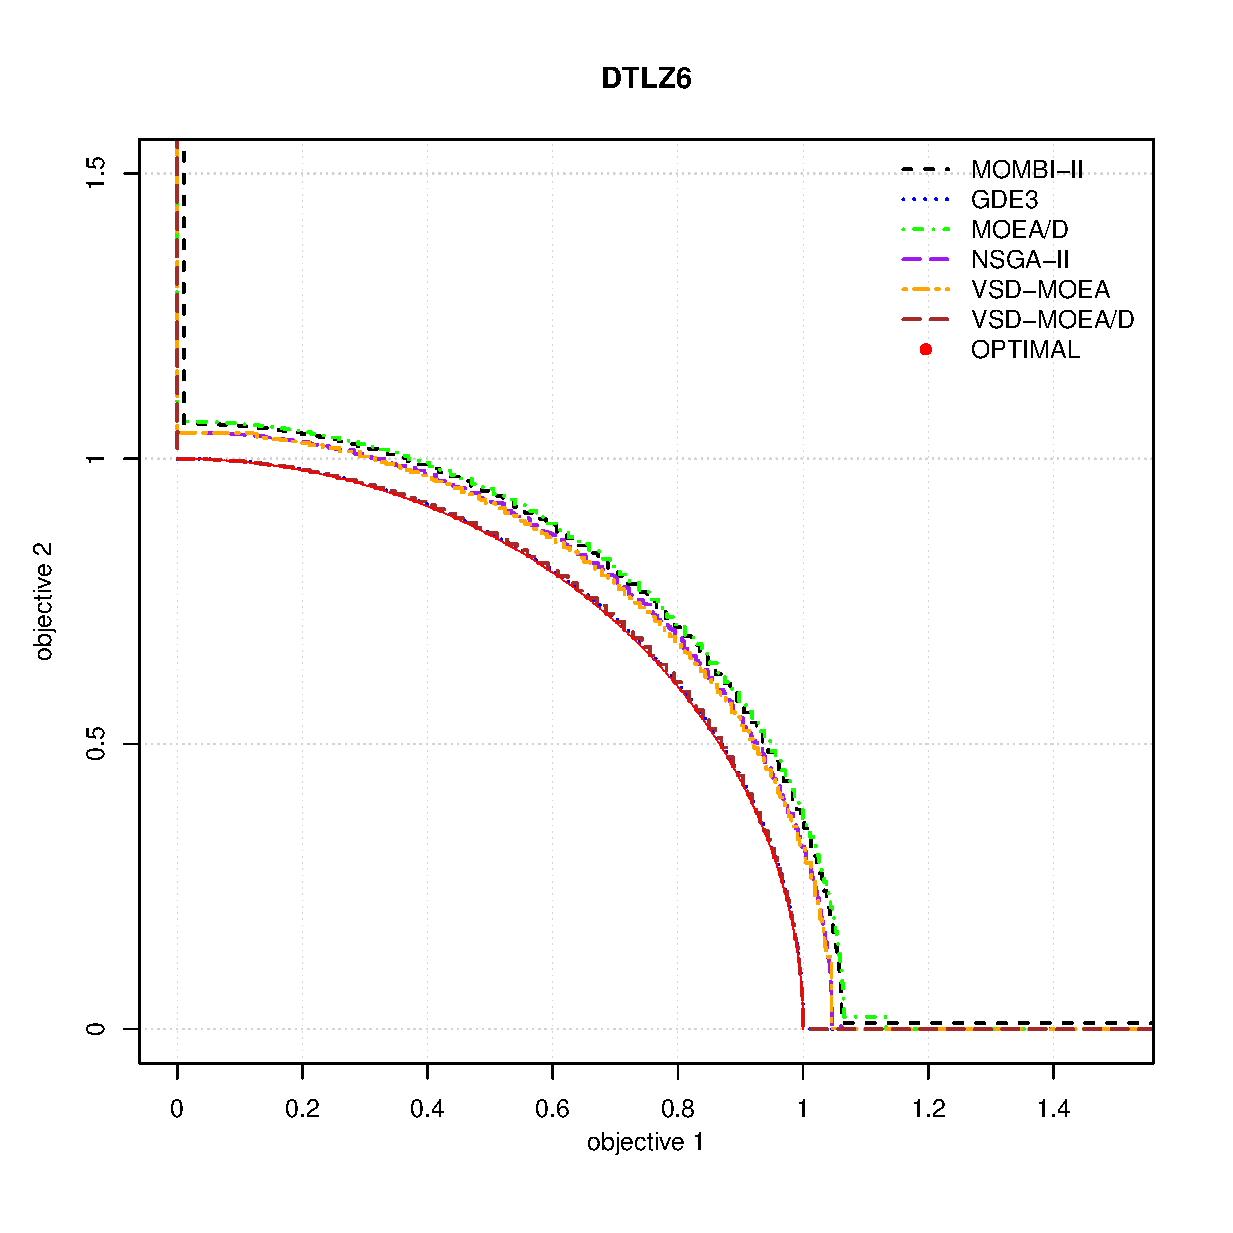
\includegraphics[width=0.33\textwidth]{Figures_Chapter7/Results_Chapter4/Surface_Representative/DTLZ6.eps} &
  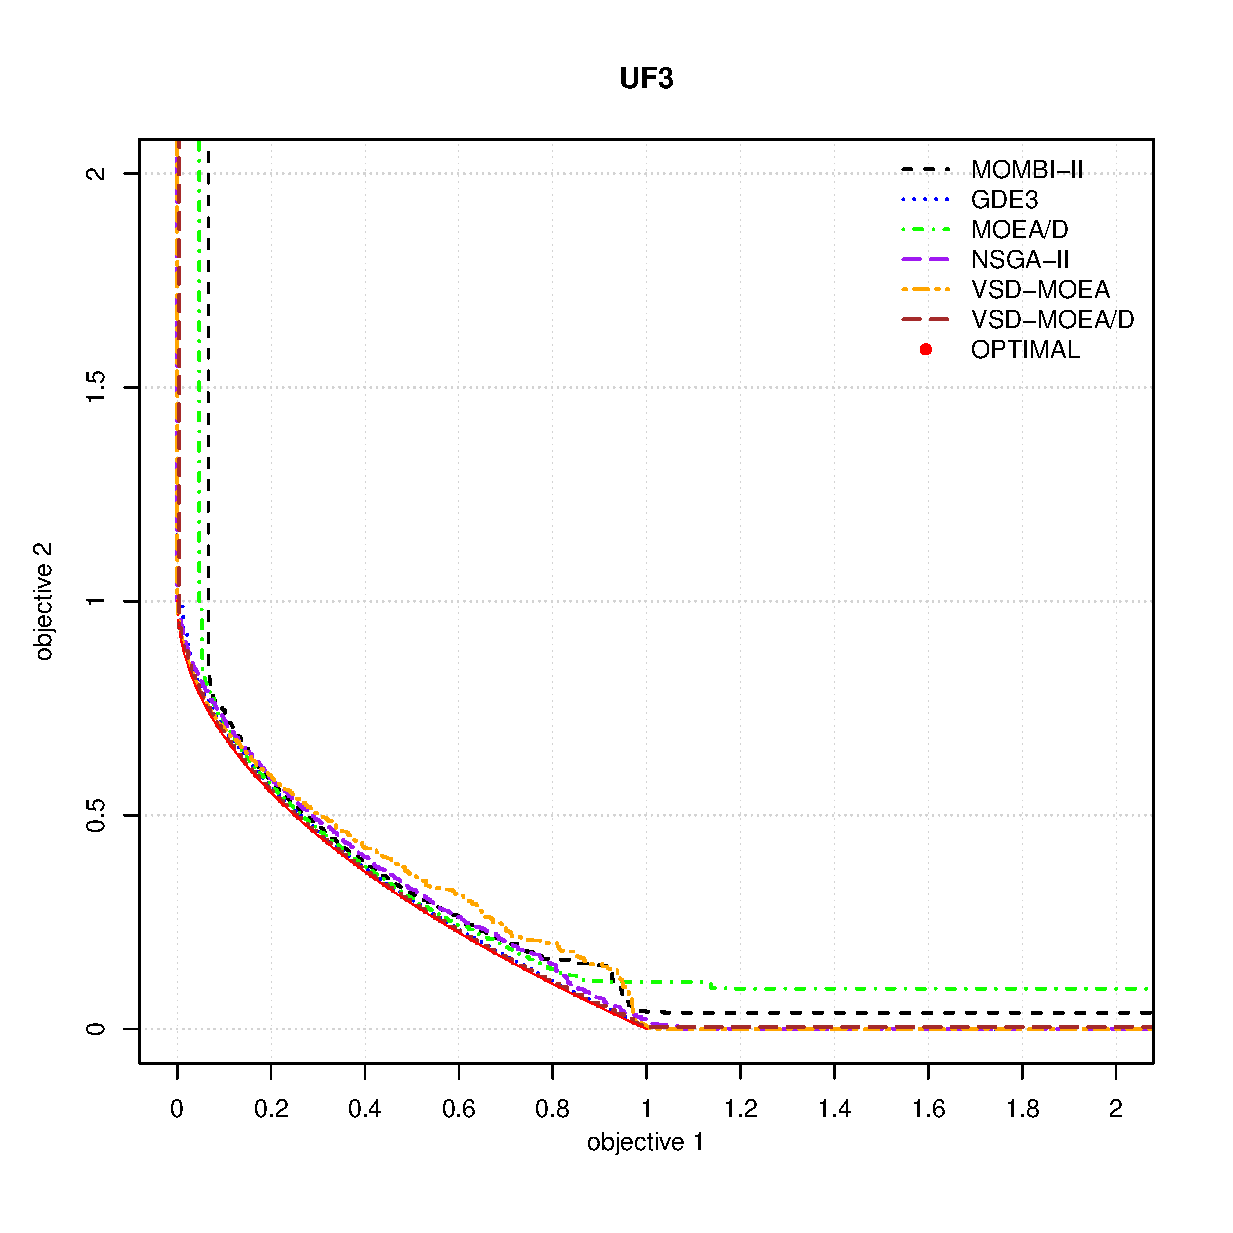
\includegraphics[width=0.33\textwidth]{Figures_Chapter7/Results_Chapter4/Surface_Representative/UF3.eps} \\
  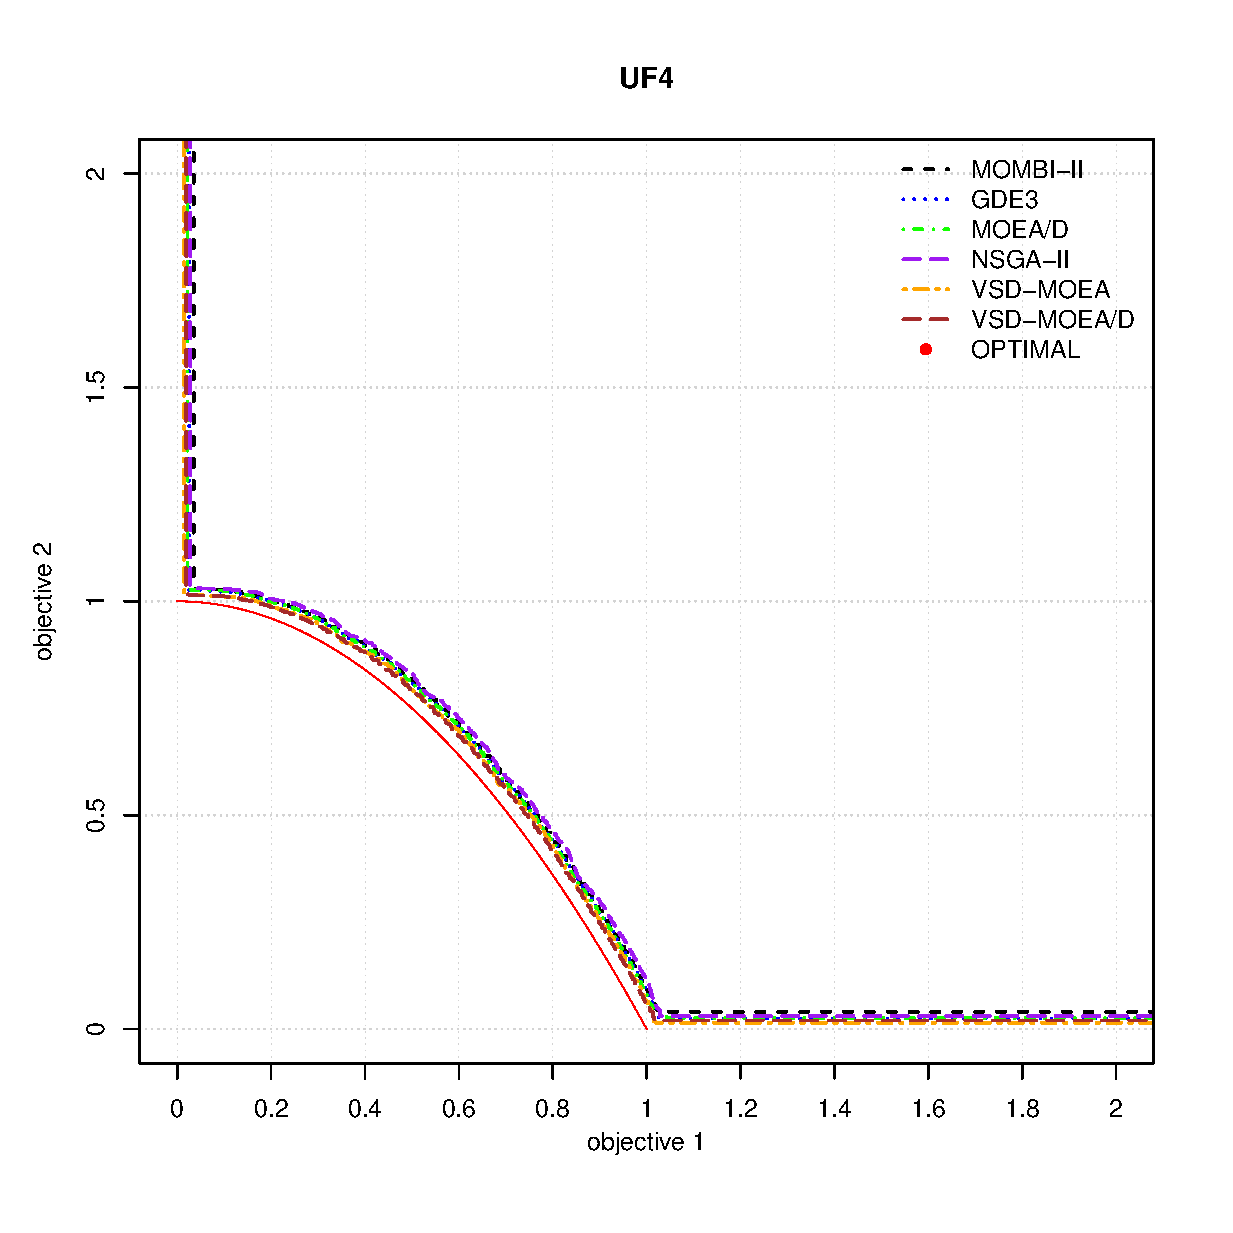
\includegraphics[width=0.33\textwidth]{Figures_Chapter7/Results_Chapter4/Surface_Representative/UF4.eps} &
  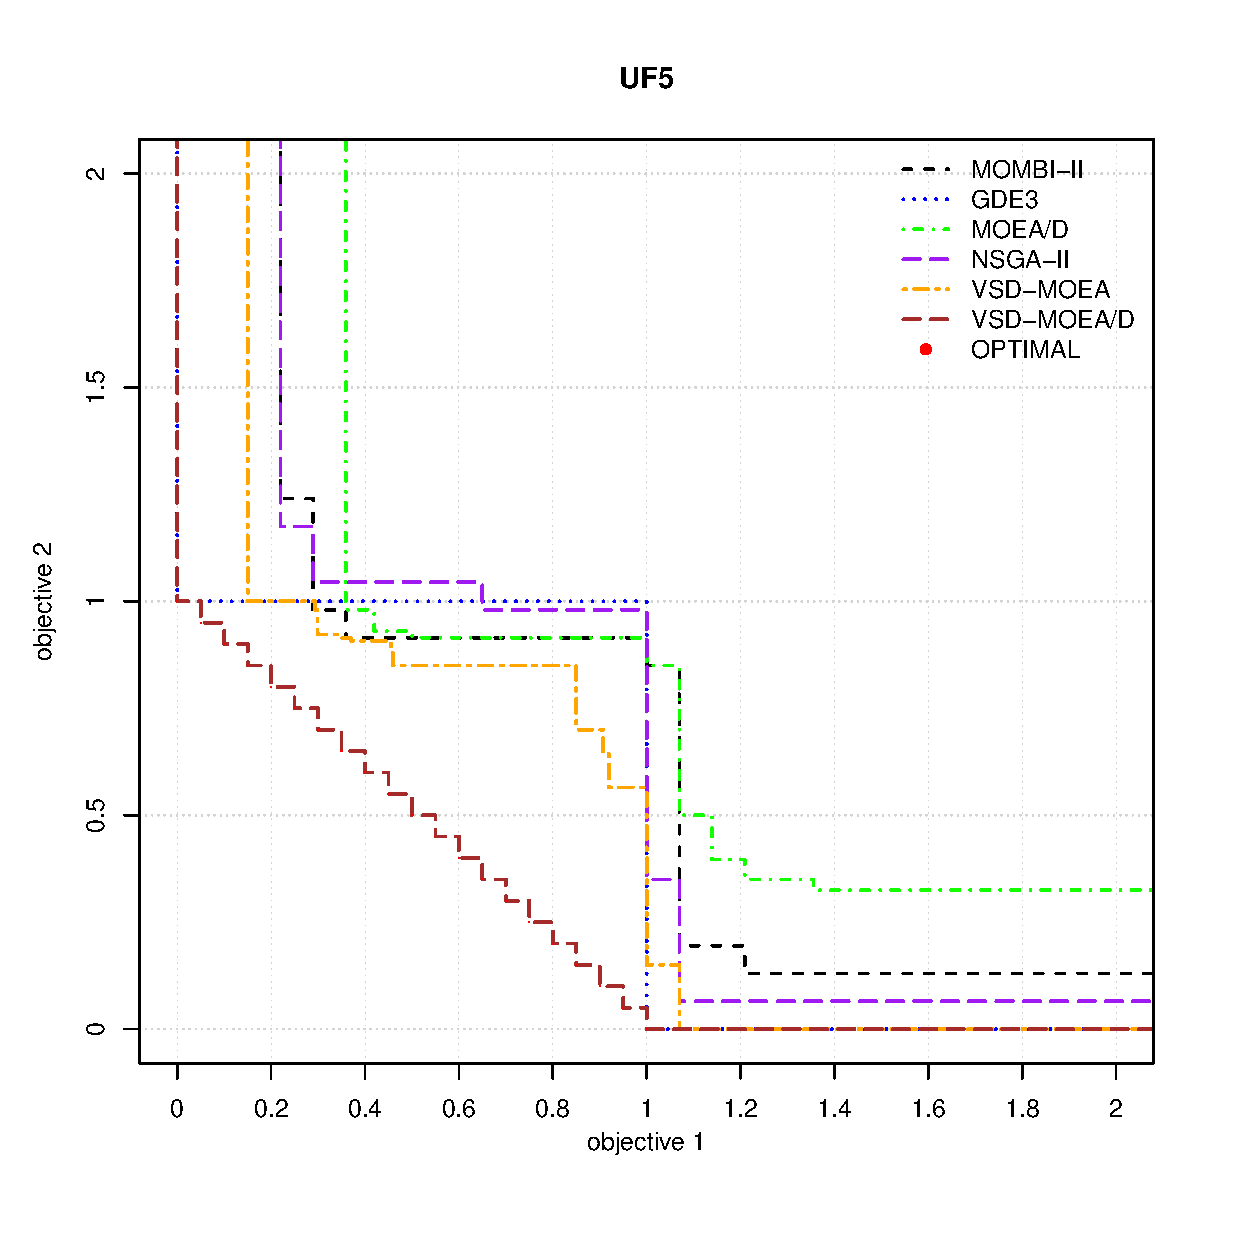
\includegraphics[width=0.33\textwidth]{Figures_Chapter7/Results_Chapter4/Surface_Representative/UF5.eps} &
  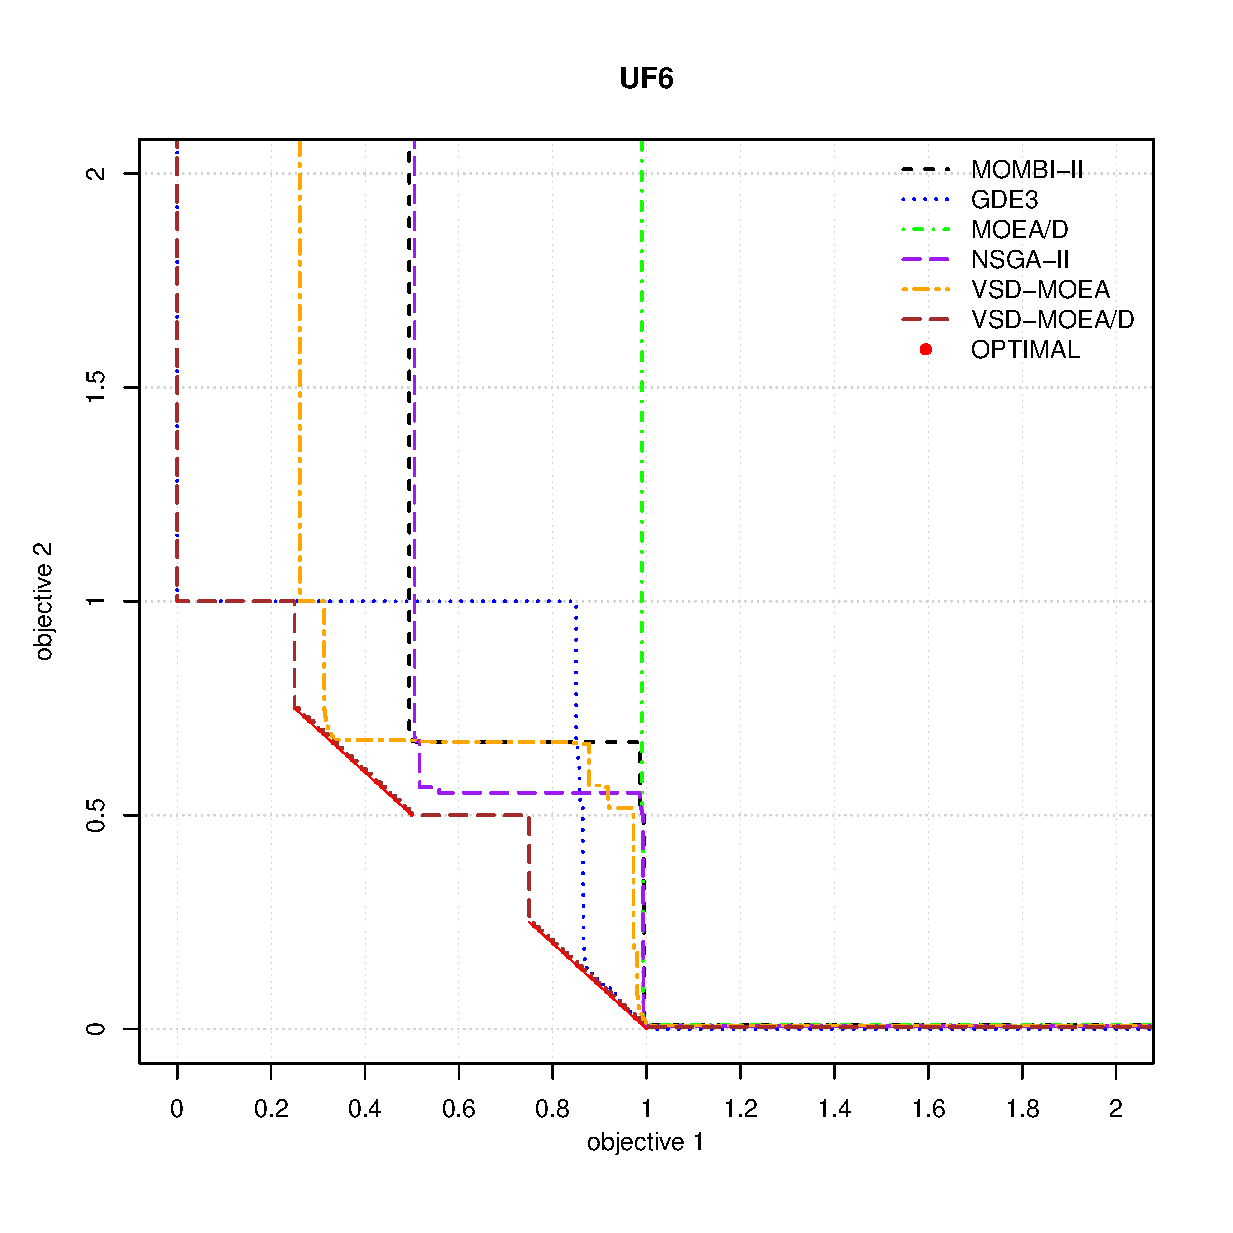
\includegraphics[width=0.33\textwidth]{Figures_Chapter7/Results_Chapter4/Surface_Representative/UF6.eps} 
\end{tabular}
\end{figure}






\section{Operador de cruce SBX}

Esta sección está dedicada para mostrar los experimentos que se realizaron para validar el dendimiento del operador NRD-SBX.
%
Se muestran estudios con los algoritmos NSGA-II, MOEA/D y SMS-EMOA, implementados en el marco de trabajo jMetalcpp (\cite{Joel:jMetal}).
%
El único cambio realizado fue el operador de cruce.
%
La versión de SBX que viene incorporada en jMetalcpp difiere ligeramente a la indicada en la versión oficial del NSGA-II, pues la variante de jMetalcpp incluye un paso de reflexión adicional.
%
En nuestra validación se consideró la versión incluida en el NSGA-II oficial, así como el nuevo operador NRD-SBX.
%
En lo referente a las funciones multi-objetivo, se consideran las 9 funciones WFG. 
%
Se utilizó la configuración indicada al inicio de este capítulo, la única variante es el indice de distribución del operador de mutación, fijado en $20$.
%
Asimismo, el análisis experimental se realizó teniendo en cuenta las superficies de cubrimiento y el hipervolumen.

\begin{figure*}[t] 
\scriptsize
\centering
\begin{tabular}{cccc}
  \multicolumn{2}{c}{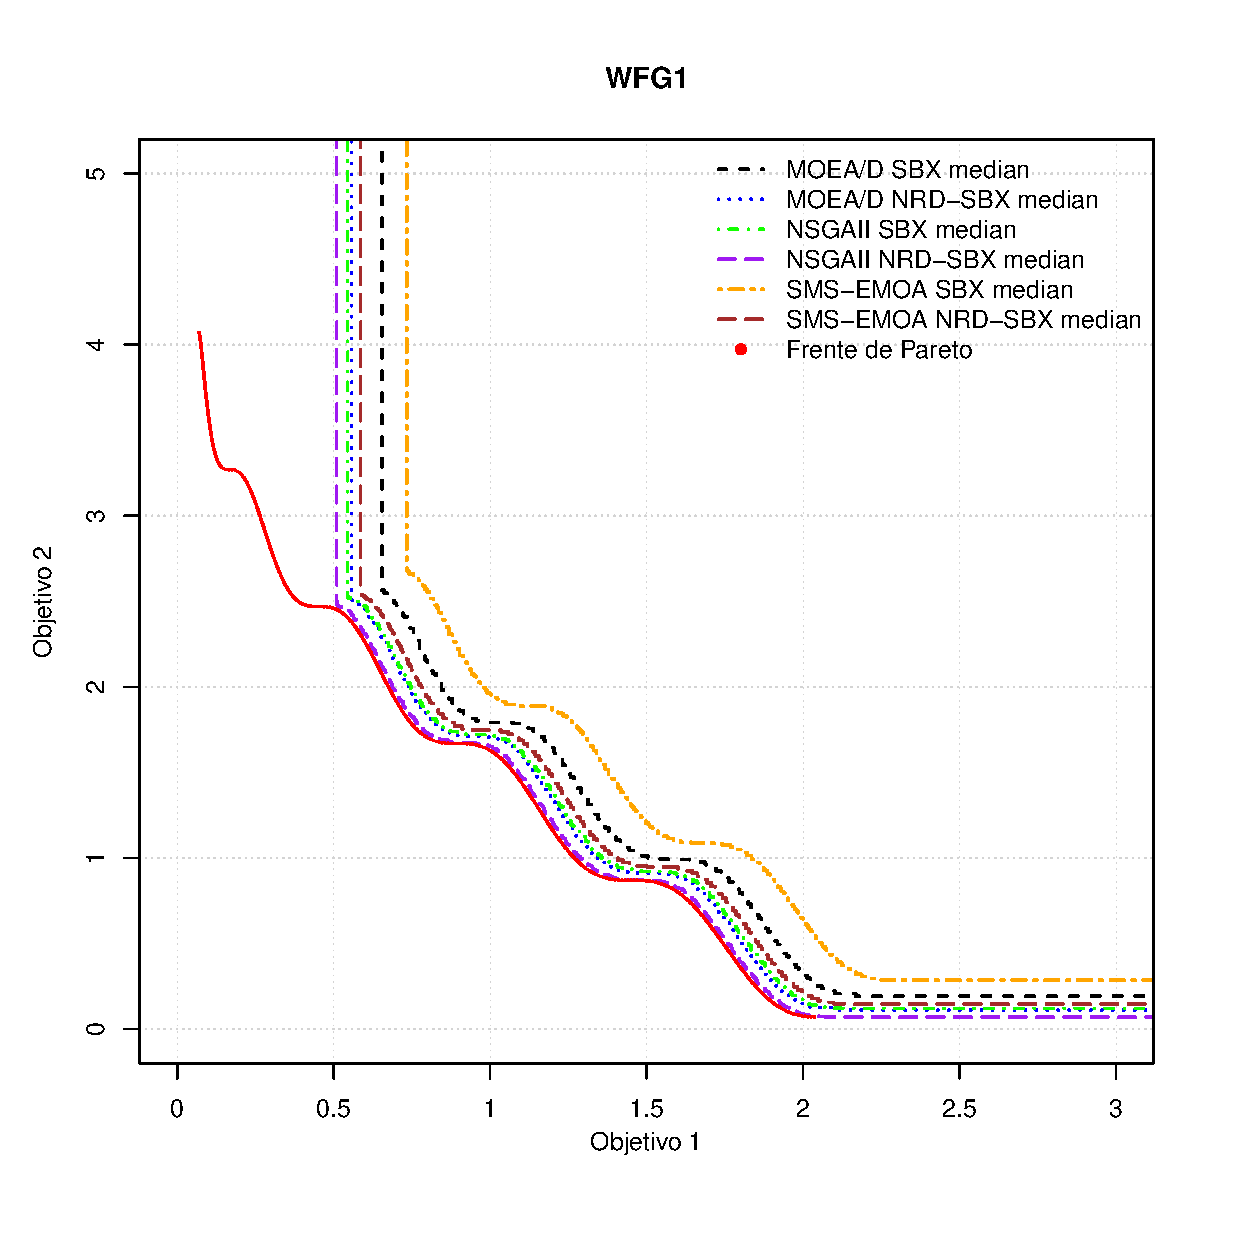
\includegraphics[width=0.40\textwidth]{Figures_Chapter7/Results_Chapter5/WFG1.eps}} &  \multicolumn{2}{c}{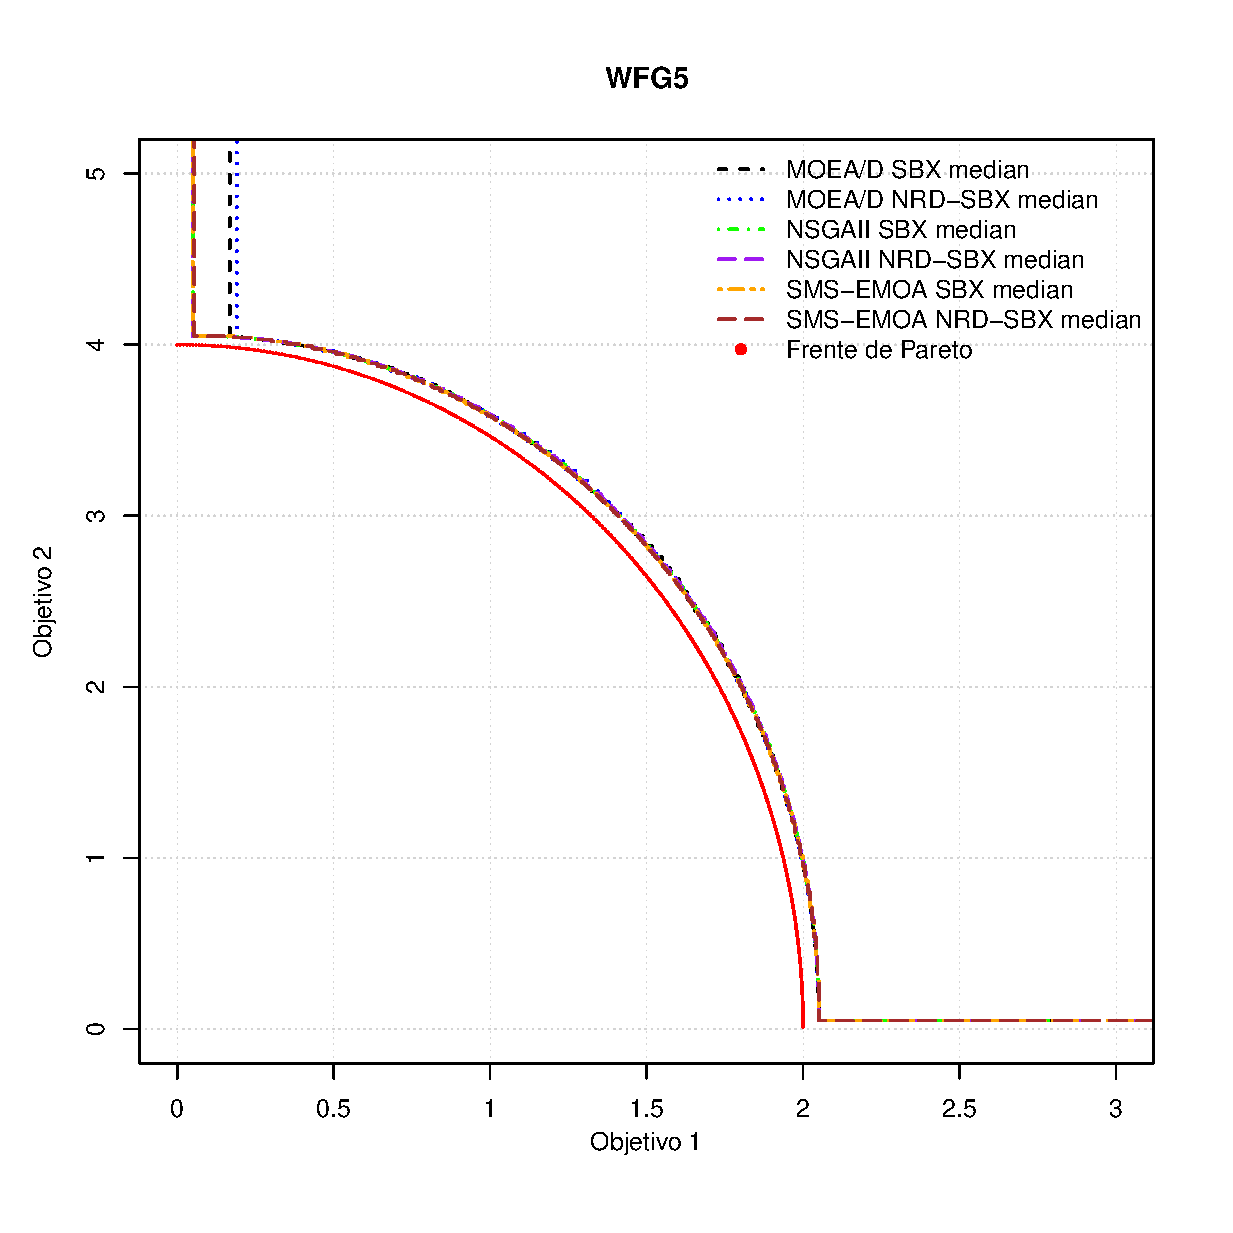
\includegraphics[width=0.40\textwidth]{Figures_Chapter7/Results_Chapter5/WFG5.eps}} \\
  \multicolumn{2}{c}{ \includegraphics[width=0.40\textwidth]{Figures_Chapter7/Results_Chapter5/WFG8.eps}} & \multicolumn{2}{c}{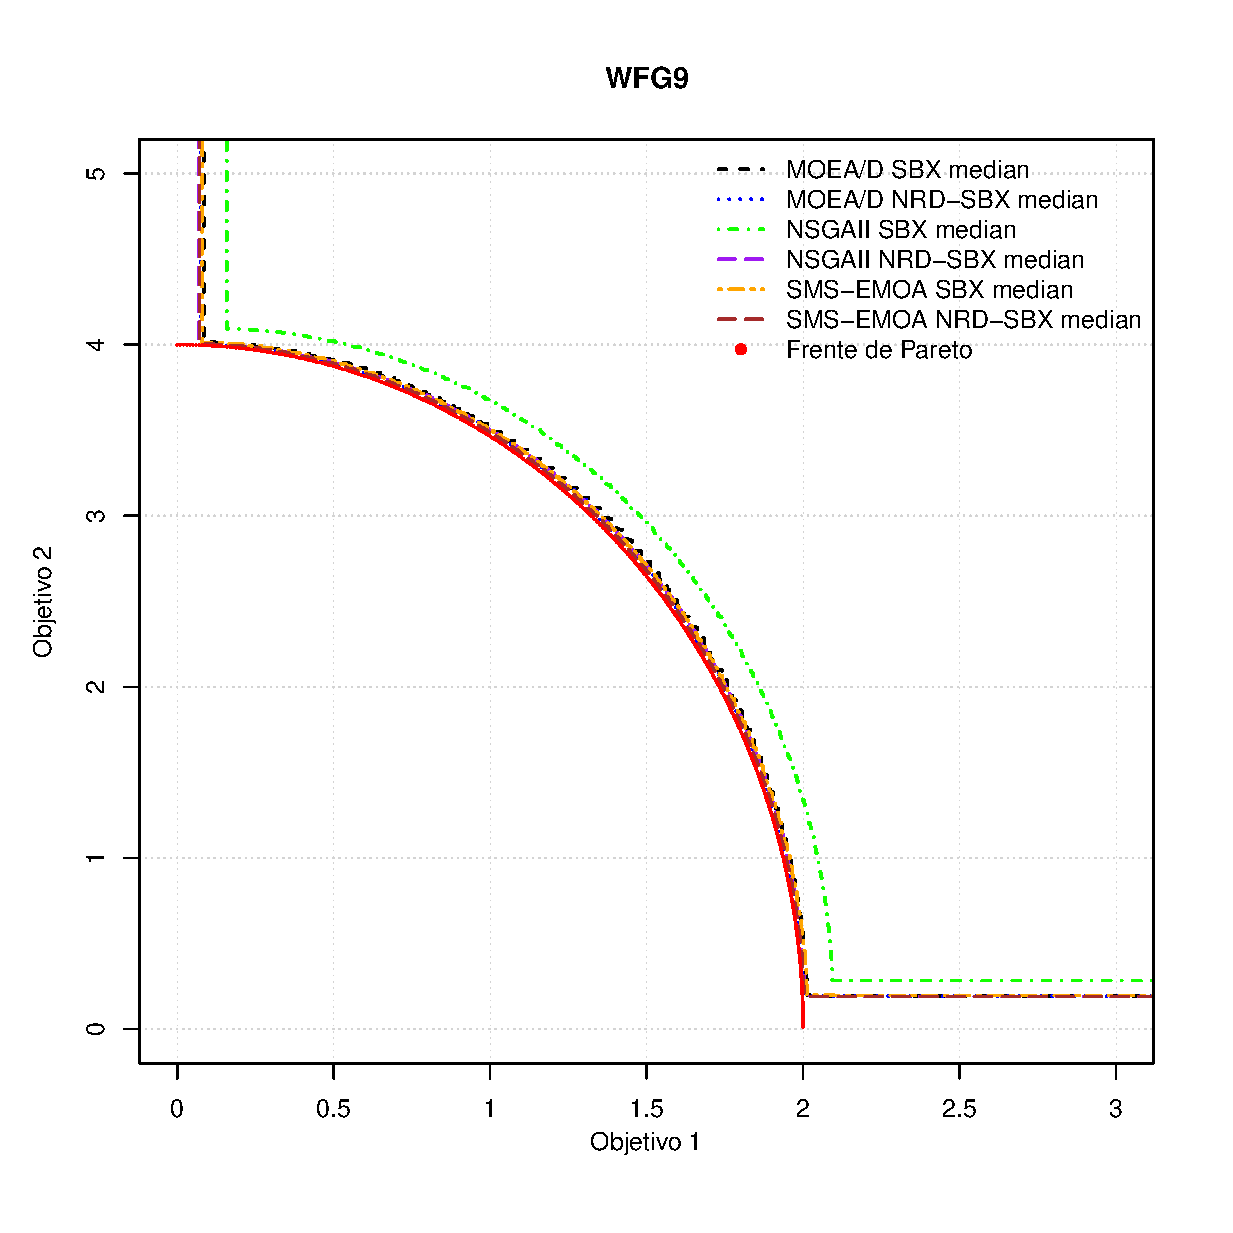
\includegraphics[width=0.40\textwidth]{Figures_Chapter7/Results_Chapter5/WFG9.eps}}
\end{tabular}
\caption{Superficies de cubrimiento al 50\% obtenidas por los diferentes MOEAs con SBX y NRD-SBX}
 \label{fig:Attainment_Surfaces_State_Art_SBX}
\end{figure*}

En primer lugar se van a analizar los resultados en base a las superficies de cubrimiento. 
%
Para ello, de los 9 problemas se seleccionaron los 4 casos en los que se detectaron mayores diferencias, el resto de resultados puede ser consultado en el apéndice \ref{AppendixC}
%
La Figura\ref{fig:Attainment_Surfaces_State_Art_SBX} muestra las superficies de cubrimiento al 50\% del WFG1, WFG5, WFG8 y WFG9.
%
Se puede apreciar que para cada algoritmo, el uso del operador NRD-SBX produce resultados que dominan o igualan a los alcanzados por SBX en la mayor parte de las casos. 
%
De hecho, la única excepción se da en la instancia WFG5 con el NSGA-II, en el que la implementación del NRD-SBX produce resultados ligeramente inferiores.
%
En cualquier caso, los beneficios ofrecidos por el NRD-SBX son superiores que en la penalización de la instancia WFG5.
%
Particularmente, los beneficios de los problemas WFG1 y WFG8 son especialmente claros.
%
En el caso del problema WFG1, se ha mostrado en el capítulo \ref{Chapter1} que la pérdida rápida de la diversidad puede ser un grave problema, con lo que el mayor grado de exploración que induce NRD-SBX en las fases iniciales es de gran ayuda.
%
Por otro lado, dado que es un problema unimodal y separable, evitar las reflexiones y centrarse en crear soluciones cercanas a los padres también contribuye al buen rendimiento.
%
En el caso de la instancia WFG8, hay un alto grado de dependencia entre las variables, por lo tanto cambiar de forma dinámica el grado de similitud de los individuos creados es de gran ayuda.
%
En el problema WFG9 se da una situación similar, aunque por ser más sencilla, los beneficios sólo se aprecian de forma clara en el caso del NSGA-II.

\begin{table}[t]
\begin{center}
\begin{scriptsize}
\centering
\caption{Valores de hipervolumen alcanzados por los diferentes MOEAs con los operadores de cruce SBX y NRD-SBX}
\label{tab:Estadisticas_HV}
\begin{tabular}{ccccccccc}
                           & \multicolumn{8}{c}{MOEA/D}                                                                                                                                                                                                                                                                                     \\ \cline{2-9} 
\multicolumn{1}{c|}{}      & \multicolumn{4}{c|}{NRD-SBX}                                                                                                                             & \multicolumn{4}{c|}{SBX}                                                                                                                             \\ \hline
\multicolumn{1}{|c|}{}     & \multicolumn{1}{c|}{Min.}            & \multicolumn{1}{c|}{Max.}            & \multicolumn{1}{c|}{Media}           & \multicolumn{1}{c|}{Desv.}               & \multicolumn{1}{c|}{Min.}           & \multicolumn{1}{c|}{Max.}           & \multicolumn{1}{c|}{Media}          & \multicolumn{1}{c|}{Desv.}               \\ \hline
\multicolumn{1}{|c|}{WFG1} & \multicolumn{1}{c|}{\textbf{9.61}}  & \multicolumn{1}{c|}{\textbf{10.72}} & \multicolumn{1}{c|}{\textbf{10.26}} & \multicolumn{1}{c|}{\textbf{3.1E-01}} & \multicolumn{1}{c|}{8.39}          & \multicolumn{1}{c|}{10.29}         & \multicolumn{1}{c|}{9.62}          & \multicolumn{1}{c|}{4.3E-01}          \\ \hline
\multicolumn{1}{|c|}{WFG2} & \multicolumn{1}{c|}{\textbf{10.62}} & \multicolumn{1}{c|}{\textbf{11.45}} & \multicolumn{1}{c|}{\textbf{10.66}} & \multicolumn{1}{c|}{\textbf{1.9E-01}} & \multicolumn{1}{c|}{9.28}          & \multicolumn{1}{c|}{10.62}         & \multicolumn{1}{c|}{10.50}         & \multicolumn{1}{c|}{3.7E-01}          \\ \hline
\multicolumn{1}{|c|}{WFG3} & \multicolumn{1}{c|}{10.95}          & \multicolumn{1}{c|}{10.95}          & \multicolumn{1}{c|}{10.95}          & \multicolumn{1}{c|}{2.5E-04}          & \multicolumn{1}{c|}{10.95}         & \multicolumn{1}{c|}{10.95}         & \multicolumn{1}{c|}{10.95}         & \multicolumn{1}{c|}{3.0E-04}          \\ \hline
\multicolumn{1}{|c|}{WFG4} & \multicolumn{1}{c|}{8.68}           & \multicolumn{1}{c|}{8.68}           & \multicolumn{1}{c|}{8.68}           & \multicolumn{1}{c|}{1.0E-04}          & \multicolumn{1}{c|}{8.67}          & \multicolumn{1}{c|}{8.68}          & \multicolumn{1}{c|}{8.68}          & \multicolumn{1}{c|}{1.0E-04}          \\ \hline
\multicolumn{1}{|c|}{WFG5} & \multicolumn{1}{c|}{8.13}           & \multicolumn{1}{c|}{8.34}           & \multicolumn{1}{c|}{8.16}           & \multicolumn{1}{c|}{4.7E-02}          & \multicolumn{1}{c|}{\textbf{8.13}} & \multicolumn{1}{c|}{\textbf{8.24}} & \multicolumn{1}{c|}{\textbf{8.19}} & \multicolumn{1}{c|}{\textbf{3.0E-02}} \\ \hline
\multicolumn{1}{|c|}{WFG6} & \multicolumn{1}{c|}{\textbf{8.39}}  & \multicolumn{1}{c|}{\textbf{8.57}}  & \multicolumn{1}{c|}{\textbf{8.49}}  & \multicolumn{1}{c|}{\textbf{4.8E-02}} & \multicolumn{1}{c|}{7.76}          & \multicolumn{1}{c|}{8.54}          & \multicolumn{1}{c|}{8.30}          & \multicolumn{1}{c|}{1.2E-01}          \\ \hline
\multicolumn{1}{|c|}{WFG7} & \multicolumn{1}{c|}{8.67}           & \multicolumn{1}{c|}{8.68}           & \multicolumn{1}{c|}{8.67}           & \multicolumn{1}{c|}{1.5E-04}          & \multicolumn{1}{c|}{8.67}          & \multicolumn{1}{c|}{8.68}          & \multicolumn{1}{c|}{8.67}          & \multicolumn{1}{c|}{2.3E-04}          \\ \hline
\multicolumn{1}{|c|}{WFG8} & \multicolumn{1}{c|}{\textbf{8.20}}  & \multicolumn{1}{c|}{\textbf{8.60}}  & \multicolumn{1}{c|}{\textbf{8.54}}  & \multicolumn{1}{c|}{\textbf{8.5E-02}} & \multicolumn{1}{c|}{7.80}          & \multicolumn{1}{c|}{7.87}          & \multicolumn{1}{c|}{7.83}          & \multicolumn{1}{c|}{1.8E-02}          \\ \hline
\multicolumn{1}{|c|}{WFG9} & \multicolumn{1}{c|}{\textbf{7.70}}  & \multicolumn{1}{c|}{\textbf{8.56}}  & \multicolumn{1}{c|}{\textbf{8.41}}  & \multicolumn{1}{c|}{\textbf{1.9E-01}} & \multicolumn{1}{c|}{7.70}          & \multicolumn{1}{c|}{8.54}          & \multicolumn{1}{c|}{8.20}          & \multicolumn{1}{c|}{3.1E-01}          \\ \hline
% \end{tabular}
% \end{table}


% \begin{table}[]
% \centering
% \caption{My caption}
% \label{my-label}
% \begin{tabular}{ccccccccc}
                           & \multicolumn{8}{c}{NSGA-II}                                                                                                                                                                                                                                                                                       \\ \cline{2-9} 
\multicolumn{1}{c|}{}      & \multicolumn{4}{c|}{NRD-SBX}                                                                                                                             & \multicolumn{4}{c|}{SBX}                                                                                                                                \\ \hline
\multicolumn{1}{|c|}{}     & \multicolumn{1}{c|}{Min.}            & \multicolumn{1}{c|}{Max.}            & \multicolumn{1}{c|}{Media}           & \multicolumn{1}{c|}{Desv.}               & \multicolumn{1}{c|}{Min.}            & \multicolumn{1}{c|}{Max.}            & \multicolumn{1}{c|}{Media}           & \multicolumn{1}{c|}{Desv.}               \\ \hline
\multicolumn{1}{|c|}{WFG1} & \multicolumn{1}{c|}{\textbf{9.91}}  & \multicolumn{1}{c|}{\textbf{10.70}} & \multicolumn{1}{c|}{\textbf{10.52}} & \multicolumn{1}{c|}{\textbf{1.8E-01}} & \multicolumn{1}{c|}{9.51}           & \multicolumn{1}{c|}{10.76}          & \multicolumn{1}{c|}{10.21}          & \multicolumn{1}{c|}{3.1E-01}          \\ \hline
\multicolumn{1}{|c|}{WFG2} & \multicolumn{1}{c|}{\textbf{10.59}} & \multicolumn{1}{c|}{\textbf{11.44}} & \multicolumn{1}{c|}{\textbf{10.66}} & \multicolumn{1}{c|}{\textbf{1.9E-01}} & \multicolumn{1}{c|}{9.28}           & \multicolumn{1}{c|}{10.62}          & \multicolumn{1}{c|}{10.58}          & \multicolumn{1}{c|}{2.2E-01}          \\ \hline
\multicolumn{1}{|c|}{WFG3} & \multicolumn{1}{c|}{10.91}          & \multicolumn{1}{c|}{10.93}          & \multicolumn{1}{c|}{10.92}          & \multicolumn{1}{c|}{4.0E-03}          & \multicolumn{1}{c|}{\textbf{10.92}} & \multicolumn{1}{c|}{\textbf{10.93}} & \multicolumn{1}{c|}{\textbf{10.93}} & \multicolumn{1}{c|}{\textbf{2.7E-03}} \\ \hline
\multicolumn{1}{|c|}{WFG4} & \multicolumn{1}{c|}{8.65}           & \multicolumn{1}{c|}{8.66}           & \multicolumn{1}{c|}{8.66}           & \multicolumn{1}{c|}{2.3E-03}          & \multicolumn{1}{c|}{\textbf{8.66}}  & \multicolumn{1}{c|}{\textbf{8.67}}  & \multicolumn{1}{c|}{\textbf{8.67}}  & \multicolumn{1}{c|}{\textbf{2.2E-03}} \\ \hline
\multicolumn{1}{|c|}{WFG5} & \multicolumn{1}{c|}{8.26}           & \multicolumn{1}{c|}{8.27}           & \multicolumn{1}{c|}{8.27}           & \multicolumn{1}{c|}{2.3E-03}          & \multicolumn{1}{c|}{8.27}           & \multicolumn{1}{c|}{8.28}           & \multicolumn{1}{c|}{8.27}           & \multicolumn{1}{c|}{1.6E-03}          \\ \hline
\multicolumn{1}{|c|}{WFG6} & \multicolumn{1}{c|}{\textbf{8.33}}  & \multicolumn{1}{c|}{\textbf{8.59}}  & \multicolumn{1}{c|}{\textbf{8.47}}  & \multicolumn{1}{c|}{\textbf{5.6E-02}} & \multicolumn{1}{c|}{8.12}           & \multicolumn{1}{c|}{8.46}           & \multicolumn{1}{c|}{8.34}           & \multicolumn{1}{c|}{6.5E-02}          \\ \hline
\multicolumn{1}{|c|}{WFG7} & \multicolumn{1}{c|}{8.64}           & \multicolumn{1}{c|}{8.66}           & \multicolumn{1}{c|}{8.65}           & \multicolumn{1}{c|}{3.9E-03}          & \multicolumn{1}{c|}{\textbf{8.66}}  & \multicolumn{1}{c|}{\textbf{8.67}}  & \multicolumn{1}{c|}{\textbf{8.66}}  & \multicolumn{1}{c|}{\textbf{2.6E-03}} \\ \hline
\multicolumn{1}{|c|}{WFG8} & \multicolumn{1}{c|}{\textbf{7.88}}  & \multicolumn{1}{c|}{\textbf{8.50}}  & \multicolumn{1}{c|}{\textbf{8.26}}  & \multicolumn{1}{c|}{\textbf{2.7E-01}} & \multicolumn{1}{c|}{7.71}           & \multicolumn{1}{c|}{7.83}           & \multicolumn{1}{c|}{7.78}           & \multicolumn{1}{c|}{3.2E-02}          \\ \hline
\multicolumn{1}{|c|}{WFG9} & \multicolumn{1}{c|}{\textbf{8.34}}  & \multicolumn{1}{c|}{\textbf{8.61}}  & \multicolumn{1}{c|}{\textbf{8.43}}  & \multicolumn{1}{c|}{\textbf{7.9E-02}} & \multicolumn{1}{c|}{7.69}           & \multicolumn{1}{c|}{8.51}           & \multicolumn{1}{c|}{7.85}           & \multicolumn{1}{c|}{2.8E-01}          \\ \hline
% \end{tabular}
% \end{table}

% \begin{table}[]
% \centering
% \caption{My caption}
% \label{my-label}
% \begin{tabular}{ccccccccc}
                           & \multicolumn{8}{c}{SMS-EMOA}                                                                                                                                                                                                                                                                                   \\ \cline{2-9} 
\multicolumn{1}{c|}{}      & \multicolumn{4}{c|}{NRD-SBX}                                                                                                                             & \multicolumn{4}{c|}{SBX}                                                                                                                             \\ \hline
\multicolumn{1}{|c|}{}     & \multicolumn{1}{c|}{Min.}            & \multicolumn{1}{c|}{Max.}            & \multicolumn{1}{c|}{Media}           & \multicolumn{1}{c|}{Desv.}               & \multicolumn{1}{c|}{Min.}           & \multicolumn{1}{c|}{Max.}           & \multicolumn{1}{c|}{Media}          & \multicolumn{1}{c|}{Desv.}               \\ \hline
\multicolumn{1}{|c|}{WFG1} & \multicolumn{1}{c|}{\textbf{8.60}}  & \multicolumn{1}{c|}{\textbf{10.70}} & \multicolumn{1}{c|}{\textbf{10.03}} & \multicolumn{1}{c|}{\textbf{4.6E-01}} & \multicolumn{1}{c|}{8.00}          & \multicolumn{1}{c|}{9.89}          & \multicolumn{1}{c|}{8.92}          & \multicolumn{1}{c|}{5.0E-01}          \\ \hline
\multicolumn{1}{|c|}{WFG2} & \multicolumn{1}{c|}{\textbf{10.63}} & \multicolumn{1}{c|}{\textbf{11.46}} & \multicolumn{1}{c|}{\textbf{10.65}} & \multicolumn{1}{c|}{\textbf{1.4E-01}} & \multicolumn{1}{c|}{9.29}          & \multicolumn{1}{c|}{11.46}         & \multicolumn{1}{c|}{10.61}         & \multicolumn{1}{c|}{2.7E-01}          \\ \hline
\multicolumn{1}{|c|}{WFG3} & \multicolumn{1}{c|}{10.96}          & \multicolumn{1}{c|}{10.96}          & \multicolumn{1}{c|}{10.96}          & \multicolumn{1}{c|}{2.8E-04}          & \multicolumn{1}{c|}{10.96}         & \multicolumn{1}{c|}{10.96}         & \multicolumn{1}{c|}{10.96}         & \multicolumn{1}{c|}{3.6E-04}          \\ \hline
\multicolumn{1}{|c|}{WFG4} & \multicolumn{1}{c|}{8.69}           & \multicolumn{1}{c|}{8.69}           & \multicolumn{1}{c|}{8.69}           & \multicolumn{1}{c|}{7.7E-06}          & \multicolumn{1}{c|}{8.69}          & \multicolumn{1}{c|}{8.69}          & \multicolumn{1}{c|}{8.69}          & \multicolumn{1}{c|}{6.8E-06}          \\ \hline
\multicolumn{1}{|c|}{WFG5} & \multicolumn{1}{c|}{8.22}           & \multicolumn{1}{c|}{8.29}           & \multicolumn{1}{c|}{8.27}           & \multicolumn{1}{c|}{2.1E-02}          & \multicolumn{1}{c|}{\textbf{8.25}} & \multicolumn{1}{c|}{\textbf{8.29}} & \multicolumn{1}{c|}{\textbf{8.29}} & \multicolumn{1}{c|}{\textbf{8.6E-03}} \\ \hline
\multicolumn{1}{|c|}{WFG6} & \multicolumn{1}{c|}{\textbf{8.36}}  & \multicolumn{1}{c|}{\textbf{8.58}}  & \multicolumn{1}{c|}{\textbf{8.50}}  & \multicolumn{1}{c|}{\textbf{4.7E-02}} & \multicolumn{1}{c|}{8.22}          & \multicolumn{1}{c|}{8.47}          & \multicolumn{1}{c|}{8.34}          & \multicolumn{1}{c|}{5.8E-02}          \\ \hline
\multicolumn{1}{|c|}{WFG7} & \multicolumn{1}{c|}{8.69}           & \multicolumn{1}{c|}{8.69}           & \multicolumn{1}{c|}{8.69}           & \multicolumn{1}{c|}{4.6E-06}          & \multicolumn{1}{c|}{8.69}          & \multicolumn{1}{c|}{8.69}          & \multicolumn{1}{c|}{8.69}          & \multicolumn{1}{c|}{6.5E-06}          \\ \hline
\multicolumn{1}{|c|}{WFG8} & \multicolumn{1}{c|}{\textbf{7.98}}  & \multicolumn{1}{c|}{\textbf{8.61}}  & \multicolumn{1}{c|}{\textbf{8.12}}  & \multicolumn{1}{c|}{\textbf{2.2E-01}} & \multicolumn{1}{c|}{7.81}          & \multicolumn{1}{c|}{7.89}          & \multicolumn{1}{c|}{7.85}          & \multicolumn{1}{c|}{2.2E-02}          \\ \hline
\multicolumn{1}{|c|}{WFG9} & \multicolumn{1}{c|}{\textbf{8.33}}  & \multicolumn{1}{c|}{\textbf{8.66}}  & \multicolumn{1}{c|}{\textbf{8.47}}  & \multicolumn{1}{c|}{\textbf{8.7E-02}} & \multicolumn{1}{c|}{7.71}          & \multicolumn{1}{c|}{8.56}          & \multicolumn{1}{c|}{8.20}          & \multicolumn{1}{c|}{3.1E-01}          \\ \hline
\end{tabular}
\end{scriptsize}
\end{center}
\end{table}


Con el objetivo de confirmar y complementar los hallazgos anteriores, se realiza el análisis del hipervolumen alcanzado por los diferentes algoritmos, con cada uno de los operadores de cruce.
%
La Tabla~\ref{tab:Estadisticas_HV} muestra para cada algoritmo y operador de cruce el mínimo, máximo, media y desviación estándar de los valores del hipervolumen alcanzados.
%
Para el cálculo del hipervolumen se fijó el punto de referencia en (3.0, 5.0) como es indicado en \cite{Joel:OperatorAHX}.
%
Para cada algoritmo y problema, se realizaron comparativas estadísticas entre el operador SBX y el operador NRD-SBX.
%
En los casos en los que se pudo confirmar la superioridad de alguno de los operadores, se resaltan los datos en la tabla.
%
Para el caso del MOEA/D la superioridad del NRD-SBX se pudo confirmar en cinco instancias, mientras que sólo fue inferior en uno; en el NSGA-II, NRD-SBX fue superior en 5 casos e inferior en 3; finalmente en el SMS-EMOA, NRD-SBX fue superior en 5 casos e inferior sólo en 1. 
%
Los resultados anteriores confirman la superioridad de NRD-SBX, pero además es importante recalcar que en los casos en que el operador SBX fue superior, la diferencia entre los valores del hipervolumen alcanzados fue muy pequeña.
%
Por ejemplo, en los 3 problemas en los que NSGA-II con SBX fue superior a NSGA-II con NRD-SBX la diferencia de la media de los valores alcanzados fue de sólo 0.01, mientras que en los casos donde el NRD-SBX fue superior la diferencia es mayor en más de un orden de magnitud.

Finalmente, con el objetivo de recalcar la superioridad del NRD-SBX, se realizó una prueba adicional que cuantifica la mejora o empeoramiento aportado por cada algoritmo.
%
En concreto, en todos los problemas, cada pareja de algoritmo y operador de cruce fue comparado estadísticamente frente al resto para obtener una puntuación global.
%
En los casos en los que se pudo comprobar su superioridad, se sumó a su puntuación la diferencia entre la media de los valores de hipervolumen alcanzados, mientras que en los casos en que se pudo comprobar la inferioridad se restó dicho valor.
%
La Tabla~\ref{Tab:HV-score} muestra la puntuación obtenida en cada problema para cada par de algoritmo y operador de cruce. En las columnas etiquetadas con $\uparrow$ se muestra el acumulado de las puntuaciones positivas, mientras que en las columnas etiquetadas con la columna $\downarrow$ se muestra el acumulado de puntuaciones negativas. Finalmente, en la columna $Punt$ se muestra la puntuación final.
%
Se puede apreciar que los algoritmos que consideraron el operador NRD-SBX fueron los tres superiores.
%
Entre ellos, el NSGA-II fue el superior, aunque con un rendimiento muy similar al MOEA/D.
%
Por su parte, el rendimiento de los algoritmos con el operador SBX fue claramente inferior independientemente del MOEA aplicado.


% \subsection*{Analysis of diversity in the variable space}
% In this section is showed that the superiority of the results in the NR-SBX is due that the SBX provide diversity no-useful.
% %

% %
% The WFG problems divide the decision variables in two kinds of parameters: the distance parameters and the position parameters.
% %
% A parameter $x_i$ is a distance parameter when for all parameter vectors \textbf{a}, modifying $x_i$ in \textbf{a} results in a parameter vector that dominates \textbf{a}, is equivalent to \textbf{a}, or is dominated by \textbf{a}. 
% %
% However, if $x_i$ is a position parameter, modifying $x_i$ in \textbf{a} always results in a vector that is incomparable or equivalent to \textbf{a}~\cite{Joel:WFG}. 
% %

% In MOEAs is complicated analyze the diversity of the variable space, due that a MOOP has solutions with a minimum level of diversity.
% %the solutions should be well distributed along the Pareto front.
% In order to illustrate the evolution of diversity, the WFG1 test has been selected.
% %
% We select the instance WFG1 because is unimodal and a separable problem.
% %
% In this instance any Pareto optimal solution has exactly the same values in the distance parameters.
% %
% Since the distance parameter are the same, the diversity metric as the distance to the closest neighbor (DCN) should be zero, in the other hand the diversity in the position parameters should be maintained with the diversity level needed by the problem.
% %
% In spite that the diversity in distance parameters lows quickly, the implementations with the NR-SBX maintain diversity for more generations than the SBX implementations.
% %
% This shows that among other things the reflections misses the useful diversity.
% %
% In the NSGA-II some diversity of the distance parameters oscillate, this occurs due that the NSGA-II replaces individuals with low crowding in the objective space.

% \begin{figure*}[t] 
% %\scriptsize
% \centering
% \begin{tabular}{cccccc}
%   \multicolumn{2}{c}{\includegraphics[width=0.33\textwidth]{Diversity/Diversity_All.eps}} &  \multicolumn{2}{c}{\includegraphics[width=0.33\textwidth]{Diversity/Diversity_Distance.eps}} &
%   \multicolumn{2}{c}{\includegraphics[width=0.33\textwidth]{Diversity/Diversity_Position.eps}} 
%   %\multicolumn{3}{c}{\ \ \ \ \ \ \ \ \ \ \ \ \ \ \   \includegraphics[width=0.40\textwidth]{Surfaces/WFG8.eps}} & \multicolumn{3}{c}{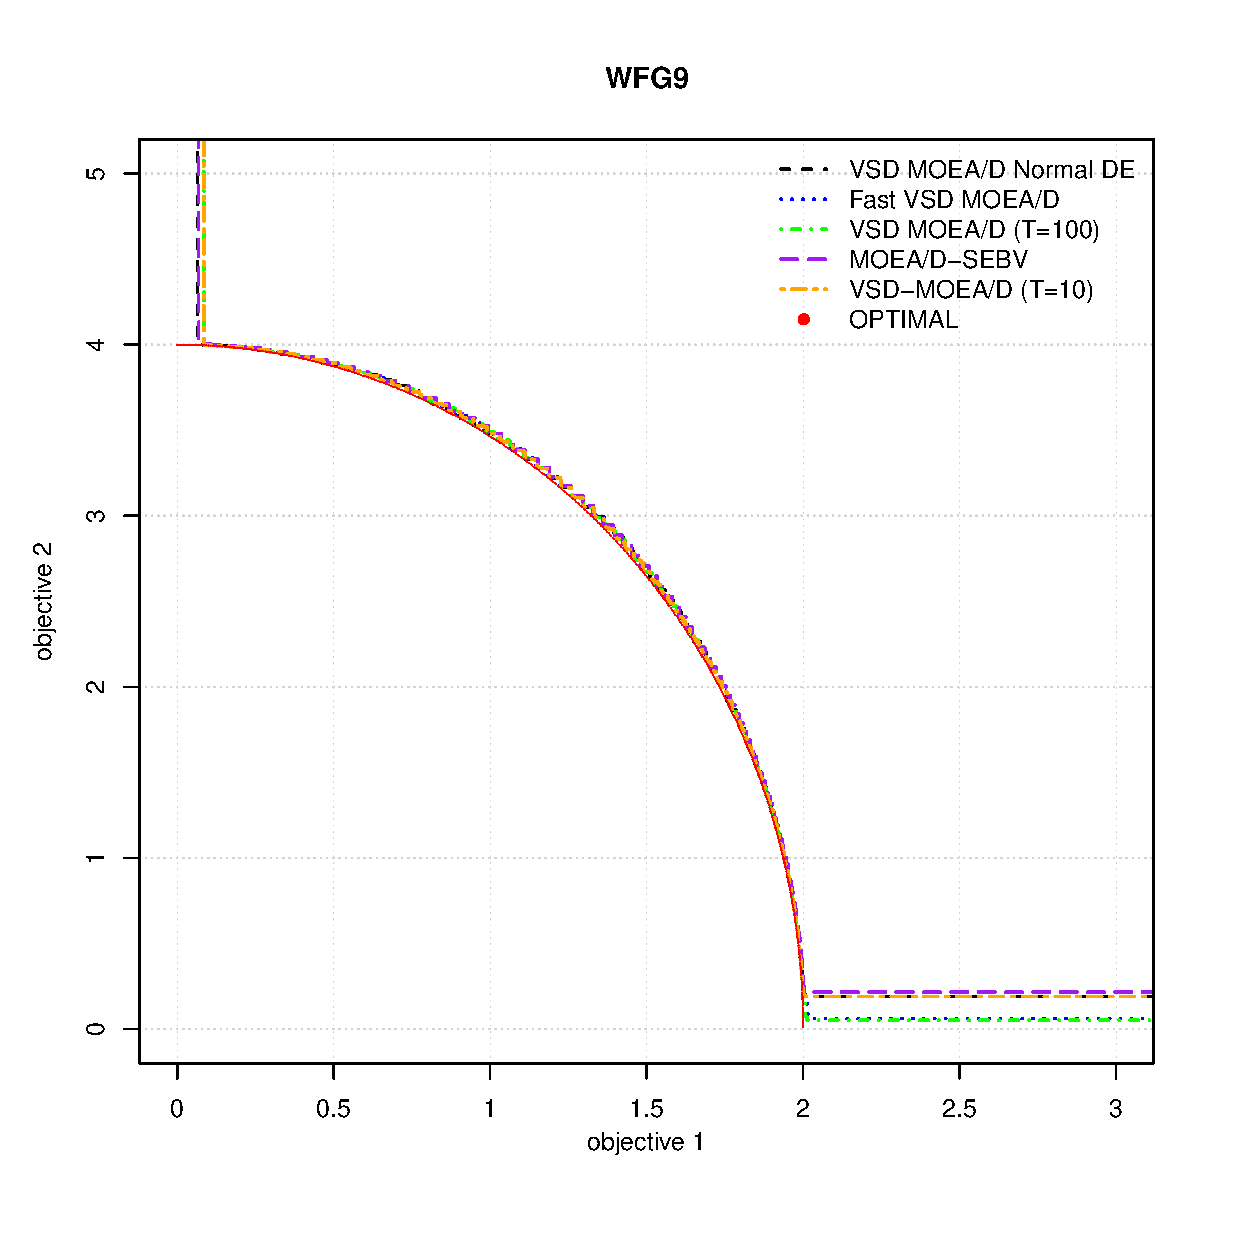
\includegraphics[width=0.40\textwidth]{Surfaces/WFG9.eps}}
% \end{tabular}
% \caption{Analysis of the diversity}
%  \label{fig:Diversity}
% \end{figure*}


%

% \begin{figure*}%[H]
% \centering
% \caption{Attainment Surfaces WFG instances}
% \label{fig:Attainment_Surfaces_State_Art}
% \begin{tabular}{cc}
%    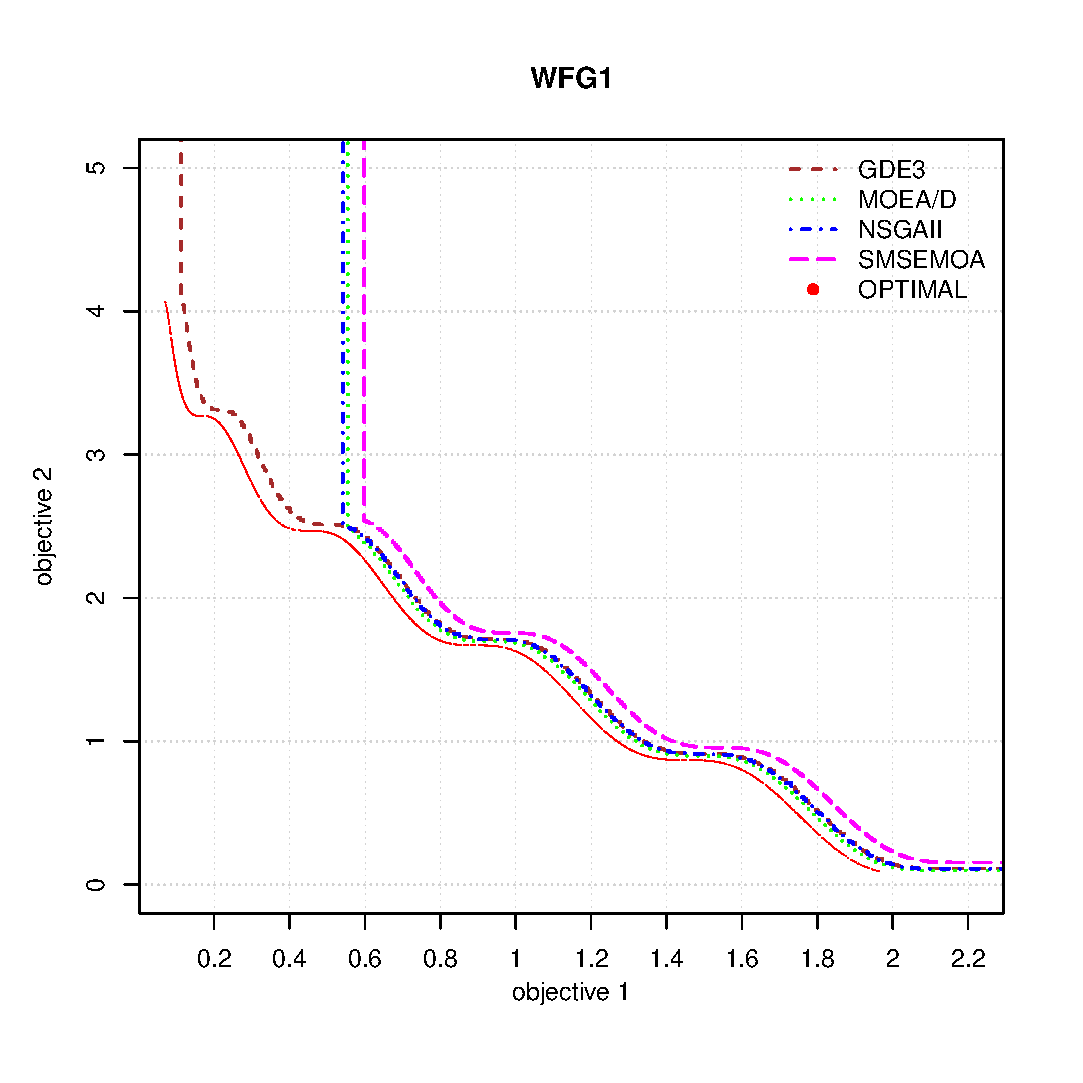
\includegraphics[width=0.4\textwidth]{Surfaces/WFG1.eps} &
%    %\includegraphics[width=0.4\textwidth]{Surfaces/WFG2.eps}  \\
%    %\includegraphics[width=0.3\textwidth]{Surfaces/WFG3.eps} &
%    %\includegraphics[width=0.3\textwidth]{Surfaces/WFG4.eps}  \\
%    \includegraphics[width=0.4\textwidth]{Surfaces/WFG5.eps} 
%    \includegraphics[width=0.4\textwidth]{Surfaces/WFG6.eps}  \\
%    %\includegraphics[width=0.3\textwidth]{Surfaces/WFG7.eps} &
%    \includegraphics[width=0.4\textwidth]{Surfaces/WFG8.eps}&  
%    \includegraphics[width=0.4\textwidth]{Surfaces/WFG9.eps}  
% \multicolumn{2}{c}{\includegraphics[width=0.4\textwidth]{Surfaces/WFG9.eps}}
% \end{tabular}
% \end{figure*}


%



% Please add the following required packages to your document preamble:
% \usepackage{graphicx}
%\begin{table}[]
%\centering
%\scriptsize
%\caption{Pruebas estadísticas HV}
%\label{table:Statistica_Test_Int}
%\resizebox{\textwidth}{!}{%
%\begin{tabular}{c|c|c|c|c|c|c|c|c|c|c|c|c|c|c|c|c|c|c|}
%\cline{2-19}
% & \multicolumn{9}{c|}{NRD-SBX} & \multicolumn{9}{c|}{SBX} \\ \cline{2-19} 
% & \multicolumn{3}{c|}{MOEA/D} & \multicolumn{3}{c|}{NSGA-II} & \multicolumn{3}{c|}{SMS-EMOA} & \multicolumn{3}{c|}{MOEA/D} & \multicolumn{3}{c|}{NSGA-II} & \multicolumn{3}{c|}{SMS-EMOA} \\ \hline
%\multicolumn{1}{|c|}{} & $\uparrow$ & $\downarrow$ & $\longleftrightarrow$ & $\uparrow$ & $\downarrow$ & $\longleftrightarrow$ & $\uparrow$ & $\downarrow$ & $\longleftrightarrow $ & $\uparrow$ & $\downarrow$ & $\longleftrightarrow$ & $\uparrow$ & $\downarrow$ & $\longleftrightarrow$ & $\uparrow$ & $\downarrow$ & $\longleftrightarrow$ \\ \hline
%\multicolumn{1}{|c|}{WFG1} & 3 & 1 & 1 & 5 & 0 & 0 & 2 & 2 & 1 & 1 & 4 & 0 & 2 & 1 & 2 & 0 & 5 & 0 \\ \hline
%\multicolumn{1}{|c|}{WFG2} & 3 & 0 & 2 & 2 & 0 & 3 & 3 & 2 & 0 & 0 & 3 & 2 & 0 & 2 & 3 & 2 & 3 & 0 \\ \hline
%\multicolumn{1}{|c|}{WFG3} & 2 & 2 & 1 & 0 & 5 & 0 & 5 & 0 & 0 & 2 & 2 & 1 & 1 & 4 & 0 & 4 & 1 & 0 \\ \hline
%\multicolumn{1}{|c|}{WFG4} & 2 & 2 & 1 & 0 & 5 & 0 & 4 & 0 & 1 & 2 & 2 & 1 & 1 & 4 & 0 & 4 & 0 & 1 \\ \hline
%\multicolumn{1}{|c|}{WFG5} & 0 & 5 & 0 & 2 & 2 & 1 & 2 & 1 & 2 & 1 & 4 & 0 & 3 & 1 & 1 & 5 & 0 & 0 \\ \hline
%\multicolumn{1}{|c|}{WFG6} & 3 & 0 & 2 & 3 & 1 & 1 & 4 & 0 & 1 & 0 & 3 & 2 & 0 & 3 & 2 & 0 & 3 & 2 \\ \hline
%\multicolumn{1}{|c|}{WFG7} & 2 & 2 & 1 & 0 & 5 & 0 & 4 & 0 & 1 & 2 & 2 & 1 & 1 & 4 & 0 & 4 & 0 & 1 \\ \hline
%\multicolumn{1}{|c|}{WFG8} & 5 & 0 & 0 & 3 & 1 & 1 & 3 & 1 & 1 & 1 & 4 & 0 & 0 & 5 & 0 & 2 & 3 & 0 \\ \hline
%\multicolumn{1}{|c|}{WFG9} & 3 & 1 & 1 & 3 & 1 & 1 & 5 & 0 & 0 & 1 & 3 & 1 & 0 & 5 & 0 & 1 & 3 & 1 \\ \hline
%\multicolumn{1}{|c|}{Total} & \textbf{23} & 13 & 9 & \textbf{18} & 20 & 7 & \textbf{32} & 6 & 7 & \textbf{10} & 27 & 8 & \textbf{8} & 29 & 8 & \textbf{22} & 18 & 5 \\ \hline
%\end{tabular}%
%}
%\end{table}

\begin{table}[t]
\centering
\scriptsize
\caption{Puntuación obtenida por los diferentes algoritmos en base a las pruebas estadísticas}
\label{Tab:HV-score}
\begin{tabular}{c|c|c|c|c|c|c|c|c|c|ccccccccc}
\cline{2-19}
                            & \multicolumn{9}{c|}{NRD-SBX}                                                                                    & \multicolumn{9}{c}{SBX}                                                                                                                                                                                                                                                                                      \\ \hline
\multicolumn{1}{|c|}{}      & \multicolumn{3}{c|}{MOEA/D}         & \multicolumn{3}{c|}{NSGA-II}        & \multicolumn{3}{c|}{SMS-EMOA}       & \multicolumn{3}{c|}{MOEA/D}                                                                        & \multicolumn{3}{c|}{NSGA-II}                                                                       & \multicolumn{3}{c|}{SMS-EMOA}                                                                      \\ \hline
\multicolumn{1}{|c|}{}      & $\uparrow$   & $\downarrow$ & Punt & $\uparrow$   & $\downarrow$ & Punt & $\uparrow$   & $\downarrow$ & Punt & \multicolumn{1}{c|}{$\uparrow$}   & \multicolumn{1}{c|}{$\downarrow$} & \multicolumn{1}{c|}{Punt} & \multicolumn{1}{c|}{$\uparrow$}   & \multicolumn{1}{c|}{$\downarrow$} & \multicolumn{1}{c|}{Punt} & \multicolumn{1}{c|}{$\uparrow$}   & \multicolumn{1}{c|}{$\downarrow$} & \multicolumn{1}{c|}{Punt} \\ \hline
\multicolumn{1}{|c|}{WFG1}  & 2.2          & 0.3          & 1.9   & 3.6          & 0.0          & 3.6   & 1.5          & 0.7          & 0.8   & \multicolumn{1}{c|}{0.7}          & \multicolumn{1}{c|}{2.5}          & \multicolumn{1}{c|}{-1.8}  & \multicolumn{1}{c|}{1.9}          & \multicolumn{1}{c|}{0.3}          & \multicolumn{1}{c|}{1.5}   & \multicolumn{1}{c|}{0.0}          & \multicolumn{1}{c|}{6.0}          & \multicolumn{1}{c|}{-6.0}  \\ \hline
\multicolumn{1}{|c|}{WFG2}  & 0.2          & 0.0          & 0.2   & 0.1          & 0.0          & 0.1   & 0.3          & 0.0          & 0.2   & \multicolumn{1}{c|}{0.0}          & \multicolumn{1}{c|}{0.4}          & \multicolumn{1}{c|}{-0.4}  & \multicolumn{1}{c|}{0.0}          & \multicolumn{1}{c|}{0.1}          & \multicolumn{1}{c|}{-0.1}  & \multicolumn{1}{c|}{0.1}          & \multicolumn{1}{c|}{0.1}          & \multicolumn{1}{c|}{0.0}   \\ \hline
\multicolumn{1}{|c|}{WFG3}  & 0.1          & 0.0          & 0.0   & 0.0          & 0.2          & -0.2  & 0.1          & 0.0          & 0.1   & \multicolumn{1}{c|}{0.1}          & \multicolumn{1}{c|}{0.0}          & \multicolumn{1}{c|}{0.0}   & \multicolumn{1}{c|}{0.0}          & \multicolumn{1}{c|}{0.1}          & \multicolumn{1}{c|}{-0.1}  & \multicolumn{1}{c|}{0.1}          & \multicolumn{1}{c|}{0.0}          & \multicolumn{1}{c|}{0.1}   \\ \hline
\multicolumn{1}{|c|}{WFG4}  & 0.0          & 0.0          & 0.0   & 0.0          & 0.1          & -0.1  & 0.1          & 0.0          & 0.1   & \multicolumn{1}{c|}{0.0}          & \multicolumn{1}{c|}{0.0}          & \multicolumn{1}{c|}{0.0}   & \multicolumn{1}{c|}{0.0}          & \multicolumn{1}{c|}{0.1}          & \multicolumn{1}{c|}{-0.1}  & \multicolumn{1}{c|}{0.1}          & \multicolumn{1}{c|}{0.0}          & \multicolumn{1}{c|}{0.1}   \\ \hline
\multicolumn{1}{|c|}{WFG5}  & 0.0          & 0.5          & -0.5  & 0.2          & 0.0          & 0.2   & 0.2          & 0.0          & 0.2   & \multicolumn{1}{c|}{0.0}          & \multicolumn{1}{c|}{0.4}          & \multicolumn{1}{c|}{-0.3}  & \multicolumn{1}{c|}{0.2}          & \multicolumn{1}{c|}{0.0}          & \multicolumn{1}{c|}{0.2}   & \multicolumn{1}{c|}{0.3}          & \multicolumn{1}{c|}{0.0}          & \multicolumn{1}{c|}{0.3}   \\ \hline
\multicolumn{1}{|c|}{WFG6}  & 0.5          & 0.0          & 0.5   & 0.4          & 0.0          & 0.4   & 0.5          & 0.0          & 0.5   & \multicolumn{1}{c|}{0.0}          & \multicolumn{1}{c|}{0.5}          & \multicolumn{1}{c|}{-0.5}  & \multicolumn{1}{c|}{0.0}          & \multicolumn{1}{c|}{0.5}          & \multicolumn{1}{c|}{-0.5}  & \multicolumn{1}{c|}{0.0}          & \multicolumn{1}{c|}{0.4}          & \multicolumn{1}{c|}{-0.4}  \\ \hline
\multicolumn{1}{|c|}{WFG7}  & 0.0          & 0.0          & 0.0   & 0.0          & 0.1          & -0.1  & 0.1          & 0.0          & 0.1   & \multicolumn{1}{c|}{0.0}          & \multicolumn{1}{c|}{0.0}          & \multicolumn{1}{c|}{0.0}   & \multicolumn{1}{c|}{0.0}          & \multicolumn{1}{c|}{0.1}          & \multicolumn{1}{c|}{-0.1}  & \multicolumn{1}{c|}{0.1}          & \multicolumn{1}{c|}{0.0}          & \multicolumn{1}{c|}{0.1}   \\ \hline
\multicolumn{1}{|c|}{WFG8}  & 2.9          & 0.0          & 2.9   & 1.3          & 0.3          & 1.0   & 0.9          & 0.4          & 0.5   & \multicolumn{1}{c|}{0.1}          & \multicolumn{1}{c|}{1.4}          & \multicolumn{1}{c|}{-1.4}  & \multicolumn{1}{c|}{0.0}          & \multicolumn{1}{c|}{1.7}          & \multicolumn{1}{c|}{-1.7}  & \multicolumn{1}{c|}{0.1}          & \multicolumn{1}{c|}{1.4}          & \multicolumn{1}{c|}{-1.3}  \\ \hline
\multicolumn{1}{|c|}{WFG9}  & 1.0          & 0.1          & 0.9   & 1.0          & 0.0          & 1.0   & 1.3          & 0.0          & 1.3   & \multicolumn{1}{c|}{0.4}          & \multicolumn{1}{c|}{0.7}          & \multicolumn{1}{c|}{-0.4}  & \multicolumn{1}{c|}{0.0}          & \multicolumn{1}{c|}{2.5}          & \multicolumn{1}{c|}{-2.5}  & \multicolumn{1}{c|}{0.4}          & \multicolumn{1}{c|}{0.7}          & \multicolumn{1}{c|}{-0.4}  \\ \hline
\multicolumn{1}{|c|}{Total} & \textbf{6.8} & 0.9          & 6.0   & \textbf{6.6} & 0.8          & 5.9   & \textbf{4.9} & 1.2          & 3.8   & \multicolumn{1}{c|}{\textbf{1.2}} & \multicolumn{1}{c|}{6.1}          & \multicolumn{1}{c|}{-4.8}  & \multicolumn{1}{c|}{\textbf{2.1}} & \multicolumn{1}{c|}{5.3}          & \multicolumn{1}{c|}{-3.2}  & \multicolumn{1}{c|}{\textbf{1.1}} & \multicolumn{1}{c|}{8.7}          & \multicolumn{1}{c|}{-7.6}  \\ \hline
\end{tabular}
\end{table}

% Define some commands to keep the formatting separated from the content 
%\newcommand{\keyword}[1]{\textbf{#1}}
%\newcommand{\tabhead}[1]{\textbf{#1}}
%\newcommand{\code}[1]{\texttt{#1}}
%\newcommand{\file}[1]{\texttt{\bfseries#1}}
%\newcommand{\option}[1]{\texttt{\itshape#1}}

%----------------------------------------------------------------------------------------
